\documentclass[a4paper,11pt]{report}

\usepackage{courier}
% makes listings look much nicer, and also 
% makes keywords in listings boldface (as they should be)

\usepackage{user-guide} % custom style

\makeatletter
\@ifpackageloaded{tex4ht}{%
	% packages/options only used for generating html
	\usepackage{graphicx}	
	
}{%
	% packages/options only used for generating pdf
	\usepackage[pdftex]{graphicx}

	% NextFile is defined by tex4ht, replace it with a NOOP if not generating html
	\newcommand{\NextFile}[1]{}

}
\makeatother

\usepackage[normalem]{ulem}

%%%%%%%%%%%%%%%%%%%%%%%%%%%%%%%%%%%%%%%%%%%%
%%%%%%%%%%%%%%%%%%%%%%%%%%%%%%%%%%%%%%%%%%%%
\usepackage[dvipsnames,svgnames]{xcolor}

\usepackage{soul}

%%%%%%%%%%%%%%%%%%%%%%%%%%%%%%%%%%%%%%%%%%%%
%%%%%%%%%%%%%%%%%%%%%%%%%%%%%%%%%%%%%%%%%%%%

\usepackage[utf8]{inputenc}

\usepackage{tabularx}

%%%%%%%%%%%%%%%%%%%%%%%%%%%%%%%%%%%%%%%%%%%%
%%%%%%%%%%%%%%%%%%%%%%%%%%%%%%%%%%%%%%%%%%%%
\usepackage{listings}

\lstset{language=java,basicstyle=\ttfamily\footnotesize,lineskip=-1pt,keywordstyle=\bfseries\color{blue},commentstyle=\bfseries\color{red},stringstyle=\bfseries\color{ForestGreen},morekeywords={Link,Node,Vehicle},showstringspaces=false,frame=none}
\lstset{language=XML,basicstyle=\ttfamily\footnotesize,tabsize=3,lineskip=-1pt,keywordstyle=\bfseries\color{blue},commentstyle=\bfseries\color{red},stringstyle=\bfseries\color{ForestGreen},showstringspaces=false,frame=none}
% these are my own colors but I am not militant about them.
% I am also not militant about the morekeywords.
% I am, however, somewhat militant about ttfamily font. 
% kai, jul'13


% looks like a bug that listings cannot be defined to be floating except by defining a new environment
% work-around from http://tex.stackexchange.com/questions/43509/lstlisting-ignores-float-setting
\lstnewenvironment{xml-file}[1][]
  {\lstset{language=XML,float=thb,frame=tb,#1}}% \begin{xml-file}[...]
  {} % \end{javalisting}



%%%%%%%%%%%%%%%%%%%%%%%%%%%%%%%%%%%%%%%%%%%%
%%%%%%%%%%%%%%%%%%%%%%%%%%%%%%%%%%%%%%%%%%%%
%% \usepackage{a4wide}
\usepackage{geometry}
\geometry{a4paper,headsep=4mm,top=15mm,bottom=2cm,left=2.0cm,right=3.0cm}

\parindent0pt
\parskip0.3\baselineskip
%%%%%%%%%%%%%%%%%%%%%%%%%%%%%%%%%%%%%%%%%%%%
%%%%%%%%%%%%%%%%%%%%%%%%%%%%%%%%%%%%%%%%%%%%
\usepackage{fancyhdr}
% needs to be after geometry!
 
\lhead{\let\uppercase=\relax\sf\footnotesize\leftmark}
\chead{}
\rhead{\let\uppercase=\relax\sf\footnotesize\rightmark}

\pagestyle{fancy}

\renewcommand{\chaptermark}[1]{%
%
\markboth{\thechapter.\ #1\\}{}
%
}

\renewcommand{\sectionmark}[1]{%
%
\markright{\thesection.\ #1}
%
}
%%%%%%%%%%%%%%%%%%%%%%%%%%%%%%%%%%%%%%%%%%%%
%%%%%%%%%%%%%%%%%%%%%%%%%%%%%%%%%%%%%%%%%%%%
\newcommand{\myemph}[1]{\textcolor{red}{\emph{#1}}}

\newcommand{\todo}[1]{\hl{\emph{TODO #1}}}

\newcommand{\kai}[1]{\textcolor{blue}{[[#1 kai]]}}

\newcommand{\authorsOfDoc}[1]{\vspace{-.5em}\centerline{\hfill Author(s) of this document: #1}\medskip}
\newcommand{\authorsOfCode}[1]{\vspace{-.5em}\centerline{\hfill Main author(s) of the code: #1}\medskip}
\newcommand{\maintainers}[1]{\vspace{-.5em}\centerline{\hfill Maintainer(s): #1}\medskip}

%%%%%%%%%%%%%%%%%%%%%%%%%%%%%%%%%%%%%%%%%%%%
%%%%%%%%%%%%%%%%%%%%%%%%%%%%%%%%%%%%%%%%%%%%
\usepackage{hyperref}
% hyperref needs to be late in calling sequence!


\def\umbruch{\vfill\eject}
\def\umbruch{\relax}

\def\configOptionsNote#1{%
%
\begin{note}
Look into the file {\tt output\_config.xml.gz} in the section {\tt #1} for configuration options.
\end{note}
%
}

%%%%%%%%%%%%%%%%%%%%%%%%%%%%%%%%%%%%%%%%%%%%
%%%%%%%%%%%%%%%%%%%%%%%%%%%%%%%%%%%%%%%%%%%%
%%%%%%%%%%%%%%%%%%%%%%%%%%%%%%%%%%%%%%%%%%%%
%%%%%%%%%%%%%%%%%%%%%%%%%%%%%%%%%%%%%%%%%%%%

\begin{document}
\NextFile{index.html}
\tolerance10000

\title{MATSim User Guide}

\author{%
Marcel~Rieser, % first
%
% everybody in between alphabetic???
Christoph~Dobler,
Thibaut~Dubernet,
Dominik~Grether,
Andreas~Horni, 
Gregor~Lämmel,
Rashid~Waraich,
Michael~Zilske,
%
Kay~W.~Axhausen, % second-last
Kai~Nagel % last
}

\begin{titlepage}
\makeatletter
%\pdfbookmark[1]{Title}{bookmark:Title}
\pagestyle{empty}

\definecolor{Dark}{gray}{.2} 
\definecolor{Medium}{gray}{.55} 
\definecolor{Light}{gray}{.8} 

\makebox(0,0){} % for some strange reason needed, otherwise vfill has no effect
\vspace{3cm}
\par
\raggedright
{\textcolor{Medium}{\fontsize{45}{60}\sffamily\bfseries \@title}}\par
\vspace{1cm}
{\textcolor{Medium}{\titleFontSmall Release Fall 2014 (Version 0.6.0)}}\par
% {\textcolor{Medium}{\titleFontSmall Development Version\\last updated \@date}}\par
\vspace{15cm}
{\titleFontSmall \mdseries\par\@author}\\
\vspace{2cm}
\raggedleft

\includegraphics[width=.33\textwidth]{figures/MATSimLogo_blue.png}

\makeatother
\end{titlepage}
% \maketitle

\umbruch

\section*{Note}

The material found in this document was originally maintained as a collection of web pages.  Those were eventually automatically converted to latex, and incrementally cleaned up since then.  

As a result, leftovers from those web pages can still be found in the document, including lots of links to web pages which could be replaced by internal links in the document, and links to web pages where the material should be inlined into the document.
\\
\hrule

Originally generated 2013-06-12T12:13:34+02:00
\\from matsim.org/docs/userguide
\\but changed since then.



\umbruch

\tableofcontents


%%%%%%%%%%%%%%%%%%%%%%%%%%%%%%%%%%%%%%%%%%%%
%%%%%%%%%%%%%%%%%%%%%%%%%%%%%%%%%%%%%%%%%%%%
\NextFile{Introduction.html}
\chapter{Introduction}

The "tutorial" section contains "reduced" information about how to find your way into matsim.

This "user's guide" section contains additional information,  concentrating on features and details that are not explained in the  tutorials. Clearly, there may be overlap.

\chapter{Features}

The following list shows the key features of MATSim:

\textbf{Fast Dynamic and Agent-Based Traffic Simulation}
\\  In many cases, MATSim only takes a couple of minutes for a single  simulation of a complete day of traffic. This includes the completely  time-dynamic simulation of motorized individual traffic as well as the  handling of agents using other modes of transport.

\textbf{Supports Large Scenarios}
\\  MATSim is able to simulate scenarios with several millions agents or  network with hundreds of thousands of streeets. All you need is a  current, fast desktop computer with plenty of memory. Additionally,  MATSim allows you to only simulate a certain percentage of the traffic,  speeding up the simulation even more while reducing memory consumption,  and still generate useful results.

\textbf{Sophisticated Interactive Visualizer}
\\  Forget aggregated results! MATSim provides a fast Visualizer that can  display the location of each agent in the simulation and what it is  currently doing. It can even connect to a running simulation, allowing  interactively querying agents' states, visualizing agents' routes or  perform live analyses of the network state.

\textbf{Versatile Analyses and Simulation Output}
\\  During the simulation, MATSim collects several key values from the  simulation and outputs them to give you a quick overview of the current  state of the simulation. Among other results, it can compare the  simulated traffic to real world data from counting stations, displaying  the results interactively in Google Earth. Additionally, MATSim provides  detailed output from the traffic microsimulation, which can easily be  parsed by other applications to create your own special analyses.

\textbf{Modular Approach
\\}MATSim  allows for easy replacement or addition of functionality. This allows  you to add your own algorithms for agent-behavior and plug them into  MATSim, or use your own transport simulation while using MATSim's  replanning features.

\textbf{Open Source}
\\ MATSim is  distributed under the Gnu Public License (GPL), which means that MATSim  can be downloaded and used free of charge. Additionally, you get the  complete Source Code which you may modify within certain constraints  (see the license for more details). Written in Java, MATSim runs on all  major operating systems, including Linux, Windows and Mac OS X.

\textbf{Active Development and Versatile Usage of MATSim}
\\  Researchers from several locations are currently working on MATSim.  Core development takes place at the Berlin Institute of Technology (TU  Berlin), the Swiss Federal Institute of Technology (ETH) in Zurich, as  well as in a start-up founded by two former PhD students. Additional  development (as far as we are aware of) currently takes place in South  Africa, Germany (Munich, Karlsruhe) as well as other places around the  world. This distribution of development ensures that MATSim not only  works for one scenario/context, but can be adapted to many different  scenarios.

\NextFile{Overview.html}
\chapter{Overview}
\label{sec:Overview}

\authorsOfDoc{Marcel Rieser}
 
\bigskip

\begin{chapter-intro}
This chapter gives an overview of the major components of MATSim and how they
work together, essentially building the foundation for the MATSim framework.
\end{chapter-intro}

\section{The Major Stages of a MATSim Simulation}

In a typical MATSim simulation, travel demand data is simulated and optimized on
a given transportation network (e.g. a road network, or a multimodal network in
the case when public transport is also considered in the simulation).
The optimization of the demand data is one of the key features of MATSim, making
it suitable to be used for policy studies. In this whole simulation and
optimization process, 5 major stages can be identified:
\begin{itemize}\styleItemize
	\item initial demand
	\item execution
	\item scoring
	\item replanning
	\item analysis
\end{itemize}

These 5 stages are executed in the order shown in
Fig.~\ref{fig:overview:controllerFlow}.
In the following, the responsibilities of each stage is shortly described. The
details for the stages, including what options are available to influence the
stages and how they work, are explained in separate chapters later on.


\begin{figure}[htp]
\begin{center}
  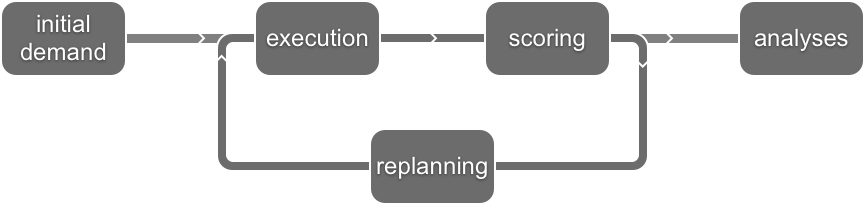
\includegraphics[width=.8\textwidth]{figures/overview/controllerFlow.png}
  \caption{Stages of a MATSim Simulation}
  \label{fig:overview:controllerFlow}
\end{center}
\end{figure}

\paragraph{Initial demand:}
The initial demand describes the mobility behaviour to be simulated. It contains
the full list of agents, and for each agent at least one day plan. A day plan
contains a list of activities (e.g. being \emph{home}, being at \emph{work}) and
trips (e.g. going \emph{by car} to shopping) along with temporal information
(e.g. leaving home \emph{at 7:23 am}, working \emph{until 5:39 pm}) and
additional information (e.g. detailed route going from home to work). Plans
describe the intentions of agents. If agents calculate too optimistically, get
stuck in a traffic jam or miss a bus, it might be that their plan cannot be
realized in the simulation as the agents intended to.

\paragraph{Execution:}
Often also called the \emph{mobility simulation} (or just \emph{mobsim}), the
agents' plans get executed along each other in a representation of the physical
world. This means that the agents and their vehicles are moved around in the
network (the \emph{infrastructure} in the real world). During this execution of
the plans, agents can influence each other by taking up space in the virtual
world. If too many agents want to travel on the same road at a specific time,
they generate a traffic jam in the mobility simulation. This is why the agents'
plans only describe their intentions for a day, but do not actually describe
their day.

\paragraph{Scoring:}
Once the execution of the plans finished, the agents' plans are evaluated based
on their experienced execution. The exact scoring function is customizable, but
generally time spent at activities increases the score, while time spent
travelling decreases it. Agents stuck in a traffic jam thus loose points, while
agents with short and quick trips are able to accumulate more score points by
performing activities for a longer time period.

\paragraph{Replanning:}
As mentioned in the execution stage, agents can be influenced by others and, for
example, get stuck in a traffic jam. During the replanning stage, agents may
modify their plans (actually, they modify copies of the plans, see
Sec.~\ref{sec:Overview:Optimization}) in order to try to avoid situations in the
mobility simulation that lead to bad scores. Typical examples of such
modifications are the modification of activity end times, effectively changing
the start time of the following trip, changing the mode of transport for a trip,
or changing the route for a trip (departure time choice, mode choice, route
choice). In MATSim, these modifications are performed by so-called
\emph{Strategy Modules}.

\paragraph{Analysis:}
At the end of a complete simulation, one is often interested in some key
performance values of the simulation. Examples could be mode shares, miles
travelled in total by all agents, or average trip duration and distance per
mode and hour. Such analyses could either be automatically be performed at then
end, or in a separate post-processing step.

\bigskip

The three stages Execution, Scoring and Replanning are performed iteratively in
order to give the agents multiple opportunities to adapt their plans to the
plans and behaviour of the other agents. This is why MATSim typically performs
multiple \emph{iterations} within one simulation run, consisting of multiple
mobility simulation, scoring and replanning executions, until the end result is
available.

MATSim provides a \emph{Controller} (sadly misspelled as \emph{Controler} in
some places) which implements the iteration loop as shown in
Fig.~\ref{fig:overview:controllerFlow}. This Controller is typically the entry
point for running MATSim simulations, as it handles all aspects from loading all
the required data, configuring the whole setup according to the user's settings,
and iteratively calling the execution, scoring and re-planning stages.
Chpt.~\ref{sec:Running} shows the usage of the Controller in more
detail.


\section{The Optimization Process}
\label{sec:Overview:Optimization}

As outlined above, agents can modify the plans from the initial demand to try to
come up with new variants of the plan that lead to higher scores. The main
concept of the optimization process follows the principles of so-called
\emph{(co-)evolutionary algorithms}. Evolutionary algorithms typically maintain
a set of candidates which are evaluated using a fitness function. New candidates are
generated and evaluated. If they have a bad fitness, they are discarded. If they
have a good fitness, another candidate with a worse fitness is removed from the
set of candidates and the new candidate is added to the set. This is repeated
until no new good candidates are found after some tries.

MATSim implements an evolutionary algorithm for each agent. As all agents are
optimized using their own evolutionary algorithm, the whole system is called a
co-evolutionary algorithm. The set of candidates corresponds to the set of plans
each agent has. New candidates are generated in the replanning stage by making a
copy of an existing plan and modifying the copy. The fitness evaluation is done
by scoring the execution of the plan.
Thus, the replanning stage in MATSim corresponds to the generation of new
candidates of evolutionary algorithms, while the execution and scoring of plans
corresponds to the evaluation of the fitness of the candidates. The repetition 

With each iteration, the goal is that the average score of the executed plans
increase, corresponding to the agents improving their plans such that they can
perform their daily activities as good as possible.
Fig.~\ref{fig:overview:scores} shows how the average score develops in a typical
MATSim simulation over the course of the iterations. Note that the absolute
value of the scores may depend upon the scenario. As can be nicely seen in the
figure, the average executed score typically improves very rapidly in the first
few iterations, but will only improve very slightly in later iterations or even
degrade a few times.


\begin{figure}[htp]
\begin{center}
  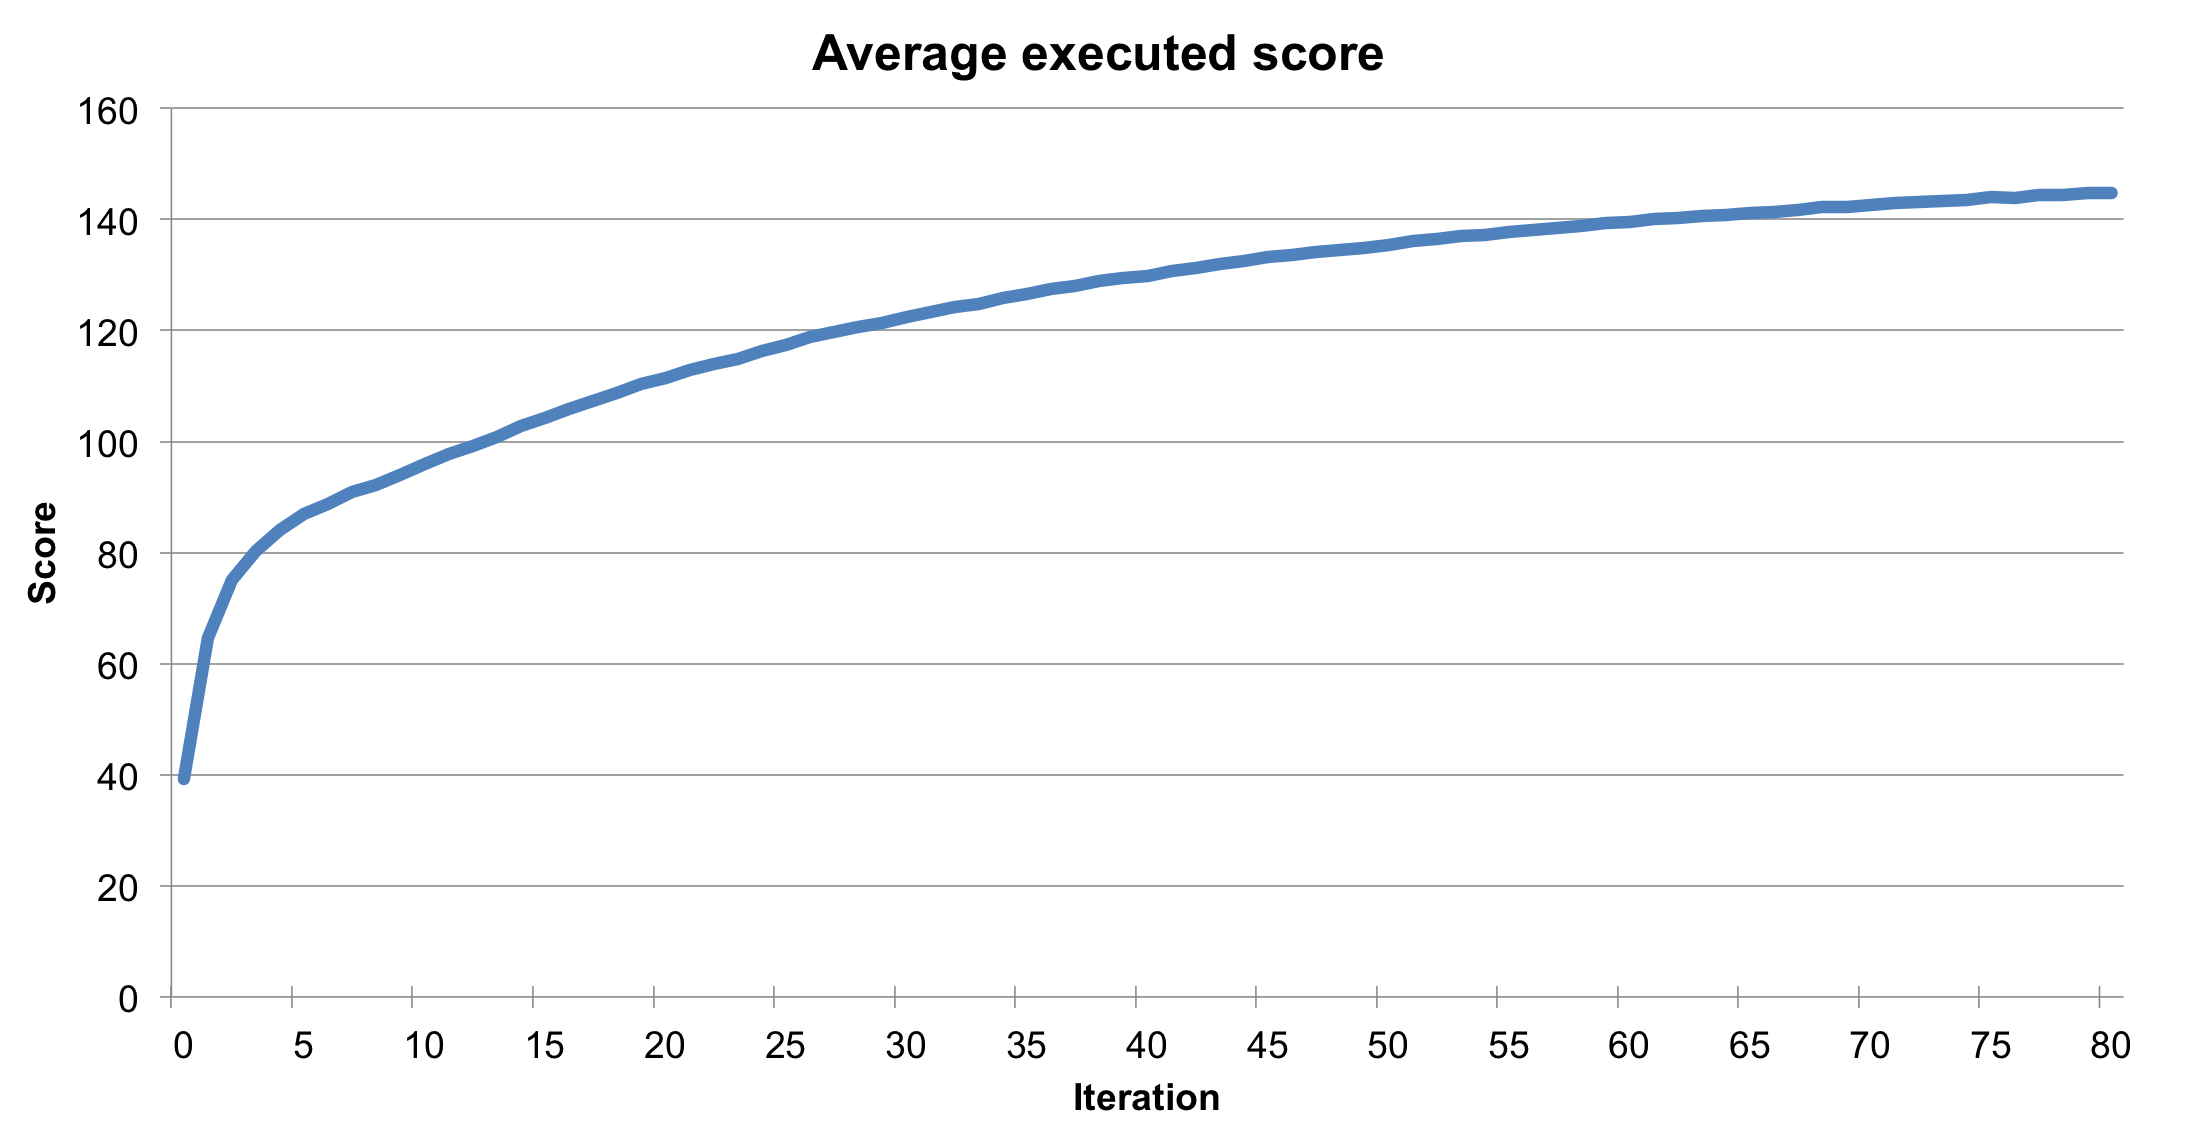
\includegraphics[width=.9\textwidth]{figures/overview/scorestats.png}
  \caption{Tpyical development of the average score of the executed plans over
  the iterations}
  \label{fig:overview:scores}
\end{center}
\end{figure}


\section{Mobility Simulation Events}
The mobility simulation moves the agents around in the virtual world according
to their plans and within the bounds of the ``simulated reality''. The
mobility simulation documents its moves with so-called ``Events''. These events
are small pieces of information describing the action of an object at a
specific time. Examples of such events can be:
\begin{itemize}\styleItemize
  \item An agent finishes an activity
  \item An agent starts a trip
  \item A vehicle enters a road segment
  \item A vehicle leaves a road segment
  \item An agent bordes a public transport vehicle
  \item An agent arrives at a location
  \item An agent starts an activity
\end{itemize}
Each event has a timestamp, a type, and additional attributes required to
describe the action like the agent's id, a link id, an activity type or other
data. In theory, it should be possible to replay the mobility simulation just by
the information stored in the events. While plans describe the agents' plan for
a day, the events describe how the agents' day actually was (according to the
simulation).

As the events are so basic, each agent typically generates hundreds of events
during one execution of a mobility simulation. In total, the number of events
generated by a mobility simulation can easily reach a million or more, with
large simulations even generating more than a billion events. But as the events
really describe all the details from the execution of the plans, it is possible
to extract mostly any kind of aggregated data one is interested in. Practically
all analyses of MATSim simulations make use of events to calculate some data.
Examples of such analyses are the average duration of an activity, average trip
duration or distance, mode shares per time window, number of passengers in
specific transit lines and many more.

The scoring of the executed plans makes use of events to find out how much time
agents spent at activities or for travelling. Some replanning modules might
make use of events as well: The router for example can use the information
contained in events to figure out what links are jammed at certain times and
route agents around that jam when creating new plans.


\section{Customizability}
MATSim is designed to be modular. Nearly all parts can be customized, replaced
or enhanced with custom functionality. Some customizations are easier than
others. Replacing the mobility simulation for additonal behaviour might be one
of the hardest things to achieve. Changing the replanning on the other hand is
quite easy, especially as there is already a number of modules available for
different replanning needs which can be activiated and used without programming
and only by modifying the configuration file. This guide will mostly focus on
functionality available in a standard release of MATSim that can be used just by
making changes to the configuration file, and not on enhancing MATSim by
programming custom functionality.


\begin{note}
In order to work with MATSim, you should know the \emph{5 major stages} of a
MATSim simulation, why MATSim uses \emph{iterations} and understand conceptually what
data is contained in \emph{plans} and what data is contained in \emph{events}.
\end{note}

\authorsOfDoc{Kai Nagel}

\bigskip

In  many cases, MATSim uses a terminology that is different from the  mainstream terminology. In most cases, the reason is that the  concepts are only similar, but not identical, and we wanted to avoid the  confusion of using the same term for aspects that are similar but not  identical. The following attempts some commented approximate  "translations" from more standard teminology to MATSim terminology.

\section{Choice set $\to$ ``plan set'' of an agent}

During MATSim iterations, agent accumulate   plans. This can be  interpreted as building a choice set over  time. A  problem is that the  process that generates the choice  set at this  point is not systematic.

\paragraph{Possible future developments:} Once it has been made explicit that "plans generation" means "choice set generation", the terminology may be made standard.

\section{Choice set generation $\to$ Time mutation/re-route/... ; "innovation"}

As said above, the set of MATSim plans can   be seen as this agent's choice set. MATSim generates new plans   "on-the-fly", i.e. while the simulation is running. We sometimes  call  this "innovation", since agents create new plans (= add entries to  the  choice set), rather than choosing between existing plans.

\section{Choice set generation, choice $\to$ replanning}

In MATSim, there is no strict separation between "choice set  generation" and "choice": at the replanning step, for each agent, a  replanning strategy is randomly choosen. This strategy may consist in  selecting a random plan to use to generate a new plan by mutation  ("choice set generation" part), or just to select a past plan based on  the experienced score ("choice" part).

\section{Convergence $\to$ learning rate}

Scores in matsim are computed as
\[
score_{new} = (1-\alpha) \cdot score_{old} +   \alpha \cdot score_{sim} \ , 
\]
where $score_{sim}$ is the score that is obtained from   the execution of the plans (= network loading).

\section{Mu (logit model scaling factor) $\to$ beta\_brain}


MATSim scoring function: 
\[
{\tt BrainExpBeta} \cdot \sum_i \beta_i \, x_i
\]

Typical logit model formulation: 
\[
\mu \cdot \sum_i \beta_i \, x_i
\]

As is well known, $\mu$ or $\beta_i$ are not independently
identifiable from estimation. For simulation, they are hence somewhat
arbitrary. The default value for "BrainExpBeta" is 2 for historical
reasons, but it should be set to 1 if the parameters of the scoring
function are estimated rather than hand-calibrated.

\paragraph{Possible future development:}

Default value of \verb$BrainExpBeta$ should be set to $1.$ instead of $2.$.


\section{Multinomial logit $\to$ ExpBetaPlanSelector}


\paragraph{Comments:}
\begin{itemize}
	\item The main problem is that one needs to keep in mind how the choice set is constructed (see above).
	\item In most simulations, we use ExpBetaPlanChanger instead, which is a   Metropolis Monte Carlo variant of making multinomial logit draws
\end{itemize}

\paragraph{Possible future developments:} None of this is  ideal,  since, after the introduction of a policy, it is not clear which   behavioral switches are due to the policy, and which are due to   sampling. In theory, one should have unbiased samples before and  after  the introduction of the policy, but at this point this is not   implemented and it is also computationally considerably more expensive   than what is done now.

\section{Network loading $\to$ mobsim, mobility simulation, physical simulation}


The standard terminology has the "network   loading" on the "supply  side". In my (KN's) view, the  "simulation of  the physical system" is  not the supply side, but what  in economics is  called "technology". This  can for example be  seen in the fact that  "lane changing" is part of the  mobsim, but this  is, in my view, not a  "supply side" aspect.

\paragraph{Possible future developments:} May switch to "network loading" if there is agreement that this is a better name.

\section{Stationary $\to$ relaxed}

``stationary'' means that the probability   distribution does not shift any  more. However, as long as  "innovation"  is still switched in on MATSim  (new routes, new times,  ...), the  result is not truly stationary. Thus  we avoid the  word. If innovation  is switched off, the result is indeed a   statinary process, but limited  to the set of plans that every agent has   at that point in time.

\paragraph{Possible future developments:} not clear. Minimally, publications should be precise.

\paragraph{Configuration:}
\begin{lstlisting}{language=XML}
<module name="strategy" >
	<!-- iteration after which module will be disabled.  ... -->
	<param name="ModuleDisableAfterIteration_1" value="null" />
	<param name="ModuleDisableAfterIteration_2" value="950" />

	<!-- probability that a strategy is applied to a given person.  ... -->
	<param name="ModuleProbability_1" value="0.9" />
	<param name="ModuleProbability_2" value="0.1" />

	<!-- name of strategy ... -->
	<param name="Module_1" value="ChangeExpBeta" />
	<param name="Module_2" value="ReRoute" />

	<!-- maximum number of plans per agent ... -->
	<param name="maxAgentPlanMemorySize" value="4" />
</module>
\end{lstlisting}


The above means:
\begin{itemize}
	\item StrategyModule "ReRoute" (= innovative Module, produces plans with new routes) is switched off after iteration 950.
	\item StrategyModule "ChangeExpBeta" (= non-innovative Module, switches between existing plans) is never switched off.
	\item If an agent ever ends up with more than 4 plans, plans are deleted  until she is back to 4 plans. (Deletion goes via a  "PlanSelectorForRemoval", which affects the choice set, and thus more  thought needs to go into this. Currently, the plan with the worst  score is removed.)
\end{itemize}

\section{Utility $\leftrightarrow$ score}


At least when using random utility models (such as multinomial logit   aka ExpBeta...), the score has the same function as the deterministic   utility.

\NextFile{RunningMATSim.html}
\chapter{Running MATSim}
\label{sec:Running}

\authorsOfDoc{Marcel Rieser}
 
\bigskip

\begin{chapter-intro}
MATSim comes without any easy to use graphical interface. Instead, it uses text
files for configuration and uses a command line interface to start simulations.
This chapter shows you how to start MATSim simulations in a number of different
computing environments.
\end{chapter-intro}


\section{Prerequisites}

MATSim is written in Java, a programming language which allows to write
applications that run on a large variety of computers. As scenarios can become
quite large, they may consume large amounts of memory (RAM). Very large
scenarios should be run on dedicated servers with enough resources.

In general, to use MATSim, the following requirements must be met:
\begin{itemize}\styleItemize
  \item Java SE 7 must be installed. The latest version of the Java Runtime
  Environment (JRE) can be downloaded from \url{http://java.oracle.com}.
  \item Have at least 2 GB memory for running the examples. For larger
  scenarios, more memory will be required.
  \item Have enough free hard drive space. The provided examples will occupy
  only a few megabytes, but large scenarios can easily use multiple gigabytes of
  disk space.
  \item Last but not least, you need a version of MATSim.
\end{itemize}
This chapter assumes you are using a release (or nightly build) of MATSim which
comes pre-packaged as a jar-file. This chapter will not explain how to compile
and run MATSim based on its program source files. In the remainder of this
chapter, {\tt matsim.jar} will be used to refer to the jar-file of MATSim. The
actual name might differ, e.g. it might include a version number like {\tt
matsim-0.6.0.jar} or {\tt matsim-20140114.jar}.


\section{Using MATSim from a Command Line}
To run MATSim, one needs a configuration file and an estimation, how much memory
the simulation will consume (Don't fear this, you'll get used to this quite
fast). As MATSim comes without graphical user interface, it needs to be run on
the command line. In Linux or Mac OS X, this is typically done using a Terminal
application. In Windows, the Power Shell or Command Prompt can be used.

On the command line, type the following command, but substitute the correct
paths:
\begin{verbatim}
java -Xmx512m -cp /path/to/matsim.jar
      org.matsim.run.Controler /path/to/config.xml
\end{verbatim}
Note that the commands should always be written on one line, they are shown in
this tutorial on multiple lines only for readability.

As an example, on Linux this could look like:
\begin{verbatim}
java -Xmx512m -cp /home/username/matsim/matsim.jar 
      org.matsim.run.Controler /home/user/matsim/input/config.xml
\end{verbatim}

On Mac OS X, it could look like this:
\begin{verbatim}
java -Xmx512m -cp /Users/username/matsim/matsim.jar 
      org.matsim.run.Controler /Users/user/matsim/input/config.xml
\end{verbatim}

On Windows, an example command could be:
\begin{verbatim}
java -Xmx512m -cp C:\MATSim\matsim.jar 
      org.matsim.run.Controler C:\MATSim\input\config.xml
\end{verbatim}

Such a command exists of multiple parts:
\begin{itemize}
  \item {\tt java} tells the system that you want to run Java.
  \item {\tt -Xmx512m} tells Java that it should use up to 512 MB of memory.
  This is typically enough to run the small examples. For larger scenarios, you
  might need more memory: {\tt -Xmx3g} would allow Java to use up to 3 GB of
  memory.
  \item {\tt -cp /path/to/matsim.jar} tells Java where to find the MATSim code.
  \item {\tt org.matsim.run.Controler} tells Java which class (think of ``entry
  point'') it should start running. In most cases, the default MATSim Controler
  is the class you'll need to run simulations.
  \item {\tt /path/to/config.xml} tells MATSim which config file is to be used.
\end{itemize}

In the case you have relative paths in your config file, make sure to start
MATSim in the correct directory. It will interpret all relative paths based on
the directory where the Java process got started, and not where the config file
is located.


\NextFile{BuildingScenarios.html}
\chapter{Building New Scenarios}
\label{sec:BuildingScenarios}

\authorsOfDoc{Marcel Rieser}
 
\bigskip

\begin{chapter-intro}
Starting a new scenario (our term for the application of MATSim to a 
region/area) can appear quite cumbersome at the first glace, as a lot of data
preparation may be required. This chapter gives first an overview of the input
data typically required for running a MATSim scenario, and then gives examples
how such data is generated for existing scenarios.
\end{chapter-intro}

\section{Typical Input Data Sets}
MATSim uses multiple files to store the different types of data it uses for the
simulation. Tab.~\ref{tab:BuildingScenarios:InputDataSets} gives an
overview over files you may typically encounter when working with MATSim.

Not all files are always required. Very simple simulations can be run
only with a configuration file and the description of the network and
the population containing the agents' plans. For additional functionality, e.g.
for the simulation of public transport, additional files might be required.

\begin{table}[htp]
\begin{tabular}{ll}
\hline
{\tt config.xml}          & configuration options for MATSim \\
{\tt network.xml}         & description of the (road) network \\
{\tt population.xml}      & the travel demand, i.e. the list of agents
and their day plans
\\
{\tt facilities.xml}      & information about locations where
activities can be performed\\
{\tt transitSchedule.xml} & information about transit stop locations
and transit services\\
{\tt transitVehicles.xml} & description of the vehicles used for
public transport services\\
{\tt counts.xml}          & hourly volumes from real-world counting
stations for comparison\\
\hline
\end{tabular}
\caption{Files often used with MATSim}
\label{tab:BuildingScenarios:InputDataSets}
\end{table}

In the following, small examples of these files will be shown and the data they
contain discussed.

\begin{note}
Some of the files, especially {\tt population.xml}, but also {\tt network.xml} 
or {\tt facilities.xml}, might get quite large. To save space, MATSim supports
reading and writing the data in a compressed format. MATSim uses  
GZIP-compression for this. Thus, in many cases, the file names have the 
additional suffix {\tt .gz}, as in {\tt population.xml.gz}. MATSim automatically
detects if files are compressed or should be written compressed based on the 
filename.
\end{note}

\subsection{Configuration}

\begin{xml-file}[caption=An example of a config.xml,
label=lst:BuildingScenarios:configXml]
<?xml version="1.0" ?>
<!DOCTYPE config SYSTEM "http://www.matsim.org/files/dtd/config_v1.dtd">
<config>

	<module name="network">
		<param name="inputNetworkFile" value="example/network.xml" />
	</module>

	<module name="plans">
		<param name="inputPlansFile" value="example/population.xml.gz" />
	</module>

	<module name="controler">
		<param name="outputDirectory" value="./output/" />
		<param name="firstIteration" value="0" />
		<param name="lastIteration" value="10" />
	</module>
	
</config>
\end{xml-file}

The configuration file, often just referred to as \emph{config file}
or as \emph{config.xml}, builds the connection between the user and MATSim.
It contains a list of settings which influence how the simulation behaves.

All configuration parameters are simple pairs of a parameter name and a
parameter value. The parameters are grouped into logical groups. For example,
there is a group with settings related to the Controler like the number of
iterations, or there is another group with settings related to the simulation,
e.g. the end time of the simulation.
Listing~\ref{lst:BuildingScenarios:configXml} shows a very short example of a
configuration file which specifies the network and travel demand data to be used
along with some settings for the Controler.

The list of available parameters and valid parameter values may vary from
release to release. Although we try to keep this stable, due to changes in the
software, most notably by new features, settings may change. To get a list of
all available settings currently available, run the following command:
\begin{lstlisting}
java -cp matsim.jar org.matsim.run.CreateFullConfig fullConfig.xml
\end{lstlisting}
This command will create a new config file {\tt fullConfig.xml} which contains
the full list of available parameters along with their default values. This
makes it easy to see what settings are available. To use and modify certain
settings, the lines with the corresponding parameters can be copied to the
config file specific for the scenario to be simulated and the parameter values
be modified in that file.


\subsection{Network}

\begin{xml-file}[caption=An example of a network.xml,
label=lst:BuildingScenarios:networkXml]
<?xml version="1.0" encoding="utf-8"?>
<!DOCTYPE network SYSTEM "http://www.matsim.org/files/dtd/network_v1.dtd">

<network name="example network">
	<nodes>
		<node id="1" x="0.0" y="0.0"/>
		<node id="2" x="1000.0" y="0.0"/>
		<node id="3" x="1000.0" y="1000.0"/>
	</nodes>
	<links>
		<link id="1" from="1" to="2" length="3000.00" capacity="3600" 
		                           freespeed="27.78" permlanes="2" modes="car" />
		<link id="2" from="2" to="3" length="4000.00" capacity="1800" 
		                           freespeed="27.78" permlanes="1" modes="car" />
		<link id="3" from="3" to="2" length="4000.00" capacity="1800" 
		                           freespeed="27.78" permlanes="1" modes="car" />
		<link id="4" from="3" to="1" length="6000.00" capacity="3600" 
		                           freespeed="27.78" permlanes="2" modes="car" />
	</links>
</network>
\end{xml-file}

The network describes the infrastucture on which the agents (or the vehicles,
respectively), can move around. The network consists of \emph{nodes} and
\emph{links} (in graph theory, these are typically called \emph{vertices} and
\emph{edges}). Listing~\ref{lst:BuildingScenarios:networkXml} shows an example
of a simple description of a network in MATSim's XML data format.

Each element has an identifier \emph{id}. Nodes are described by an X and a Y
coordinate value. Links have more attributes: The \emph{from} and \emph{to}
attribute reference nodes and describe the geometry of the network. Additional
attributes describe the traffic-related aspects of the network:
\begin{itemize}\styleItemize
  \item the \emph{length} of the link, typically in meters (see
  Sec.~\ref{sec:BuildingScenarios:Units}).
  \item the \emph{flow capacity} of the link, i.e. the number of vehicles that
  can pass the link, typically in vehicles per hour.
  \item the \emph{freespeed} is the maximum speed at which vehicles are allowed
  to travel along the link, typically in meters per seconds.
  \item the \emph{number of lanes} ({\tt} permlanes) available in the direction
  specified by the {\tt from} and {\tt to} nodes.
  \item the list of \emph{modes} allowed on the link. This is a comma-separated
  list, e.g. {\tt modes="car,bike,taxi"}.
\end{itemize}
Note that all links are uni-directional. If a road can be travelled in both
directions, two links have to be defined with alternating {\tt to} and {\tt
from} attributes (see links with id {\tt 2} and {\tt 3} in the example given in
Listing~\ref{lst:BuildingScenarios:networkXml}).
Thus, the network can be seen as a directed graph.

\subsection{Demand}

The travel demand for MATSim is described by the agents' day plans. The full set
of agents is typically the \emph{population}, hence the filename {\tt
population.xml}. Alternatively, {\tt plans.xml} is also commonly used in MATSim,
as the population file essentially contains a list of day plans.

The population contains the data in a hierarchical structure, as shown in
Listing~\ref{lst:BuildingScenarios:populationXml}:
\begin{itemize}\styleItemize
  \item The population contains a list of persons.
  \item Each person contains a list of plans.
  \item Each plan contains a list of \emph{Activities} and \emph{Legs}.
\end{itemize}
Exactly one plan per person is marked as \emph{selected}. The selected plan of
each agent is the plan that gets executed by the mobility simulation. During the
replanning stage, a different plan might get marked as being selected. A plan
can contain a score as attribute. The score gets calculated and stored in the
plan during the scoring stage, after the plan was executed by the mobility
simulation.

The list of activities and legs in each plan describe the planned actions by
each agent. Activities have a type assigned and have---except for the last
activity in a day plan---an end time defined (There are some exceptions where
activities have a duration instead of an end time. Such activities are often
automatically generated by routing algorithms and are thus not described in
this guide). To describe the location where an activity takes place, the
activity is either assigned a coordinate by giving an x and y attribute value,
or has a link assigned which describes from which link the activity can be
reached. As the simulation requires the link attribute, the Controler calculates
the nearest link for a given coordinate in the case the attribute is missing and
only an x and y coordinate value is given or any activity.

\begin{xml-file}[caption=An example of a population.xml,
label=lst:BuildingScenarios:populationXml]
<?xml version="1.0" encoding="utf-8"?>
<!DOCTYPE population SYSTEM "http://www.matsim.org/files/dtd/population_v5.dtd">
<population>
	<person id="1">
		<plan selected="yes" score="93.2987721">
			<act type="home" link="1" end_time="07:16:23" />
			<leg mode="car">
				<route type="links">1 2 3</route>
			</leg>
			<act type="work" link="3" end_time="17:38:34" />
			<leg mode="car">
				<route type="links">3 1</route>
			</leg>
			<act type="home" link="1" />
		</plan>
	</person>
	<person id="2">
		<plan selected="yes" score="144.39002">
			\ldots
		</plan>
	</person>
</population>
\end{xml-file}

Legs describe how agents plan to travel from one location to the next one. Each
leg must have a transport mode assigned. Optionally, legs may have an
attribute {\tt trav\_time} which describes the expected travel time for this
leg. For a leg to be simulated, it must contain a route. The format of a
route depends on the mode of a leg. For car-legs, the route lists the links that
the agent has to travel along in the given order, while for transit-legs
information about the stop locations and expected transit services are stored.

An agent starts a leg directly after the previous activity (or leg) has ended.
Depending on the mode, the mobility simulation might handle the agent
differently. By default, car- and transit-legs are well-supported by the
mobility simulation. If the mobsim encounters a mode it does not know, it
defaults to \emph{teleportation}: In this case, the agent is removed from the
simulated reality, and after the leg's expected travel time has passed,
re-inserted at the agent's target location.

\bigskip

The population data format is one of the most central data structures in
MATSim and might be a bit overwhelming at first. Luckily, to get started, only a
small subset must be known of it.
Listing~\ref{lst:BuildingScenarios:minimalPopulationXml} shows how a minimal
population file could look like. Most notably, the following simplications can
be made:
\begin{itemize}\styleItemize
  \item Each person needs exactly one plan.
  \item The plan does not need to be selected or have a score.
  \item Activities can be located just by their coordinates.
  \item Activities should have a somewhat meaningful end-time.
  \item Legs only need a mode, but no routes.
\end{itemize}
When a simulation is started, MATSim's Controler will load such a file and then
automatically assign the nearest linnk to each activity and calculate a suitable
route for each leg. This makes it easy to get started quickly.

\begin{xml-file}[caption=Minimal population.xml required to start MATSim,
label=lst:BuildingScenarios:minimalPopulationXml]
<?xml version="1.0" encoding="utf-8"?>
<!DOCTYPE population SYSTEM "http://www.matsim.org/files/dtd/population_v5.dtd">
<population>
	<person id="1">
		<plan>
			<act type="home" x="5.0" y="8.0" end_time="08:00:00" />
			<leg mode="car">
			</leg>
			<act type="work" x="1500.0" y="890.0" end_time="17:30:00" />
			<leg mode="car">
			</leg>
			<act type="home" x="5.0" y="8.0" />
		</plan>
	</person>
	<person id="2">
		\ldots
	</person>
</population>
\end{xml-file}

\subsection{Public Transport}
\begin{xml-file}[caption=An example of a schedule.xml]
<?xml version="1.0" encoding="UTF-8"?>
<!DOCTYPE transitSchedule SYSTEM "http://www.matsim.org/files/dtd/transitSchedule_v1.dtd">
<transitSchedule>
	<transitStops>
		<stopFacility id="1" x="990.0"  y="0.0"   name="Adorf"    linkRefId="1" isBlocking="false"/>
		<stopFacility id="2" x="1100.0" y="980.0" name="Beweiler" linkRefId="2" isBlocking="true"/>
		<stopFacility id="3" x="0.0"    y="10.0"  name="Cestadt"  linkRefId="3" isBlocking="false"/>
	</transitStops>
	<transitLine id="Blue Line">
		<transitRoute id="1">
			<description>Just a comment.</description>
			<transportMode>bus</transportMode>
			<routeProfile>
				<stop refId="1" departureOffset="00:00:00"/>
				<stop refId="2" arrivalOffset="00:02:30" departureOffset="00:03:00" awaitDeparture="true"/>
				<stop refId="3" arrivalOffset="00:05:00" awaitDeparture="true"/>
			</routeProfile>
			<route>
				<link refId="1"/>
				<link refId="2"/>
				<link refId="3"/>
			</route>
			<departures>
				<departure id="1" departureTime="07:00:00" vehicleRefId="12"/>
				<departure id="2" departureTime="07:05:00" vehicleRefId="23"/>
				<departure id="3" departureTime="07:10:00" vehicleRefId="34"/>
			</departures>
		</transitRoute>
	</transitLine>
</transitSchedule>
\end{xml-file}

\begin{xml-file}[caption=An example of transitVehicles.xml]
<?xml version="1.0" encoding="UTF-8"?>
<vehicleDefinitions xmlns="http://www.matsim.org/files/dtd"
       xmlns:xsi="http://www.w3.org/2001/XMLSchema-instance"
       xsi:schemaLocation="http://www.matsim.org/files/dtd http://www.matsim.org/files/dtd/vehicleDefinitions_v1.0.xsd">
	<vehicleType id="1">
		<description>Small Train</description>
		<capacity>
			<seats persons="50"/>
			<standingRoom persons="30"/>
		</capacity>
		<length meter="50.0"/>
	</vehicleType>
	<vehicle id="tr_1" type="1"/>
	<vehicle id="tr_2" type="1"/>
</vehicleDefinitions>
\end{xml-file}

\todo{MR}


\subsection{Counts}
\begin{xml-file}[caption=An example of a counts.xml]
<?xml version="1.0" encoding="UTF-8"?>
<counts xmlns:xsi="http://www.w3.org/2001/XMLSchema-instance" 
        xsi:noNamespaceSchemaLocation="http://matsim.org/files/dtd/counts_v1.xsd" 
        name="test" desc="test counting stations" year="2014">
	<count loc_id="2" cs_id="005">
		<volume h="1" val="10.0"></volume>
		<volume h="2" val="1.0"></volume>
		<volume h="3" val="2.0"></volume>
		<volume h="4" val="3.0"></volume>
		<volume h="5" val="4.0"></volume>
		<volume h="6" val="5.0"></volume>
		<volume h="7" val="6.0"></volume>
		<volume h="8" val="7.0"></volume>
		<volume h="9" val="8.0"></volume>
		<volume h="10" val="9.0"></volume>
		<volume h="11" val="10.0"></volume>
		<volume h="12" val="11.0"></volume>
		<volume h="13" val="12.0"></volume>
		<volume h="14" val="13.0"></volume>
		<volume h="15" val="14.0"></volume>
		<volume h="16" val="15.0"></volume>
		<volume h="17" val="16.0"></volume>
		<volume h="18" val="17.0"></volume>
		<volume h="19" val="18.0"></volume>
		<volume h="20" val="19.0"></volume>
		<volume h="21" val="20.0"></volume>
		<volume h="22" val="21.0"></volume>
		<volume h="23" val="22.0"></volume>
		<volume h="24" val="23.0"></volume>
	</count>
</counts>
\end{xml-file}

\todo{MR}

\section{Units and Conventions Used}
\label{sec:BuildingScenarios:Units}
\todo{MR: id: any string, but please no white spaces and commas, coordinate system, mostly meter, seconds}

old stuff from here
================

Given these two data items, you can already start building your own
scenario.The "\href{http://www.matsim.org/docs/tutorials/learningIn3days}{Learning MATSim in 3 days}"-Tutorial gives you an introduction on how to build your own scenario.

\subsubsection{Import from VISUM}

See \href{http://matsim.org/javadoc/org/matsim/visum/package-summary.html}{here for javadoc}, and \href{http://matsim.org/xref/org/matsim/visum/package-summary.html}{here for code}.

\subsubsection{Programming}

In many cases, using pre-configured software is not possible because  there are just too many possibilities of how input could look like.  Although matsim is not there yet, these should be api-only use cases,  i.e. they should only use the "stable" api. Therefore, the  following are under the api-users section of the documentation:
\begin{itemize}
	\item Additional information about network generation is \href{http://matsim.org/node/588}{here}.
	\item additional information about initial demand generation is \href{http://matsim.org/node/340}{here}.
\end{itemize}

\subsubsection{Information concerning specific scenarios}

The following sections contains various information for building a scenario that presumably goes beyond what is in the tutorial.

\section{Coordinate Systems in MATSim}

For  some operations, MATSim must know about the coordinate system your data  is in. For example, If you want to generate kml-Output for  Counts-Validation, MATSim has to convert the coordinates in your network  to WGS84, the coordinate system used by Google Earth.


\subsubsection{Specifying the Coordinate System used}

You can specify the coordinate system in the config-file:
\begin{lstlisting}{language=XML}
<module name="global">
  <param name="coordinateSystem" value="CH1903LV1903" />
</module>
\end{lstlisting}

The value specified for the coordinateSystem parameter can be:
\begin{itemize}
	\item The short-name of a coordinate system known to MATSim. We define  names for coordinate systems we use regularly in our work. These names  are currently defined in \href{http://matsim.svn.sourceforge.net/viewvc/matsim/matsim/trunk/src/main/java/org/matsim/core/utils/geometry/transformations/TransformationFactory.java?view=markup}{TransformationFactory}. The short-name 
\texttt{Atlantis}  stands for an artificial coordinate system which maps our examples  without relation to the real world somewhere in to the Atlantic ocean.
	\item Well-Known-Text (\href{http://www.geoapi.org/snapshot/javadoc/org/opengis/referencing/doc-files/WKT.html}{WKT})  description of a coordinate system as they are supported by Geotools.  This variant is not very readable, but allows one to experiment also in  regions where MATSim does not provide a short-name for. Examples of WKT  can be found in the MATSim-class \href{http://matsim.svn.sourceforge.net/viewvc/matsim/matsim/trunk/src/main/java/org/matsim/core/utils/geometry/geotools/MGC.java?view=markup}{MGC}(in the 
\texttt{transformations} map).
\end{itemize}

\subsubsection{Notes about Coordinate Systems}

As the distance calculation in WGS84-coordinates (or any spherical coordinates) is rather complex (a simple \href{http://en.wikipedia.org/wiki/Pythagorean_theorem}{Pythagoras} is not enough), we advise people to use a \href{http://en.wikipedia.org/wiki/Coordinate_system}{Cartesian coordinate systems},  preferable where one unit corresponds to one meter. Using such a  coordinate system is a pre-requisit if one wants to use the optimized  A*Landmarks-Router in MATSim.

\section{Using MATSim for Switzerland}

\subsubsection{General remarks}

This is material that was in the tutorial "Learning MATSim in 3 days". We moved it to here, but did not check the content.

A. Horni: Shortly, there will be a working paper describing the usage of MATSim for Switzerland., 02.05.2011

\subsubsection{Some data sources}
\begin{itemize}
	\item Microcensus (BfS):\\ \href{http://www.bfs.admin.ch/bfs/portal/de/index/themen/11/07/01/02/01.html}{www.bfs.admin.ch/bfs/portal/de/index/themen/11/07/01/02/01.html}
	\item Census (BfS):\\ \href{http://www.bfs.admin.ch/bfs/portal/en/index/infothek/erhebungen__quellen/blank/blank/vz/uebersicht.html}{www.bfs.admin.ch/bfs/portal/en/index/infothek/erhebungen\_\_quellen/blank/blank/vz/uebersicht.html}
	\item ASTRA traffic counts:\\ \href{http://www.astra.admin.ch/verkehrsdaten/00299/00303/index.html?lang=en}{www.astra.admin.ch/verkehrsdaten/00299/00303/index.html}
	\item Business census (BfS):\\ \href{http://www.bfs.admin.ch/bfs/portal/en/index/infothek/erhebungen__quellen/blank/blank/bz/01.html}{www.bfs.admin.ch/bfs/portal/en/index/infothek/erhebungen\_\_quellen/blank/blank/bz/01.html}
	\item Border crossing traffic (IVT, BfS):\\ \href{http://www.bfs.admin.ch/bfs/portal/de/index/themen/11/07/04/blank/01/01.html}{www.bfs.admin.ch/bfs/portal/de/index/themen/11/07/04/blank/01/01.html}
\end{itemize}


%%\vfill\eject
%%\section{Using MATSim from Urbansim (for the PSRC region)}

%%Deprecated (and soon to be removed). See \href{http://matsim.org/extensions/matsim4urbansim}{here} instead.



%%\sout{Check  out the opus source tree from www.urbansim.org . (The source tree  is the tree containing directories such as opus\_core or opus\_gui.)}

%%\sout{In this source tree, there should be a directory opus\_matsim .}

%%\sout{There is documentation in opus\_matsim/docs .}


\NextFile{ScoringFunction.html}
\chapter{The MATSim default scoring function (= utility function)}

\authors{Kai Nagel}

\def\betaperf{\beta_{\it perf}}

\bigskip

%%Optimally, you have gotten your scenario with a ``useful'' set of so-called innovative modules enabled.  
%%%
%%Then it becomes important to understand the workings of the so-called MATSim default scoring function.

%%Yet even if you are considering to expand the number of innovative modules that you enable, it is important to understand the concept of the scoring function since otherwise MATSim will not produce plausible results.

% some intro missing, but the above text is not very meaningful.  kai, jul'13

This section contains information that pertains to the so-called ``Charypar-Nagel scoring function''.

In many situations, it should be sufficient to just read Sec.~\ref{sec:quickstart-kn}.  However, if you are working on departure time choice, or related issues such as peak hour pricing, you need to read on beyond that.

\section{Calibration of the scoring function}

\subsection{Quickstart by kn}
\label{sec:quickstart-kn}

(different groups have different systems, this is mine, although I took ideas from Michael Balmer)

A possible approach is as follows (status \today, this may change):
\begin{enumerate}

\item Set $\beta_{scale} \equiv$ \verb$BrainExpBeta$ to $1.0$.  (This will eventually become the default.)

This is normally a positive value.

\item Set $\beta_{money} \equiv$ \verb$marginalUtilityOfMoney$ to whatever is the prefactor of your monetary term in your mode choice logit model.

If you do not have a mode choice logit model, set to $1.0$. 

This is normally a positive value (since having more money normally increases utility).

\item Set $\betaperf \equiv$ \verb$performing$ to whatever is the prefactor of car travel time in your mode choice mode (probably with a sign change, see below).

If you do not have a mode choice logit model, set to $+6.0$.

This is normally a positive value (since performing an activity for more time normally increases utility).

\item Set $\beta_{tt,car} \equiv$ \verb$traveling$ to $0.0$.

\myemph{It is important to understand this:}  Even if this value is set to zero, traveling by car will be implicitly punished by the so-called opportunity cost of time: If you are traveling by car, you cannot perform an activity, and thus you are (marginally) losing $\betaperf$.

\item Set all other marginal utilities of travel time by mode relative to the car value.

E.g.\ if your logit model says something like $... -6/h \cdot tt_{car} - 7/h \cdot tt_{pt}$, then $\betaperf = 6$, $\beta_{tt,car} = 0$, and $\beta_{tt,pt} = -1$.

If you do not have a mode choice logit model, set all $\beta_{tt,mode} \equiv$ \verb$travelingXxx$ values to zero (i.e.\ same as car).

\item Set the distance cost rates \verb$monetaryDistanceCostRateXxx$ to plausible values if you have them.

For the time being, this needs to be negative (which is not entirely plausible but it is the way it is).

\item Use the alternative-specific constants $C_{mode} \equiv$ \verb$constantXxx$ to calibrate your modal split.

(This is, however, not completely simple: One needs to run iterations and look at their end, and especially for modes with small shares one needs to have innovation switched off early enough near the end of the iterations.)

\end{enumerate}

If you end up having your modal split right but its distance distribution not, you probably need to look at the different mode speeds.  In our experience this works better than using the $\beta_{tt,mode}$ for this.

Calibrating schedule-based pt currently goes beyond what can be provided here; recommendations:
\begin{itemize}

\item Stay away from schedule-based pt until you really understand what you are doing.

\item Treat schedule-based pt as a ``mechanical'' model which just transports people.  For this, completely switch off mode choice.

\item Make a support contract with senozon.

\item Write a joint funding proposal with the MATSim group in Berlin (or in Zurich, but I haven't asked them).  This needs to provide funding for us that is large enough to do research and not just support.

\end{itemize}

\subsection{Some explanation: Simplified version}
\label{sec:some-expl-simpl}

The simplified version assumes that all activities operate near their typical duration. In this case (see \href{http://matsim.org/node/651}{here}),  one can approximate the marginal utility of activity duration (i.e. the  marginal utility if the sum of all activities is extended by that  amount of time) by $\betaperf$.

Now let us consider the typical changes (of the Vickrey  scenario). Note that in the Vickrey scenario, the meaning of the  marginal utility of arriving earlier means the marginal contribution  assuming that the travel time remains the same. We will assume  that activities are ended by the endtime attribute, not by the duration  attribute.

\subsubsection{Travel takes longer (by amount $\Delta t$)}

In this situation, the activity that follows the trip is cut short by  $\Delta t$. We thus have the following (linearized) modifications  of the utility:
\begin{itemize}

\item Travel takes longer by $\Delta t$; the utility change is  $\beta_{tt} \cdot \Delta t$. Note that $\beta_{tt}$ typically is  negative.

\item The following activity is shortened by $\Delta t$; the (linearized)  utility change is $- \betaperf \cdot \Delta t$.  $\betaperf$ is  typically positive, so the contribution is negative.

\end{itemize}
Overall: The (linearized) utility change caused by longer travel is
\[
( - \betaperf + \beta_{tt} ) \cdot \Delta t \ .
\]


\subsubsection{Traveller increases arriving early (by amount $\Delta t$)}

In this situation, the traveller will ``do nothing'' between the  arrival and the opening time of the activity. That is, the amount  of time that the traveller is doing nothing is now increased by  $\Delta t$. Consistent with the meaning of the Vickrey parameter  ``marginal utility of arriving early'', we assume that the travel time is  the same compared to the later arrival. This means that the preceeding  activity was cut shorter by $\Delta t$. We thus have the following  (linearized) modifications of the utility:
\begin{itemize}

\item The preceeding activity is shortened by $\Delta t$; the
(linearized) utility change is $- \betaperf \cdot \Delta t$.
	$\betaperf$ is typically positive, so the contribution is
	negative.

\end{itemize}
There are no other contributions, since the time between the  arrival and the opening time prodices neither positive nor negative  utility contributions. Overall: The (linearized) utility change  caused by arriving early is
\[
- \betaperf \cdot \Delta t \ .
\]
That is, as long as there are no  additional utilities or disutilities of waiting, the marginal utility of  performing can be approximated by the marginal utility of schedule  delay early.

\subsubsection{Traveller increases arriving late (by amount $\Delta t$)}

In this situation, we have the following (linearized) modifications of the utility:
\begin{itemize}

\item The preceeding activity is extended by $\Delta t$; the
(linearized) utility change is $\betaperf \cdot \Delta
t$. $\betaperf$ is typically positive, so the contribution is
positive.

\item The following activity is shortened by deltaLtime; the (linearized)  utility change is $- \betaperf \cdot \Delta t$. $\betaperf$ is  typically positive, so the contribution is negative (and exactly cancels  the previous contribution).

\item Arriving late is increased by deltaLtime; the (exact) utility change  is $\beta_{late} \cdot \Delta t$. $\beta_{late}$ is typically negative, so  the contribution is negative.

\end{itemize}

Overall: The (linearized) utility change caused by increasing the amount of arriving late is
\[
\beta_{late} \cdot \Delta t \ .
\]


% this is already said above (in quickstart)
%%\subsubsection{Overall}

%%Overall, calibration of the Charypar-Nagel scoring function is best done as follows:
%%\begin{itemize}
%%	\item \textbf{Run a survey and estimate logit models that include  penalties for travelling (by mode), schedule delay early, and schedule  delay late.}
%%	\item \textbf{The marginal utility of schedule delay early from the logit  model, multiplied by minus one, results in the MATSim beta\_perf.}  Since the marginal utility of schedule delay early is typically  negative, beta\_perf is thus typically positive. This is the  marginal opportunity cost of time. A useful interpretation is that  this is the difference between "leisure" and "doing nothing".
%%	\item \textbf{The marginal utility of travelling from the logit model, \emph{plus beta\_perf,} results in the MATSim beta\_trav (by mode).} That is, the MATSim beta\_trav is an \emph{additional utility offset}  when compared to doing nothing. Since driving can well be seen as  more positive than doing nothing (e.g. because of making phone calls,  listening to music, enjoying to drive), the MATSim beta\_trav can well be  positive.
%%\\   (Note that this has still nothing to do with "positive values of  travel time", e.g. by Susan Handy. Those positive values imply  that the additional utility offset over-compensates the marginal  opportunity cost of time. In other words, "time spent driving  home" is (to an extent) seen more positive than "being at home".)
%%	\item \textbf{The marginal utility of being late from the logit model results in the MATSim beta\_late.}
%%	\item Note that you also need reasonable values for opening time, latest  arrival time, and closing time, in order to achieve that the schedule  delay cost mechanics works in MATSim. This is quite clear if you  think about it; nevertheless, it has been forgotten uncountable times  (in particular in studies that start from trips, not from full daily  plans).
%%\end{itemize}

\subsubsection{Without schedule delay}

If you intend to run MATSim without time adaptation  (TimeAllocationMutator), these things are not that critical. In  that situation, you just need to make sure that $\betaperf + \beta_{tt}$  matches your marginal utility of travel time savings. An easy  way in our view is:
\begin{itemize}

\item Set $\beta_{tt,car}$ to zero (i.e.\ assume that driving
	is as good or bad as doing nothing).  

\item Set $\betaperf$ to
	the estimated marginal utility of travel time savings (make
	sure you get the sign right; $\betaperf$ should be
	positive).  \item Set (say) $\beta_{tt,pt}$ to your estimated
	marginal utility of travel time savings (should be
	positive) \emph{minus} the MATSim $\betaperf$. The result may
	be positive (implying that spending time using the mode is
	better than doing nothing) or negative (implying that spending
	time using the mode is worse than doing nothing).
\end{itemize}
Note that even without time adaptation, $\beta_{late}$ may still have an influence if you have set the latest arrival times for some  activities.

\subsubsection{Full version}

``Full version'' would imply that we could calibrate the MATSim  parameters also for situations where the actual activity durations are  far from their ``typical'' values. This could happen for two reaons:
\begin{itemize}

\item There are too many activities that need to be squeezed into a  day. A possible interpretation would be that $\betaperf$ corresponds  to the marginal utility of additional leisure time on, say, sundays,  but the weekday activites cannot be shifted to sundays.

\item There are too many activities that need to be squeezed
into certain time periods, say between day care opening and closing,
or into typical business hours.

\end{itemize}
Both of these interpretations make sense (in my view) and should be
investigated for MATSim. Presumably, there is already general
research; it would then be necessary to bring that research and the
MATSim formulation together.


\section{Default values for the Charypar-Nagel scoring function}

As explained \href{http://matsim.org/node/650}{here},  the MATSim scoring function has, under some circumstances (actual  durations near "typical" durations"), some similarity to the Vickrey  scenario.

The "typical" parameters of the Vickrey scenario are 
\[
\hat\beta_{early}=-6~,~~\hat\beta_{travel}=-12~\mbox{, and } \hat\beta_{late}=-18 \ .
\]

For MATSim, as explained in Sec.~\ref{sec:some-expl-simpl}, this translates into
\[
\betaperf=6~,~~\beta{travel}=-6\mbox{ , and } \beta_{late}=-18 \ . 
\]
These are the parameters that were, for a lack of  estimated parameters, introduced into (the precursor of) MATSim  approximately in 2006.

These parameters are multiplied with the beta\_brain parameter, which  can be seen as a separately configurable logit scale parameter. A  useful setting for this parameter was determined via systematic tests  concerning the stability of the iterations, see \href{https://svn.vsp.tu-berlin.de/repos/public-svn/publications/vspwp/2004/04-03/}{here}.

As a next step, an infrastructure to compare MATSim simulations with  real world traffic counts was set up. Only after that  infrastructure was there, an attempt to calibrate the MATSim parameters  from a survey was made. This is documented \href{https://svn.vsp.tu-berlin.de/repos/public-svn/publications/vspwp/2009/09-10/}{here}, unfortunately in German. Two results were
\begin{itemize}
	\item The estimated parameters all have the same order of magnitude as the MATSim default parameters (the "Vickrey" parameters).
	\item The results with respect to traffic counts were not considerably different from before.
\end{itemize}



\section{Interpretation of the logarithmic "utility of performing"}

The  so-called "Charypar-Nagel scoring function" is used in many  MATSim  studies. It is called that way because there is an ancient paper   where this scoring function was introduced.

It uses a logarithmic utility of time for activities: $U = \beta \cdot t_x \cdot  \ln(x/t_0)$ . I sometimes call $t_x$ the ``typical duration''.

The first derivative of U is beta at the typical duration:
\begin{itemize}
	\item 
$\displaystyle
\frac{dU}{dx} = \beta \cdot t_x / x
$
	\item 
$\displaystyle
\left. \frac{dU}{dx}\right|_{x=t_x} = \beta
$
\end{itemize}

Interpretation: marginal utility of duration at "typical duration" is indep of activity type. (*)

The second derivative of U at the typical duration is
\begin{itemize}
	\item 
$\displaystyle
\frac{d^2U}{dx^2} = - \beta \cdot t_x / x^2
$
	\item 
$\displaystyle
\left. \frac{d^2U}{dx^2} \right|_{x=t_x} = - \beta / t_x
$
\end{itemize}

An  important consequence of this is that there is no separate  free  parameter to calibrate the curvature (= 2nd derivative) at the  typical  duration: $\beta$ needs to be the same across all activities, and  $t_x$ is  given by (*).

A second consequence is that $t_0$ is largely  irrelevant. It  shifts the function up and down, i.e.\ it determines how  much you lose  if you drop an activity completely.

In the  original paper (and in most of MATSim), $t_0$ is set to $t_x \cdot   \exp(-10h/t_x)$ . This has the (intended) consequence that all  activities  have the same utility contribution at their typical  duration:
\[
U = \beta \cdot t_x \cdot \ln( x / t_x / \exp(-10h/t_x) ) 
%
= \beta \cdot t_x \cdot [ \ln( x/t_x ) + 10h/t_x ]
\]
which   is, at $x=t_x$,
\[
= \beta \cdot t_x \cdot [ 0 + 10h/t_x ] = \beta \cdot  10h \ . 
\]
With  our usual $\beta = 6Eu/h$, this results in $60Eu$ per  activity.

The slope at $U=0$, i.e.\ at $x=t_0$, is
\[
(\beta \cdot t_x / t_x) \cdot \exp( 10h/t_x) = \beta \cdot \exp( 10h/t_x )
\]
which \emph{de}creases with increasing $t_x$. This means that activities with larger typical duration are \emph{easier} to drop completely.

In the end, this makes sense: Since the additional score of any activity is the same, the score \emph{per time} is smallest for activities with long typical durations. Therefore, it makes sense to drop them first.

But practically, this is probably not desired behavior, since it would first drop the home activity from a daily plan.

Overall, therefore: \myemph{In my opinion, the current utility function does not work for activity dropping.}

---

An  alternative, never tested since activity dropping was never  tested with  this utl fct, would be to recognize that $U'(t_0) = \beta \cdot  t_x / t_0$ ,  i.e.\ \emph{increasing} \emph{slope} with \emph{decreasing}  $t_0$.  That is, high priority activities should have $t_0$ such that  $t_x/t_0$ is  large (large slope = hard to drop). Activities of the  same priority  should have $t_0$ such that $t_x/t_0$ is the same between  those activities.  Overall, something like
\[
weight \propto t_x/t_0
\]
or
\[
t_0 \propto t_x/weight
\]
where large weight implies a large importance of the activity.

This  was, as said, never tried, since activity dropping was never   systematically tried. It also does not fix the problem, discussed   later, that different activities might have different resistance  against  making them shorter; since this is U'', this is -beta/t\_x  with the  above utl fct: activities are shortened proportional to their  typical  duration.

---

To make matters worse, there is currently the  convention that  negative values of U are set to zero. This is done  since we need  useable values for negative durations (since they may  happen at the  "stitching together" of the last to the first activity of a  day), and  if we give those a "very negative" score, then the utl at t=0  cannot be  even smaller than this.

This has, however, the  unfortunate consequence that the ``drift  direction'' of the adaptive  algorithm, once an activity duration has  gone below $t_0$, goes to zero  duration.

\section{Outlook}

Outlook: What would we want for our next generation utl function? Some wishes from my perspective:
\begin{itemize}
	\item Curvature at typical duration can be calibrated
	\item Slope at $U=0$ can be calibrated
	\item Utl function extends in meaningful way to negative durations (this would fix the arbitrary handling that we currently employ)
\end{itemize}

In  my view, a polynomial of second degree would be worth trying.\footnote{%
%
As  usual,  there are several ways to set this up. One way is to  expand around the  typical duration:
\[
U(t_x + \epsilon) = U(t_x) + \epsilon \cdot U'(t_x) + \epsilon^2 * U''(t_x)/2
\]
or
\[
U(x) = U(t_x) + (x-t_x) \cdot U'(t_x) + (x-t_x)^2 * U''(t_x)/2
\]
with $t_x =$ typical duration, $U'(t_x) = \beta =$ marg utl at typ dur, $U''(t\_x) =$  curvature at typ dur (``priority''), and $U(t\_x) =$ ``base value of act'' (which could be something like $\beta \cdot t_x$ ).
\\
---
\\
Another way (having the parabola going through (0,0)) would be
\[
U(x) = - a x ( x - c ) = - a x^2 + a c x
\]
\[
U'(x) = - 2 a x + a c
\]
\[
prio = U'(x=0) = a c , i.e.\ c = prio/a .
\]
\[
\beta = U'(x=t_x) = - 2 a t_x + prio \hbox{, i.e.\ } a = (prio - \beta)/2t_x
\]
}

There is other work (e.g. by Joh) that should be looked at.

% Local Variables:
% mode: latex
% mode: reftex
% mode: visual-line
% TeX-master: "../user-guide.tex"
% comment-padding: 1
% fill-column: 9999
% End: 

\NextFile{StrategyModules.html}
\chapter{Strategy Modules}

\authorsOfDoc{Kai Nagel}

\bigskip

\begin{chapter-intro}
Strategies describe how agent plans' are modified and are thus an important
part of MATSim's evolutionary optimization algorithm. 
\end{chapter-intro}


\section{Introduction}
\label{sec:introduction}


Strategy Modules can be configured in the configuration file via the following syntax:
\begin{lstlisting}{language=XML}
<module name="strategy" >
    <param name="ModuleProbability_1" value="0.1" />
    <param name="Module_1" value="ChangeLegMode" />
    <param name="ModuleProbability_2" value="0.1" />
    <param name="Module_2" value="TimeAllocationMutator" />
</module>
\end{lstlisting}

In the configuration file, strategy modules are numbered. Also, each module is given a weight 
which determines the probability by which the course of action represented by the module is taken. 
In this example, each person stands a chance of 1/2 that their transport mode is changed,  and a chance of 1/2 that their time allocation is changed. (The  weights are renormalized so that they add up to one.)

A strategy module is, in the code, always a combination of a plan  selector and zero or more strategy module elements. There are two cases,  which are handled differently:
\begin{itemize}
	\item If there are zero strategy module elements, the chosen plan is made "selected" for the person, and the method returns.
	\item If there is at least one strategy module element, the chosen plan is  copied, that copy is added to the persons's set of plan, and the new  plan is made "selected". That new plan is then given to the  strategy module elements for modification. These latter strategy  modules, with at least one strategy module element, are sometimes called  "innovative".
\end{itemize}

The strategy modules that are understood by MATSim are defined in the class \href{http://www.matsim.org/xref/org/matsim/core/controler/PlanStrategyRegistrar.html}{PlanStrategyRegistrar}. In addition, you can program your own strategy modules; see tutorial.programming in matsim/src/main/java for examples.

Unfortunately, the naming in the code is different from the naming in the config file:
\begin{itemize}
	\item "strategy" in config file $\rightarrow$ StrategyManager (or "set of strategies") in code
	\item "strategy module" in config file $\rightarrow$ PlanStrategy in code
	\item There is a PlanStrategyModule in the code; it corresponds to what was called strategy module element in the description above.
\end{itemize}

It is not clear which combinations of these modules can be used  together. Depending on required features, special variants sometimes  need to be used. This has not yet been sorted out. Also see \href{http://matsim.org/node/690}{here}.


\umbruch

\section{Selectors}
\label{sec:selectors}

Selectors are pure plan selecting (i.e.\ non-innovative) strategy module.

\subsection{BestScore.  Status: works}

Will select the plan with the highest score. The score will be updated after execution of the mobsim.

Disadvantage: Will never try again plans that obtained a bad score  from a fluctuation (e.g.\ a rare traffic jam). It is therefore  recommended to either use this in conjunction with a small probability  for RandomPlanSelector, or to use ChangeExpBeta.

\subsection{ChangeExpBeta. Status: works. RECOMMENDED!}

Choice model between plans that \emph{converges} to a logit distribution.

The scores $S_i$ are taken as utilities; the betaBrain parameter from the  config file is taken as the scale parameter. As equation:
\[
p_i = \frac{\exp( \beta_{brain} * S_i)}{\sum_j \exp( \beta_{brain} * S_j )} \ .
\]

\subsection{KeepLastSelected. Status: works}

Pure plan selecting (i.e.\ non-innovative) strategy module.

Will keep the selected plan selected.  This may be necessary since \emph{every} person will have to undergo plans selection.

\subsection{SelectExpBeta. Status: works}

Multinomial logit model choice between plans.

The scores $S_i$ are taken as utilities; the betaBrain parameter from the  config file is taken as the scale parameter. As equation:
\[
p_i = \frac{\exp( \beta_{brain} * S_i)}{\sum_j \exp( \beta_{brain} * S_j )} \ .
\]

\subsection{SelectRandom.  Status: works}

Pure plan selecting (i.e.\ non-innovative) strategy module.

Will select a random plan.

\umbruch
\section{Innovative modules}

Sec.~\ref{sec:selectors} was about strategy modules which would just select between plans.

This section is about innovative modules which modify plans.

Note that innovative modules first copy a plan and then modify it, i.e.\ they increase the choice set.  Pure selectors do not do this.

\subsection{ReRoute.  Status: nearly indispensable}

\maintainers{Marcel Rieser, Thibaut Dubernet}

All routes of a plan are recomputed.

The module is called by inserting the following lines into the "strategy" module:
\begin{lstlisting}{language=XML}
<module name="strategy" >
    <param name="ModuleProbability_XXX" value="0.1" />
    <param name="Module_XXX" value="ReRoute" />
    ...
</module>
\end{lstlisting}


The corresponding configuration module unfortunately has a different name:
\begin{lstlisting}{language=XML}
<module name="planscalcroute" >
    <param name="beelineDistanceFactor" value="1.3" />
    <param name="bikeSpeed" value="4.166666666666667" />
    <param name="ptSpeedFactor" value="2.0" />
    <param name="undefinedModeSpeed" value="13.88888888888889" />
    <param name="walkSpeed" value="0.8333333333333333" />
</module>
\end{lstlisting}

This works pretty reliably for car.

It also works for other modes, as "pseudo"-mode, in the following way:
\begin{itemize}
	\item Travel times for these other modes are not obtained from true  routing on the corresponding network, but by some estimates. These  are configured by the parameters above, but no guarantee that they work  consistently.
	\item The mobsim will not execute such routes on the network, but "teleport" them.
	\item The scoring works quite normally, since it just takes the time from leg start to leg end by mode.
\end{itemize}

It is possible to route such legs on the network, by using a different router.

It is \emph{not} possible to "physically" execute a leg in the  mobsim if it has not been routed before. That is, the capability  of the router needs to be $\ge$ the capability of the mobsim.  (Makes sense, if one thinks about it.)

\subsection{TimeAllocationMutator.  Status: works}

Simple  module that shifts activity end times randomly. ("Good" time  shifts will be selected through the matsim plans selection mechanism.)

The maximum extent of the shifts can be configured; see the config  section of the log file. 
%%It is, as of now (may'10), not possible  to add a comment to that parameter.
% I think this has now been working for a long time, by making this a core config group. kai, oct'13

The usage of the module is configured in the ``strategy'' section.

\subsection{ChangeSingleLegMode. Status: works}

\maintainers{Marcel Rieser}

This replanning module randomly picks one of the plans of a person and changes the mode of transport of \textbf{one single leg}. The leg is picked randomly. For changing the mode of transport for all legs use \verb$ChangeLegMode$ (Sec.~\ref{sec:changeLegMode}). In contrast to \verb$ChangeLegMode$,  \verb$ChangeSingleLegMode$ allows for multiple modes in one plan. By default,  the supported modes are driving a car and using public transport. Also,  this module is able to (optionally) respect car-availability.

Note that the configuration is done by \verb$<module name="changeLegMode">$ and not by \verb$<module name="changeSingleLegMode">$. The replanning module is configured like  this using the very same configuration module as \verb$ChangeLegMode$:
\begin{lstlisting}{language=XML}
<module name="changeLegMode">
    <param name="modes" value="car,pt,bike,walk" />
    <param name="ignoreCarAvailability" value="false" />
</module>
\end{lstlisting}

Add the module to the replanning strategy like this:
\begin{lstlisting}{language=XML}
<param name="Module_X" value="ChangeSingleLegMode" />
<param name="ModuleProbability_X" value="0.1" />
\end{lstlisting}

Replace the 'X' with the number you assign to this module. For some more details on the syntax of this section, see Sec.~\ref{sec:introduction}.

By default, the simulation will handle legs with modes different from  ``car'' by using a delayed teleportation. If another behavior is  requested (e.g.\ detailed simulation of public transport), this needs to  be manually configured for the simulation.


\subsection{ChangeLegMode. Status: works}
\label{sec:changeLegMode}

\maintainers{Michael Zilske}

This replanning module randomly picks one of the plans of a person  and changes its mode of transport. By default, the supported modes  are driving a car and using public transport. Only one mode of transport  per plan is supported. For using different modes for sub-tours on a  single day see the "SubtourModeChoice" module. Also, this module is able  to (optionally) respect car-availability.

The replanning module is configured like this, where the value  parameter lists the modes of transport from which the module randomly  chooses:
\begin{lstlisting}{language=XML}
<module name="changeLegMode">
    <param name="modes" value="car,pt,bike,walk" />
    <param name="ignoreCarAvailability" value="false" />
</module>
\end{lstlisting}

Add the module to the replanning strategy like this:
\begin{lstlisting}{language=XML}
<param name="Module_X" value="ChangeLegMode" />
<param name="ModuleProbability_X" value="0.1" />
\end{lstlisting}

Replace the 'X' with the number you assign to this module. For some more details on the syntax of this section, see \href{http://matsim.org/node/478}{here}.

By default, the simulation will handle legs with modes different from  "car" by using a delayed teleportation. If another behavior is  requested (e.g.\ detailed simulation of public transport), this needs to  be manually configured for the simulation.

This module can be used with the detailed simulation of public transport by changing the line

\begin{lstlisting}{language=XML}
<param name="Module_X" value="ChangeLegMode" />
\end{lstlisting}

to

\begin{lstlisting}{language=XML}
<param name="Module_X" value="TransitChangeLegMode" />
\end{lstlisting}

\subsubsection{Reference}

M. Rieser, D. Grether, K. Nagel;\textbf{Adding mode choice to a multi-agent transport simulation}; TRB'09

%%%%%%%%%%%%%%%%%%%%%%%%%%%%%%%%%%%%%%%%%%%%
%%%%%%%%%%%%%%%%%%%%%%%%%%%%%%%%%%%%%%%%%%%%
\subsection{SubtourModeChoice. Status: probably works}

\maintainers{Michael Zilske}

In contrast to "ChangeLegMode", which changes \emph{all} legs of a plan to a different mode, this module changes the modes of sub-tours separately.

For example, somebody might take the car to work, walk to lunch and back, and take the car back home.

"chainBasedModes" means modes where a vehicle (car, bicycle,  ...) is parked and in consequence needs to be picked up again.
\begin{lstlisting}{language=XML}
<module name="subtourModeChoice" >
    <param name="chainBasedModes" value="car, bike" />
    <param name="modes" value="car, bike, pt, walk" />
</module>
\end{lstlisting}


The module is called by inserting the following lines into the "strategy" module:
\begin{lstlisting}{language=XML}
<module name="strategy" >
    <param name="ModuleProbability_XXX" value="0.1" />
    <param name="Module_XXX" value="SubtourModeChoice" />
    ...
</module>
\end{lstlisting}


For modes other than car, travel time and travel distance are  computed according to some heuristics, which are configured in the  router.

\umbruch
%%%%%%%%%%%%%%%%%%%%%%%%%%%%%%%%%%%%%%%%%%%%
%%%%%%%%%%%%%%%%%%%%%%%%%%%%%%%%%%%%%%%%%%%%
% after the cleaning up of the strategies, the following seems to be so obsolet that it feels better to not show it at all. kai, oct'13

%%\section{Combination of strategy modules}

%%It  is not clear which combinations of these modules can be used together.  Depending on required features, special variants sometimes need to be  used. This has not yet been sorted out.

%%The following table tries to give an overview, but it is an old table  that has not been maintained (table status 2011; this sentence written  2012).
%%\begin{center}
%%\begin{tabularx}{\hsize}{|X|l|l|X|}
%%\hline 
%%\textbf{Choice dimension} & \textbf{Default Strategy} & \textbf{Transit} & \textbf{Transit \& Parking} \\ 
%%\hline
%%departure time choice & TimeAllocationMutator & TransitTimeAllocationMutator & ? \\ 
%%\hline
%%route choice & ReRoute & ReRoute & ? \\ 
%%\hline
%%mode choice (all legs get same mode) & ChangeLegMode & TransitChangeLegMode & ? \\ 
%%\hline
%%mode choice (each leg can have a different mode) & ChangeSingleLegMode & TransitChangeSingleLegMode & ? \\ 
%%\hline
%%mode choice (subtour-based) & SubtourModeChoice & TransitSubtourModeChoice & ? \\ 
%%\hline
%%location choice & LocationChoice & ? & ? \\ 
%%\hline
%%\end{tabularx}
%%\end{center}

%%Legend:
%%\begin{itemize}
%%	\item n/a means this choice dimension is not supported/available for the specified feature
%%	\item ? means there is no known implementation available
%%\end{itemize}
%%%%%%%%%%%%%%%%%%%%%%%%%%%%%%%%%%%%%%%%%%%%
%%%%%%%%%%%%%%%%%%%%%%%%%%%%%%%%%%%%%%%%%%%%

% Local Variables:
% mode: latex
% mode: reftex
% mode: visual-line
% TeX-master: "../user-guide.tex"
% comment-padding: 1
% fill-column: 9999
% End: 

\NextFile{OtherModules.html}
\chapter{MATSim input data (``MATSim containers'')}

Sorted alphabetically.

%%%%%%%%%%%%%%%%%%%%%%%%%%%%%%%%%%%%%%%%%%%%
%%%%%%%%%%%%%%%%%%%%%%%%%%%%%%%%%%%%%%%%%%%%
\section{"counts". Status: works for vsp and ivt}

\subsubsection{\textbf{Maintenance and Questions:}}

A. Horni, IVT (horni\_at\_IVT.baug.ethz.ch)

\subsubsection{\textbf{\textbf{Javadoc:
\\}}}

\href{http://www.matsim.org/javadoc/org/matsim/counts/package-summary.html}{www.matsim.org/javadoc/org/matsim/counts/package-summary.html}


\subsubsection{\textbf{\textbf{Config Parameters{}}}}

\href{http://www.matsim.org/javadoc/org/matsim/counts/package-summary.html#counts_parameters}{www.matsim.org/javadoc/org/matsim/counts/package-summary.html\#counts\_parameters}

\subsubsection{\textbf{In Brief:}}

MATSim can compare the simulated traffic volumes to traffic counts from the real world. Counts is the module that allows to
\begin{itemize}
	\item read some external file with traffic flow counts
	\item compare them automatically to the counts generated inside the matsim simulation
	\item submit the result to a kmz file which can be displayed inside google earth
\end{itemize}

There is a feature to re-scale the counts before comparison (for example if you are running the simulations with a 10\% sample).

\subsubsection{Comparison Data}

Prepare a file containing the real-world traffic counts. The file, e.g. named counts.xml, must follow the xml-format defined in \href{http://matsim.org/files/dtd/counts_v1.xsd}{counts\_v1.xsd}. An example of such a file can be found in MATSim at \href{http://matsim.svn.sourceforge.net/viewvc/matsim/matsim/trunk/examples/equil/counts100.xml?content-type=text%2Fplain}{examples/equil/counts100.xml}.

The file contains the following information:
\begin{itemize}
	\item For each link in the network for which traffic count information  is available, a count-element must exist. The count-element specifies  the link it refers to in its attribute 
\texttt{loc\_id}. In addition, an optional 
\texttt{cs\_id}  can be stored that may, for example, refer to the original id of the  counting station (for tracking back the origin of the data).
	\item In each count-element, 1 to 24 volume-elements can appear. Each volume-element contains the measured traffic count (attribute "
\texttt{val}") for an hour of the day (attribute "
\texttt{h}",  numbered from 1 to 24; 1 = 00:00-00:59, 2 = 01:00-01:59, etc). It is  not necessary that traffic counts are available for all 24 hours of a  day.
\end{itemize}


\subsubsection{Enabling Comparison in Configuration File}

Add the following lines to your configuration file:
\begin{lstlisting}
<module name="counts">
  <param name="inputCountsFile" value="/path/to/counts.xml" />
  <param name="outputformat" value="txt,html,kml" />
</module>

\end{lstlisting}

The comparison is automatically generated every 10th iteration.  Generated output is located in the output-directory of the iteration  (usually something like
\texttt{output/ITERS/it.10/}).


\subsubsection{Configuring the Counts Comparison}

The counts-module offers the following config-parameters:
\begin{itemize}
	\item 
\texttt{<param name="outputformat" value="txt,html,kml" />}
\\     The output format specifies in which format the comparison results are written to disk. It can be any combination of 
\texttt{txt}, html and 
\texttt{kml}. Multiple formats can be specified separated by commas. 
\texttt{txt} writes simple text-tables containing the values to a file. It is most useful to create custom graphs, e.g. in Excel. 
\texttt{html} creates a directory containing several html files, allowing to browse the results interactively. 
\texttt{kml} creates a file to be displayed in Google Earth. This last option only works if the \href{http://www.matsim.org/node/405}{correct coordinate system is set}.
	\item 
\texttt{<param name="countsScaleFactor" value="1.0" />}
\\     If you only simulate a sample of your population, the simulated  traffic volumes are likely lower than the real-world traffic counts. In  order to allow useful comparison, one can specify a factor by which the  simulated traffic volumes are multiplied. For example, if you simulate a  25\% sample of your full population, specify a countsScaleFactor  of 4.
	\item 
\texttt{<param name="distanceFilterCenterNode" value="2386" />
\\     <param name="distanceFiler" value="30000.0" />}
\\     If the traffic counts cover a larger area than the area being  simulated, the traffic counts outside your area will result in a bad  comparison. Instead of removing the traffic counts from the counts.xml,  you can specify a filter to only include some traffic counts from the  file in the comparison. To activate the filter, specify the id of a node  that acts as the center of a circle. The circle has the radius  specified in "
\texttt{distanceFilter}", the unit being the same unit as the length of links (i.e. usually meters).
\end{itemize}



\umbruch
%%%%%%%%%%%%%%%%%%%%%%%%%%%%%%%%%%%%%%%%%%%%
%%%%%%%%%%%%%%%%%%%%%%%%%%%%%%%%%%%%%%%%%%%%
\section{"facilities". Status: "user" version work in progress}

\textbf{Maintainer:} Andreas Horni

One may, or may not, use a separate file that contains "facilities" – essentially some kind of land use information.

The prototype for this is fairly old. But the final design is  somewhat different, and has not been fully executed. So I (kn) do  not know if this can currently be used as a non-developer.

\umbruch
%%%%%%%%%%%%%%%%%%%%%%%%%%%%%%%%%%%%%%%%%%%%
%%%%%%%%%%%%%%%%%%%%%%%%%%%%%%%%%%%%%%%%%%%%
\section{"households". Status: probably ready but nowhere used}

\textbf{Maintainer:} Christoph Dobler

An option to read a households file into matsim.

I (kn) don't know the exact status.

\umbruch
%%%%%%%%%%%%%%%%%%%%%%%%%%%%%%%%%%%%%%%%%%%%
%%%%%%%%%%%%%%%%%%%%%%%%%%%%%%%%%%%%%%%%%%%%
\section{"network". Status: ok}

\umbruch
%%%%%%%%%%%%%%%%%%%%%%%%%%%%%%%%%%%%%%%%%%%%
%%%%%%%%%%%%%%%%%%%%%%%%%%%%%%%%%%%%%%%%%%%%
\section{"network" (time dependent). Status: works for vsp}

\textbf{Maintenance:} G. Lämmel, VSP

MATSim provides the opportunity to model time dependent aspects of  the network explicitly. For each link in the network basic parameters  (i.e. freespeed, number of lanes and flow capacity) can be varied over  the time. So it is possible to model accidents or the like. One  particular area for this technique is the modeling of evacuation  scenarios.
In the case of an evacuation simulation the network has time dependent  attributes. For instance, large-scale inundations or conflagrations do  not cover all the endangered area at once.
In MATSim this time varying aspects are modeled as network change  events. A network change event modifies parameters of links in the  network at predefined time steps. The network change events have to be  provided in a XML file to MATSim.

A sample network change event XML file could look like:

\begin{lstlisting}{language=XML}
<?xml version="1.0" encoding="UTF-8"?>
<networkChangeEvents xmlns="http://www.matsim.org/files/dtd"  xmlns:xsi="http://www.w3.org/2001/XMLSchema-instance"  xsi:schemaLocation="http://www.matsim.org/files/dtd  http://www.matsim.org/files/dtd/networkChangeEvents.xsd">}

  <networkChangeEvent startTime="03:06:00">
    <link refId="12487"/>
    <link refId="12489"/>
    <link refId="12491"/>
    <freespeed type="absolute" value="0.0"/>
  </networkChangeEvent>

</networkChangeEvents>
\end{lstlisting}

This change event would set the freespeed of the links 
\texttt{12487, 12489, 12491} to 0 m/s at 
\texttt{03:06}  am (all values have to be provided in SI units). These values are valid  until the next network change event (if there is any) changes the  freespeed of link 
\texttt{12487, 12489, 12491} again. In this example the freespeed would be set to an absolute value. It is also possible to take the old 
\texttt{freespeed} value and multiply it by a factor. For dividing the old 
\texttt{freespeed} value by 2, the corresponding line of the network change event XML file would look like:
\\   
\texttt{<freespeed type="scaleFactor" value="0.5"/>}
\\  Besides changing the 
\texttt{freespeed}, one could also change the number of 
\texttt{lane}s:
\\   
\texttt{<lane type="absolute" value="2.0"/>}
\\  Or the flow capacity:
\\   
\texttt{<flowCapacity type="absolute" value="0.0"/>}
\\
\\  To make use of the network change events one has to define it in the  MATSim config file. Therefore the following two lines have to be added  in the network section of the config file:
\\
\texttt{<param name="timeVariantNetwork" value="true" />
\\  <param name="inputChangeEventsFile" value="path\_to\_ change\_events\_file" />}
\\
\\  Now one has just to start the controller with this config file and the network change events will be applied automatically.

It  seems that the ``absolute'' version of this module was never tested (and  may not work) with freespeeds other than zero. kai, oct'10



\umbruch
%%%%%%%%%%%%%%%%%%%%%%%%%%%%%%%%%%%%%%%%%%%%
%%%%%%%%%%%%%%%%%%%%%%%%%%%%%%%%%%%%%%%%%%%%
\section{"vehicles". Status: probably reads the file correctly, but does nothing else}

\textbf{Maintainer:} Michael Zilske (within limits of DFG/MUC project; possibly pt project)

\umbruch
%%%%%%%%%%%%%%%%%%%%%%%%%%%%%%%%%%%%%%%%%%%%
%%%%%%%%%%%%%%%%%%%%%%%%%%%%%%%%%%%%%%%%%%%%
%%%%%%%%%%%%%%%%%%%%%%%%%%%%%%%%%%%%%%%%%%%%
%%%%%%%%%%%%%%%%%%%%%%%%%%%%%%%%%%%%%%%%%%%%
\chapter{Synthetic realities (aka ``mobsims'')}

This chapter is partially deprecated, e.g.:
\begin{itemize}
\item
``qsim'' is now the default mobsim; the others need to be specifically
called for in the \verb$controler$ section of the config file.  It is also the most used and therefore probably the most reliable of the three variants.
\end{itemize}


%%%%%%%%%%%%%%%%%%%%%%%%%%%%%%%%%%%%%%%%%%%%
\section{"qsim". Status: works}

\sout{If you do \textbf{\emph{not}} put a "qsim" section into the config file, the system will use the default "simulation" (look there).}

\sout{"qsim"  is what we use for new features such as public transit or  signalsystems. "New features" implies "unstable". Use only  if you have to.}

Also see \url{http://ci.matsim.org:8080/job/MATSim_M2/javadoc/org/matsim/core/mobsim/qsim/QSim.html}.
 %%\href{http://www.matsim.org/javadoc/org/matsim/ptproject/qsim/package-summary.html}{www.matsim.org/javadoc/org/matsim/ptproject/qsim/package-summary.html}

\subsubsection{Some calibration hints, especially when the main mode is not "car"}

The (exit) flow capacity of a link is:
\begin{lstlisting}
capacity_value_of_link / capacity_period_of network * flow_capacity_factor
\end{lstlisting}
where
\begin{itemize}
	\item the capacity value of the link is given by the link entry in the network file
	\item the  capacity period of the network is given at the beginning of the "links"  section in the network file. Normally set to one hour
	\item the flow capacity factor is given in the qsim config group
\end{itemize}

The storage capacity of a link is:
\begin{lstlisting}
(length_of_link * number_of_lanes_of_link / effective_cell_size) * storage_capacity_factor
\end{lstlisting}
where
\begin{itemize}
	\item the length of the link is given by the link entry in the network file
	\item the number of lanes of the link is given by the link entry in the network file
	\item the effective cell size is given at the beginning of the "links" section in the network file. Normally set to 7.5m
	\item the storage capacity factor is given in the qsim config group
	\item There  is also an effective lane width, also at the beginning of the "links"  section in the network file, normally set to 3.75m. See below for  its use.
\end{itemize}

This is most useful if you have something else than  cars, for example pedestrians. Let us assume an effective lane  with of 0.4m and an effective cell size also of 0.4m. This would  lead to a maximum density of 0.4*0.4=0.16persons/$m^2$, not totally  unrealistic.

If, now, a link has an area of $200m^2$ and a length of 50m, then it would obtain
\begin{lstlisting}
number_of_lanes = area / length / effective_lane_width = 200 / 50 / 0.4 = 10
\end{lstlisting}

Note that, in the end, the lane width is not used by the  dynamics; all the meaning is subsumed in the number of lanes. The  storage capacity comes out as
\begin{lstlisting}
storage_capacity = number_of_lanes * length / effective_cell_size
\end{lstlisting}
in the above example
\begin{lstlisting}
= 10 * 50 / 0.4 = 1250 .
\end{lstlisting}
This is, naturally, the same as dividing the $200\,m^2$ of the link by the $0.16\,persons/m^2$.

The effective lane width might be used by the visualization (unclear if this is the case).

\umbruch
%%%%%%%%%%%%%%%%%%%%%%%%%%%%%%%%%%%%%%%%%%%%
%%%%%%%%%%%%%%%%%%%%%%%%%%%%%%%%%%%%%%%%%%%%
\subsection{"qsim" (parallel version). Status: looks promising}

\authorsOfCode{C. Dobler, IVT}
\maintainers{C. Dobler, IVT}
\authorsOfDoc{C. Dobler, IVT}


Analysis of performance and structure of (non parallel) QueueSim shows:
\begin{itemize}
	\item Simulation of movement on links and over nodes is most time consuming.
	\item Within a timestep actions on nodes and links can be simulated on parallel threads with low additional synchronization effort.
\end{itemize}

The  parallel QueueSim is based on the existing QueueSim and can be used by  just adding a new parameter to a scenario configuration file (see  below).

First performance measurements show promising results.

Working paper will be published in Q2 2010.

\begin{figure}[htp]
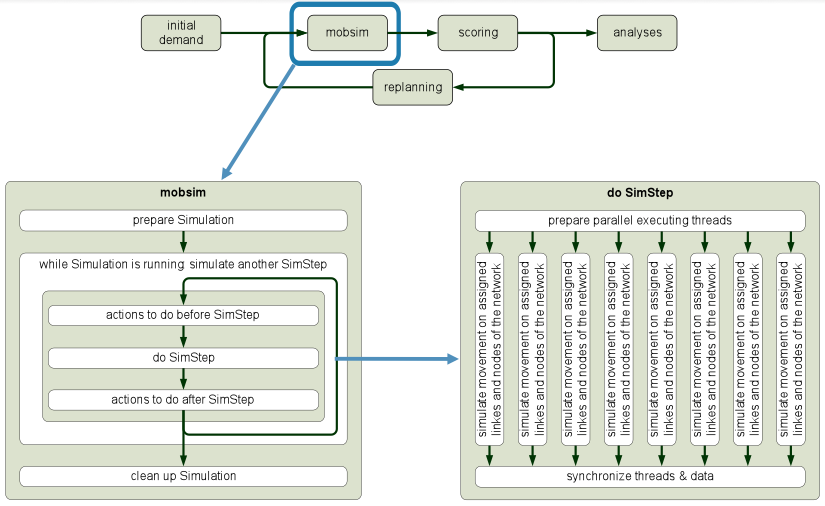
\includegraphics[width=\textwidth]{figures/qsimParallel/parallelqsim.png}
\caption{Design of the parallel qsim}
\end{figure}

The config option presumably is:
\begin{lstlisting}
<module name="qsim">
   ...
   <param name="numberOfThreads" value="5"/>
</module>

\end{lstlisting}

Any number of threads larger than $1$ triggers the use of the parallel version.

\umbruch
%%%%%%%%%%%%%%%%%%%%%%%%%%%%%%%%%%%%%%%%%%%%
%%%%%%%%%%%%%%%%%%%%%%%%%%%%%%%%%%%%%%%%%%%%
\subsection{"lanes". Status: works}

\authorsOfDoc{Dominik Grether}
\maintainers{Dominik Grether}
\authorsOfCode{Dominik Grether}

Make sure you read
\\ \small{\url{http://svn.vsp.tu-berlin.de/repos/public-svn/publications/vspwp/2012/12-03/}}
\\
before you use the lanes module to understand effects on the queue model.

\subsubsection{Configuration}

To use lanes make sure that the following parameters are set

\begin{lstlisting}{language=xml}
<module name="controler" >	
	...
	<param name="enableLinkToLinkRouting" value="true" />
	<param name="mobsim" value="qsim" />
	...
</module>

<module name="qsim" >
	...
	<param name="numberOfThreads" value="1" />
	...
</module>

<module name="scenario" >
	...
	<param name="useLanes" value="true" />
	...
</module>

<module name="network" >
	...
	<param name="laneDefinitionsFile" value="PATH TO FILE" />
	...
</module>
\end{lstlisting}


\subsubsection{Capacity interpretation of lanes}

In principle a lane is similar to the representation of a link in the queue model. 

The (exit) flow capacity of a lane is:

\begin{lstlisting}
capacity_value_of_lane / flow_capacity_factor
\end{lstlisting}

where
\begin{itemize}
	\item the capacity value of the lane is given in the laneDefinitions\_v2.0.xsd compatible input file
	\item the flow capacity factor is given in the qsim config group
\end{itemize}

The storage capacity of a lane is

\begin{lstlisting}
(length_of_lane * no_of_represented_lanes / effective_cell_size) * storage_capacity_factor
\end{lstlisting}

where
\begin{itemize}
	\item the length of the lane is calculated by the value of the \verb$<startsAt meterFromLinkEnd=10 />$ element within the \verb$<lane>$ element of the laneDefinitions\_v2.0.xsd file format. \\
		\begin{itemize}
			\item If the lane ends at the end of the link, its length is simply the \verb$meterFromLinkEnd$ value
			\item If the lane leads to other downstream lanes, its length is calculated from the distance between the position on the link the downstream lanes start from and the \verb$meterFromLinkEnd$ value of the lane. 
		\end{itemize}
	\item the number of represented lanes is the value of the \verb$number$ attribute of the  \verb$<representedLanes>$ element of the laneDefinitions\_v2.0.xsd file format.
	\item the storage capacity factor is given in the qsim config group
\end{itemize}


\umbruch
%%%%%%%%%%%%%%%%%%%%%%%%%%%%%%%%%%%%%%%%%%%%
%%%%%%%%%%%%%%%%%%%%%%%%%%%%%%%%%%%%%%%%%%%%
\subsection{"signalsystems". Status: works}

\authorsOfCode{Dominik Grether}
\maintainers{Dominik Grether}
\authorsOfDoc{Dominik Grether}

The signal systems module provides functionality to simulate traffic  lights with MATSim. It is recommended to use a nightly build that is  younger than 04-19-2011, i.e. revision 15081.

Have a look at the tutorial at \href{http://matsim.org/node/732}{http://matsim.org/node/732}.

The starting point of the technical documentation is
\begin{itemize}
	\item \href{http://www.matsim.org/javadoc/org/matsim/signalsystems/package-summary.html}{http://www.matsim.org/javadoc/org/matsim/signalsystems/package-summary.html}
\end{itemize}

Note that there are links to continuative documentation at the bottom of the package-summary.html www page.

MATSim ships with a tutorial that shows you how to set up a traffic  light scenario. The network and traffic light configuration of the  turorial is shown in the slides attached to this page. The network and  code can be found in the folder  tutorial/unsupported/example90TrafficLights in the nightly build. The  code examples are divided into several classes:
\begin{itemize}
	\item CreateSimpleTrafficSignalScenario.java: Uses traffic signals  without lanes and creates the traffic lights at nodes 3, 4, 7 and 8.
	\item CreateTrafficSignalScenarioWithLanes.java: Uses traffic signals with lanes and creates the traffic lights at nodes 2 and 5.
\end{itemize}



Publications using this module:
\begin{itemize}
	\item \href{https://svn.vsp.tu-berlin.de/repos/public-svn/publications/vspwp/2008/08-24/}{https://svn.vsp.tu-berlin.de/repos/public-svn/publications/vspwp/2008/08-24/}
	\item \href{https://svn.vsp.tu-berlin.de/repos/public-svn/publications/vspwp/2011/11-12/}{https://svn.vsp.tu-berlin.de/repos/public-svn/publications/vspwp/2011/11-12/}
	\item \href{https://svn.vsp.tu-berlin.de/repos/public-svn/publications/vspwp/2011/11-08/}{https://svn.vsp.tu-berlin.de/repos/public-svn/publications/vspwp/2011/11-08/}
\end{itemize}This documentation is missing an  explanation of the "lanes" option. Please ask if you need this  (separate "lanes" for separate turning movements).



%%%\includegraphics{User%27s%20Guide_files/application-pdf.png}\href{http://www.matsim.org/uploads/384/signals_tutorial_0.pdf}{signals\_tutorial.pdf} & 77.72 KB
%%\end{tabular}

\umbruch
%%%%%%%%%%%%%%%%%%%%%%%%%%%%%%%%%%%%%%%%%%%%
%%%%%%%%%%%%%%%%%%%%%%%%%%%%%%%%%%%%%%%%%%%%
\subsection{"transit" (public transport).  Status: works}

\authorsOfCode{Marcel Rieser}
\maintainers{Marcel Rieser}
\authorsOfDoc{Marcel Rieser}

A  public transport system is simulated and integrated on a fine scale  with both the traffic simulation and the behavior of the artificial  population.

Agents who use transit determine a route to their destination based  on the transit schedule. Transit vehicles are moved on the road network  in accordance with the traffic flow model, i.e. they may get stuck in  congestion and fail to keep their schedule. Agents getting on and off  transit vehicles cause realistic delays.

A transport mode decision model is implemented which allows agents to  switch their choice of driving a car or using transit based on the  relative utility of the two modes. The disutility of travel time, which  this model takes into account, is based on actual travel times taken  from the simulation.

See the \href{http://matsim.org/docs/tutorials/transit}{tutorial}. This requires quite some additional input.

\subsubsection{Reference}

M. Rieser, K. Nagel; \textbf{Combined agent-based simulation of private car traffic and transit}; IATBR 2009

\umbruch
%%%%%%%%%%%%%%%%%%%%%%%%%%%%%%%%%%%%%%%%%%%%
%%%%%%%%%%%%%%%%%%%%%%%%%%%%%%%%%%%%%%%%%%%%
\section{"JDEQSim".  Status: works}

\authorsOfCode{Rashid Waraich}
\maintainers{Rashid Waraich}
\authorsOfDoc{Rashid Waraich}

\subsubsection{Overview}

JDEQSim (Java Deterministic Event Driven Queue Based Simulation) has the following properties and features:
\begin{itemize}
	\item it is based on a discrete event simulation model
	\item traffic simulation is based on a queue model for streets (FIFO: first in first out)
	\item deadlock prevention is achieved by squeezing vehicles
	\item gaps  generated at front of queue propagate backwards with a speed called  'gapTravelSpeed' resulting in a more realistic traffic model
\end{itemize}

\subsubsection{Usage}

Insert  a new module called 'JDEQSim' into the config XML file. All parameters  are optional and have default values (shown below), never the less it  could be helpful to know their meaning and physical units.
\begin{lstlisting}{language=XML}
<module name="JDEQSim">
    <param name="endTime" value="00:00:00"   />
    <param name="flowCapacityFactor" value="1.0"   />
    <param name="storageCapacityFactor" value="1.0"   />
    <param name="minimumInFlowCapacity" value="1800"   />
    <param name="carSize" value="7.5"   />
    <param name="gapTravelSpeed" value="15.0"   />
    <param name="squeezeTime" value="1800"   />
</module>
\end{lstlisting}

The mobsim type now  also needs to be defined in the controler section of the config  file. See comments in config dumps in logfiles.

The  'endTime' defines the time of the last event of the simulation. If it is  set to '00:00:00', no end time is defined and the simulation will stop,  when the last event of the simulation has been processed. The (scaling)  parameters  'flowCapacityFactor' and 'storageCapacityFactor' can  be used as with mobSim and have no unit. The 'minimumInFlowCapacity'  defines for all roads the minimum number of cars, which could enter the  road per hour, for the congestion less case. The 'carSize' parameter  allows to set the size of a car in meters. The 'gapTravelSpeed'  parameter defines the speed of gaps in [m/s]. Finally the 'squeezeTime'  is used for deadlock prevention and defines, how long a car should wait  at maximum for entering the next road before deadlock prevention is  turned on (unit: seconds).

The 'minimumInFlowCapacity' is a  parameter, which was not published in the C++ DEQSim, but only used  interally and was hardcoded to the value 1800 vehicles per hour. This  value was estimated from literature assuming that independently from the  speed limit of a road the minimum interval between two vehicles is 2  seconds (inverse of 1800 vehicles per hour). This factor does not need  to be changed, when the 'flowCapacityFactor' is changed, as the scaling  is automatically done internally. The reason for publishing this factor  is to make it possible for users to adapt this factor, if they want to  use a different minium inflow capacity based on their model estimations.

\subsubsection{Hints}
\begin{itemize}
	\item You might consider turning on the module  'parallelEventHandling' when using JDEQSim, as often JDEQSim can make  much better use of this module than QueueSim (as JDEQSim is faster).
	\item If you are getting lots of breakdowns, consider using smaller squeezeTime (e.g. 10 seconds or lower)
\end{itemize}

\subsubsection{Requirements for the Plans XML File}

\begin{itemize}
	\item For each person the 'end\_time' of the first act must be defined ('dur' is ignored).
	\item For the other acts of a person either 'dur' or 'end\_time' needs to be defined
	\item If both 'dur' and 'end\_time' are defined, then only the one which occurs earlier is considered
\end{itemize}

\subsubsection{Differences between MobSim and JDEQSim}
\begin{itemize}
	\item QueueSim  uses a simulation approach called 'fixed-increment time advance'  instead of 'next-event time advance', which makes it much slower than  JDEQSim for high resolution networks.\footnote{%
%
I am sceptic if this statement is correct: QSim goes through all active links, which means that short empty link are also not considered by the QSim.  I would instead expect that the difference is rather for long links ($=$ low resolution networks), in conjunction with few vehicles (e.g.\ small sample sizes). kai, oct'13
%
}
	%%\item JDEQSim allows  squeezing of vehicles to resolve possible deadlocks. Deadlock prevention  in QueueSim is (traditionally) dealt with by removing vehicles from the  network or squeezing.
%
% squeezing has been possible in the qsim for many years now. kai, oct'13
	\item JDEQSim models gap travel times more realistically than QueueSim, where this feature is missing.
\end{itemize}




\subsubsection{Further Reading}

This implementation is based on the micro-simulation described in the following paper:

Charypar, D., K. Nagel and K.W. Axhausen (2007) An event-driven queue-based microsimulation of traffic flow, \emph{Transportation Research Record}, \textbf{2003}, 35-40.Order \href{http://trb.metapress.com/content/j2118065485r4611/?p=4f63e25a261d48d99eeebea19b494e24&amp;pi=0}{here}.

Some  Java specific implementation aspects and performance tests of JDEQSim  and parallelEventHandling are described in the following paper:

Waraich,  R., D. Charypar, M. Balmer and K.W. Axhausen (2009) Performance  improvements for large scale traffic simulation in MATSim, paper  presented at the \emph{9$^th$ Swiss Transport Research Conference}, Ascona, September 2009. Download from \href{http://www.ivt.ethz.ch/vpl/publications/reports/ab565.pdf}{here}.

\umbruch
%%%%%%%%%%%%%%%%%%%%%%%%%%%%%%%%%%%%%%%%%%%%
%%%%%%%%%%%%%%%%%%%%%%%%%%%%%%%%%%%%%%%%%%%%
\section{``simulation''. Status: deprecated as of sep/2014}

\sout{This  was essentially the production of the queue simulation until Nov/2010.  The "qsim" was then forked out for further development. Unfortunately,  this fork was done somewhat too late, so "simulation" is not exactly the  stable version that was used over many years, but something that is  already somewhat modified, and was not used very much after that.  (Please let us know if you have problems.)}

\sout{Note that you will get a "simulation" section in the log file even if  you have selected a different mobsim (such as qsim or jdqsim).}

\umbruch
%%%%%%%%%%%%%%%%%%%%%%%%%%%%%%%%%%%%%%%%%%%%
%%%%%%%%%%%%%%%%%%%%%%%%%%%%%%%%%%%%%%%%%%%%
\section{External mobsim.  Status: unknown}

\authorsOfCode{Marcel Rieser}
%\maintainers{C. Dobler, IVT}
\authorsOfDoc{Kai Nagel}


There used to be an option to start an external mobsim. This still seems to be there but the syntax is a bit awkward:
\begin{lstlisting}
<module name="controler" >
   ...
   <param name="mobsim" value="null" />
</module>
<module name="simulation" >
   <param name="externalExe" value="<path-to-executable>" />
</module>


\end{lstlisting}

I.e.\ you need to specify that you are \emph{not} using the (queue)Simulation, but then set a parameter inside the (queue)Simulation config block.

I (kn, oct'13) cannot say if this is still working.  

\umbruch
%%%%%%%%%%%%%%%%%%%%%%%%%%%%%%%%%%%%%%%%%%%%
%%%%%%%%%%%%%%%%%%%%%%%%%%%%%%%%%%%%%%%%%%%%

\chapter{Other configurable modules}

% I now think that there should be
% * matsim containers (population, network, facilities, households, ...)
% * mobsims
% * other
% kai, oct'13



Modules are loosely defined by their corresponding entry in the config file.

They are also sorted in the same sequence (which is done by the machine, not by content).

Note that individual config options are often explained inside the config section of the log file.

Config file modules that just define files/directories are, as a tendency, not explained here.Note that strategy modules (such as ReRoute, Planomat) are described in a separate section.

Maintainers are mentioned as far as possible, but they are \emph{not} responsible for answering arbitrary service requests.

\umbruch
%%%%%%%%%%%%%%%%%%%%%%%%%%%%%%%%%%%%%%%%%%%%
%%%%%%%%%%%%%%%%%%%%%%%%%%%%%%%%%%%%%%%%%%%%
\section{"global". Status: indispensable}

\maintainers{Marcel Rieser}

"Global" information. Arguably should be merged with "controler" section.

\umbruch
%%%%%%%%%%%%%%%%%%%%%%%%%%%%%%%%%%%%%%%%%%%%
%%%%%%%%%%%%%%%%%%%%%%%%%%%%%%%%%%%%%%%%%%%%
\section{"controler". Status: indispensable}

\authorsOfCode{Marcel Rieser}
\maintainers{Marcel Rieser}
\authorsOfDoc{Marcel Rieser}

\subsubsection{Javadoc}

\href{http://www.matsim.org/javadoc/org/matsim/core/controler/package-summary.html}{www.matsim.org/javadoc/org/matsim/core/controler/package-summary.html}



\subsubsection{Config Parameters}

\href{http://www.matsim.org/javadoc/org/matsim/core/controler/package-summary.html#controler_parameters}{www.matsim.org/javadoc/org/matsim/core/controler/package-summary.html\#controler\_parameters}


\subsubsection{In Brief}

Central module to run matsim. Specifies, for example, the number of iterations.



%%\subsubsection{Notes}

%%See \href{http://matsim.org/node/398}{here} for some instructions how to use an external executable as mobsim.

% the reference is wrong, and there is a separate section on this in the present (latex) manual, which should be sufficient.

\umbruch
%%%%%%%%%%%%%%%%%%%%%%%%%%%%%%%%%%%%%%%%%%%%
%%%%%%%%%%%%%%%%%%%%%%%%%%%%%%%%%%%%%%%%%%%%
% I think this is now fully a contrib.  kai, oct'13
%%\section{"evacuation"(-ivt). Status: ??}

%%Evacuation code used by IVT; please note that IVT and VSP use different evacuation codes.

%%Maintained by C. Dobler.

%%I (kn) don't know how this works

%%\umbruch
%%%%%%%%%%%%%%%%%%%%%%%%%%%%%%%%%%%%%%%%%%%%
%%%%%%%%%%%%%%%%%%%%%%%%%%%%%%%%%%%%%%%%%%%%
% I think this is now fully a contrib.  kai, oct'13
%%\section{"evacuation"(-vsp). Status: works if you know what you are doing}

%%(Note that VSP and IVT use different evacuation packages.)

%%\subsubsection{\textbf{Maintenance and Questions}}

%%G. Lämmel, TU Berlin

%%\subsubsection{\textbf{Javadoc}}

%%\href{http://www.matsim.org/javadoc/org/matsim/evacuation/package-summary.html}{http://www.matsim.org/javadoc/org/matsim/evacuation/package-summary.html}


%%\subsubsection{\textbf{\textbf{Config Parameters{}}}}

%%\href{http://www.matsim.org/javadoc/org/matsim/evacuation/package-summary.html#evacuation_parameters}{http://www.matsim.org/javadoc/org/matsim/evacuation/package-summary.html\#evacuation\_parameters}

%%\subsubsection{\textbf{\textbf{In Brief}}}

%%I (kn) can't say how this works. There is, at this point, neither documentation nor funding.

%%\umbruch
%%%%%%%%%%%%%%%%%%%%%%%%%%%%%%%%%%%%%%%%%%%%
\section{"parallelEventHandling". Status: works for ivt and vsp}

\authorsOfCode{Rashid Waraich}
\maintainers{Rashid Waraich}

see details \href{http://matsim.org/node/238}{here}.



\umbruch
\section{"planCalcScore". Status: nearly indispensible}

\maintainers{Marcel Rieser}

This module contains the definitions for the utility function.

Some help for it should be in the tutorials.

There is also some description in the "scoring function" section of the documentation.

\umbruch
%%%%%%%%%%%%%%%%%%%%%%%%%%%%%%%%%%%%%%%%%%%%
%%%%%%%%%%%%%%%%%%%%%%%%%%%%%%%%%%%%%%%%%%%%
\section{"strategy". Status: indispensable}

\maintainers{Marcel Rieser}

See \href{http://matsim.org/node/478}{here}.

\umbruch
%%%%%%%%%%%%%%%%%%%%%%%%%%%%%%%%%%%%%%%%%%%%
%%%%%%%%%%%%%%%%%%%%%%%%%%%%%%%%%%%%%%%%%%%%
\section{"travelTimeCalculator". Status: nearly indispensable}

\maintainers{Marcel Rieser}

"router" and "travelTimeCalculator" are separate in matsim, so that  they can be configured separately. They refer to each other,  though.

\umbruch
%%%%%%%%%%%%%%%%%%%%%%%%%%%%%%%%%%%%%%%%%%%%
%%%%%%%%%%%%%%%%%%%%%%%%%%%%%%%%%%%%%%%%%%%%
\section{"vspExperimental". Status: used by VSP}

\authorsOfCode{Kai Nagel}
\maintainers{Kai Nagel}
\authorsOfDoc{Kai Nagel}

This  section defines switches that are used at VSP or when collaborating  with VSP. There are experimental and may we withdrawn without notice.

%%Of particular interest are some defaults that everybody at VSP should be using. These can be switched on by:
%%\begin{lstlisting}
%%<module name="vspExperimental" >
%%   <param name="vspDefaultsCheckingLevel" value="abort" />
%%   ...
%%</module>

%%\end{lstlisting}

%%This will make the code abort when these defaults are violated.

%%The number of VSP defaults will grow over time. This may have  the effect that some config file that used to be working for you in the  past may not work any more after an svn update. I will try to  communicate such changes, but will sometimes fail to do so. In any  case, if you encounter an abort because of a vsp defaults violation,  please
%%\begin{itemize}
%%	\item check what is causing the problem, and
%%	\item enter the relevant config setting into all config files that you use.
%%\end{itemize}

%%If you think that you cannot live with these settings, please talk to me.

%%Since those settings involve all aspects of matsim, they may often be irrelevant to you. Please set them anyways.

\umbruch
%%%%%%%%%%%%%%%%%%%%%%%%%%%%%%%%%%%%%%%%%%%%
%%%%%%%%%%%%%%%%%%%%%%%%%%%%%%%%%%%%%%%%%%%%
%%\section{Deprecated modules}

%%%%%%%%%%%%%%%%%%%%%%%%%%%%%%%%%%%%%%%%%%%%
%%%%%%%%%%%%%%%%%%%%%%%%%%%%%%%%%%%%%%%%%%%%
%%\subsection{"world"}

%%\textbf{Dismantler:} Michael Zilske

%%This was an attempt to integrate GIS functionality into matsim.

%%Has been superceeded by calls to geotools. Please use geotools  functionality. Look under the demand generation tutorials for  getting some ideas.

%%World also provides datastructures to assign facilities to links, and  links to zones, etc. This functionality is mostly used in initial  demand modelling, but is not very straight-forwardly implemented. Should  be replaced in the future with some kind of "mappig manager" to manage  the mappings between different MATSim objects, like facilities, links,  etc.
%%%%%%%%%%%%%%%%%%%%%%%%%%%%%%%%%%%%%%%%%%%%
%%%%%%%%%%%%%%%%%%%%%%%%%%%%%%%%%%%%%%%%%%%%

There are two visualizers available for MATSim. The original, open source 
visualizer is \href{http://matsim.org/docs/extensions/otfvis}{OTFVis}, which is
a MATSim extension. It requires current OpenGL drivers. The source code is 
available, so you can add your own information visualization code. On the 
other hand, there is currently little support for it from our part.

Then there is Via, a commercial visualizer developed by Senozon. It  has more
features, a better UI, and it is more stable. On the other hand, it visualizes
output files from simulation runs, whereas OTFVis runs in the same VM as
MATSim and can peek into the running simulation.

The supported way of programming your own data analysis or visualization code
is to analyze MATSim output in the form of Events, either reading in the 
events.xml file, or writing an EventHandler and receiving Events programmatically.

\section{Senozon Via}

Via can be obtained from the \href{http://senozon.com/products/via}{Senozon website}.
While the application is commercial, a limited version is available freely from the website. 
A brief introduction to using Senozon Via is part of the "Learning MATSim in 8 Lessons"
tutorial in the \href{http://www.matsim.org/docs/tutorials/8lessons/getting-started}{Getting Started} lesson.

Via is able to visualize most of MATSim's data (network, agent plans, transit schedule, facilities, counts)
along additional data (e.g. shape files, GPS traces).
It allows to analyze and visualize the outcome of MATSim simulations by loading the generated events-file.


On the relation between Senozon (a private company), Senzon Via (a commercial software), 
MATSim (an open source project/software) and MATSim OTFVis (an open source software):
\begin{itemize}\styleItemize
	\item Historically, MATSim is open source. An important reason for this was that multiple teams contribute, and we wanted to make progress rather than sorting out the intellectual property.
	\item However, this community is unable to provide support for any and all requests that may come up. As a result, the commercial company \href{http://www.senzon.com/}{Senozon} was founded by two long-time MATSim developers, which provides commercial support for such situations.
	\item Senozon also helps significantly with the development and maintenance of the MATSim core. The open source community and Senozon have a shared interest in a functional and robust MATSim core: Both our academic research and Senozon's commercial success depend on this.
	\item In addition, Senozon has developed the \href{http://senozon.com/products/via}{MATSim visualization and analysis software Via}.  OTFVis remains available but maintenance is limited. In  particular, please understand that we are unable to provide support for specific hardware configurations or specific query requests.
\end{itemize}

\section{Events analysis}

In  order to write MATSim events handlers, some amount of Java programming  is necessary. Material can thus found in the api-users section of the documentation, see \href{http://www.matsim.org/node/17}{here}.

\authorsOfDoc{Marcel Rieser, Johan W. Joubert}

\bigskip

%%\begin{chapter-intro}
%%Some chapter intro.
%%\end{chapter-intro}

\section{Software}

MATSim runs on any machine that has the \href{http://java.sun.com/javase/downloads/index.jsp}{Java Platform, Standard Edition} (SE) 7 or newer installed (commonly referred to as ``Java 7" or newer).

\section{Hardware}

Smaller  scenarios (e.g. the examples included in the tutorials, 5\%- or  10\%-samples of large scenarios) can be run on common desktop or laptop  computers.

To simulate large scenarios (several hundreds of  thousands of agents, networks with ten-thousands of links and nodes),  high end computers with a large amount of memory (RAM) may be required  to keep the agents' data in memory. The description of agents' plans and  the simulation output can take several Gigabytes of hard disk space. To  store the data for several scenarios and / or output of simulation  runs, large amounts of disk space may thus be needed. MATSim can read  and write compressed files to reduce the amount of required disk space,  but this aspect still shouldn't be underestimated. MATSim can make use  of multiple CPUs or CPU cores that share common memory (``shared memory  machine'') during the replanning-phase.

Running large scenarios for  a high number of iterations can take several hours, up to a few days.  Thus it may be advisable to have a dedicated machine running MATSim if  you plan to simulate many different scenarios.

\subsection{Recommendations}
\begin{itemize}
	\item To try MATSim out:
\\Any modern laptop or desktop computer with 1GB RAM and 500MB free disk space should be suitable.
	\item To run a large scenario (100 000+ agents, networks with 50 000+ links): 
\\A high-end desktop computer with at least 4GB RAM and 200 GB free disk space.
	\item To run many large scenarios, so they can be compared against each other: 
\\Multiple high-end desktop computers or servers with at least 4GB RAM that share a common storage disk (at least 1TB).
\end{itemize}

The  high numbers for free disk space result from the fact that the  simulation writes quite a lot of data to the disk during a run. For  analysis, usually only the last version of the data is required, and  data from earlier iterations can be deleted, freeing space up again.

\subsection{What we use}

Currently,  we simulate most of our scenarios on machines with 16 or 32 GB RAM,  having 2 dual- or quad-core processors. The amount of memory allows us to run 2  scenarios at the same time on the machines. A \href{http://en.wikipedia.org/wiki/RAID}{RAID}  array is used as storage backend, offering about 4 TB of hard disk  space. This huge disk space is able to store the results of hundreds of  simulations and will suit us for the next few years. Computers and RAID  are regular components used in data centers, nowadays available at moderate prices.

\section{Benchmarks}

There are a few benchmark exercises you can consider in MATSim.

\subsection{Standard MATSim benchmarks}
\subsubsection{Overview}
The performance of MATSim depends on a lot of different factors:
\begin{itemize}
\item CPU-speed (although by far not always the limiting factor!)
\item Memory-Bus / -Controller (we're moving huge amounts of memory, the faster the better)
% \item Java Virtual Machine (JVM 1.7 is usually faster than JVM 1.6)
\item File system (local Hard drive vs. RAID vs. NFS vs \ldots)
\end{itemize}
To get a better understanding, under which circumstances MATSim performs best, we created a simple benchmark (performance test) that runs 20 iterations of a sample scenario with different settings. If you run the benchmark on your machine, we would be happy if you could send us your results.

\subsubsection{Download and installation}
Download the following zip-file: \href{http://matsim.org/files/benchmark/benchmark.zip}{benchmark.zip}{[35MB]}. Unzip the downloaded file.

\subsubsection{Running the benchmark}
On the command line, run the following:
\begin{lstlisting}{language=xml}
java -Xmx500m -jar Benchmark.jar
\end{lstlisting}
This will generate a directory output with some files in it from the run. The test will usually run between 25 and 40 minutes. The benchmark requires Java 1.5 or newer and 150MB free disk space. If you want to re-run the benchmark, rename or delete the \texttt{./output/} directory and run the test again.

\subsubsection{Submitting benchmark results}
Please send an email to \texttt{benchmark AT matsim DOT org} containing:
\begin{itemize}
\item the file \texttt{output/stopwatch.txt}
\item the file \texttt{output/logfile.log}
\item a description of your benchmark environment, including:
\begin{itemize}
\item vendor of machine (e.g. Sun, Dell, Apple, etc.)
\item processor-type (vendor (AMD, Intel, etc.), model-number, clock-speed, cache-size, number of processors and cores, \ldots)
\item memory (bus-speed, memory-controller, etc.)
\item storage system (rpm, cache size, \ldots, type: e.g. local hard drive, RAID, \ldots)
\item operation system
\item java virtual machine
\item any other information you think might be of interest to us
\end{itemize}
\end{itemize}

We collected some results and did a short analysis on them. Have a look at the results in the next section. If you want your results included as well or have some interesting findings yourself, please submit us your benchmark results.

\subsection{MATSim benchmark results}
The benchmark contains parts of the code running in parallel (the replanning part, using 4 threads) and other parts running single-threaded.

\subsubsection{Speed comparison}
The benchmark was run on some of our production servers with different versions of Java Virtual Machines. The servers have 2 Single-Core ``AMD Opteron Processor 248'' running at 2.2 GHz (date of purchase: fall 2004, so they have to be considered as \emph{old}). The Java Virtual Machines tested were:

\begin{description}
\item[IBM Java 5 64bit]\quad The default Java 5 version on the servers. The JVM identified itself as \texttt{J2RE 1.5.0 IBM J9 2.3 Linux amd64-64 j9vmxa6423ifx-20080811}
\item[Sun 6u5 64bit]\quad The default Java 6 version on the servers, identifying itself as \texttt{1.6.0\_05; Sun Microsystems Inc.; mixed mode; 64-bit}
\item[Sun 5u19 64bit]\quad The latest (as of writing this text) Java 5 version from Sun, Java 5 update 19 64-bit.
\item[Sun 5u19 32bit]\quad The latest Java 5 version from Sun, Java 5 update 19 32-bit.
\item[Sun 6u14 64bit]\quad The latest Java 6 version from Sun, Java 6 update 14 64-bit.
\item[Sun 6u14 32bit]\quad The latest Java 6 version from Sun, Java 6 update 14 32-bit.
\item[Sun 6u14 64bit COP]\quad Sun's Java 6 update 14 64-bit, started with the extra argument \texttt{-XX:+UseCompressedOops}. Compressed Object Pointers should "improve performance of the 64-bit JRE when the Java object heap is less than 32 gigabytes in size" (see \href{http://java.sun.com/javase/6/webnotes/6u14.html}{Java SE 6 Update 14 Release Notes}). As an additional advantage, memory consumption should also be a bit lower when using only 32bits for object pointers.
\item[Sun 6u14 64bit COP + AO]\quad Sun's Java 6 update 14 64-bit, started with the extra argument \texttt{-XX:+UseCompressedOops -XX:AggressiveOpts}. In addition to using Compressed Object Pointers, also try out the new \emph{experimental implementation} of \texttt{java.util.TreeMap} that can improve the performance as MATSim makes heavy use of TreeMaps (although not necessarily that often iterating over them)
\item[Sun 6u14 32bit AO]\quad Sun's Java 6 update 14 32-bit, started with the extra argument \texttt{-XX:AggressiveOpts}. Just for comparison, also start the 32-bit version of the JVM with the aggressive optimization option.
\end{description}

The shown number in Figure~\ref{fig:Benchmark01} are the average of two runs of the benchmark for each configuration (Yeah, two isn't that big a sample, we know... but it should still be valid to demonstrate some findings).
\begin{figure}[h]
\centering
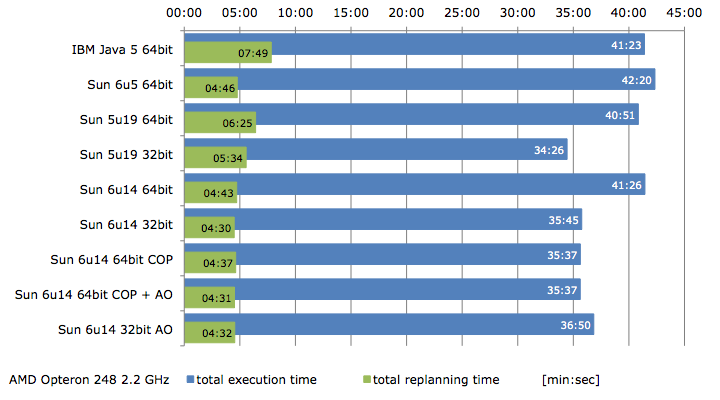
\includegraphics[width=0.75\linewidth]{figures/benchmarks/benchmark1}
\caption{The average of two runs of the benchmark for each configuration.}
\label{fig:Benchmark01}
\end{figure}
What can be observed is the huge difference of execution time in general between 32-bit and 64-bit versions of the virtual machines. The \emph{compressed object pointers} (COP) feature of Suns JVM 6u14 seems to compensate for this nicely, making the 64-bit version about the same speed than the 32-bit version. The aggressive optimization options (AO) on the other hand doesn't seem to influence the performance of MATSim drastically.

While the difference between Suns Java 5 and Java 6 versions in the total execution time seem more or less random, there seems to be a performance improvement for the multithreaded replanning part by changing from Java 5 to Java 6. Interestingly, despite IBM's worse multithreaded performance, it is able to catch up in the single-threaded parts to come in with a similar total execution time than Sun's 64-bit JVMs.

The benchmark was also run on other server machines:

\begin{itemize}
\item Servers with two Dual-Core AMD Opteron 2222 processors, running at 3.0 GHz; date of purchase winter 2007/2008 (very similar architecture than the previously tested AMD Opteron 248 systems, just \emph{newer} with higher clocked CPU).
\item Servers with Intel Xeon X5355 Quad-Core processors, clocked at 2.66 GHz, 8 MB L2 cache, built with 65 nm technology.
\item Servers with Intel Xeon E5430 Quad-Core processors, clocked at 2.66 GHz, 12 MB L2 cache, built with 45 nm technology.
\item Servers with Intel Xeon E5530 Quad-Core processors, clocked at 2.4 GHz, 8 MB L3 cache, 45 nm technology, Nehalem architecture.
\item Servers with Intel Xeon E7540 Hex-Core processors, clocked at 2.0 GHz, 18 MB L3 cache, 45 nm technology, Nehalem architecture, DDR3 RAM.
\end{itemize}
Comparing (in Figure~\ref{fig:Benchmark02}) the AMD servers running at 2.2 GHz and 3.0 GHz, the most obvious difference is the time for the replanning, explainable by the different number of cores the machines have. 
\begin{figure}[h]
\centering
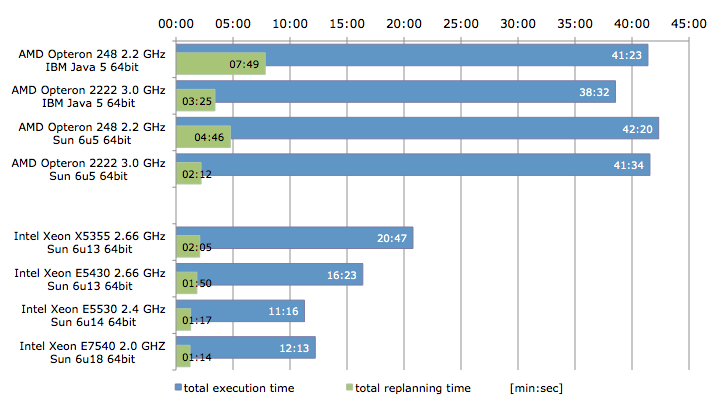
\includegraphics[width=0.75\linewidth]{figures/benchmarks/benchmark2}
\caption{The average of two runs of the benchmark for different servers.}
\label{fig:Benchmark02}
\end{figure}
Interestingly, the remaining execution time didn't really improve by the change in CPU speed, leading to the guess that the performance of the memory controller or the memory bus is limiting the speed of MATSim (both AMD servers seem to have a front side bus of 1000 MHz).

The Intel servers were massively faster than the AMD machines. We do not yet know if it's the different memory controller, faster memory bus, or if Sun's JDK is just more optimized for Intel processors. Anyway, the difference is striking. And each newer generation of Intel processors seems to deliver a real performance upgrade, even when running at a lower clock-speed.

At last, the benchmark was also run on some of our laptop machines: An Apple MacBook Pro with a Intel Core 2 Duo processor clocked at 2.33 GHz (model from fall 2006), running Mac OS X 10.5.7, and an IBM/Lenovo Laptop with the same Intel Core 2 Duo processor, 2.33 GHz, running a Gentoo 64-bit Linux (Kernel 2.6.28). Both laptops have a front side bus of 667 MHz, so from a technical view point they are very similar.

On the Apple MacBook Pro, the following Java Virtual Machines were used:

\begin{description}
\item[Apple JVM 5u16 32bit]\quad The default Java 5 version on Mac OS provided by Apple.
\item[Apple JVM 6u7 64bit]\quad The default Java 6 version on Mac OS provided by Apple.
\item[Soylatte 6u3 32bit]\quad An early port of OpenJDK 6, identifying itself as \texttt{1.6.0\_03-p3; Sun Microsystems Inc.; mixed mode; 32-bit}, provided by \href{http://landonf.bikemonkey.org/static/soylatte/}{Landon Fuller}.
\end{description}
On the Lenovo Laptop, an OpenJDK 6u0 64-bit JVM was used.
\begin{figure}[h]
\centering
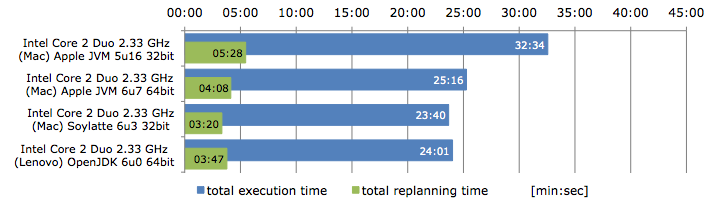
\includegraphics[width=0.75\linewidth]{figures/benchmarks/benchmark3}
\caption{The average of two runs of the benchmark for laptops.}
\label{fig:Benchmark03}
\end{figure}
Surprisingly, Apple pulled the trick to make their 64-bit Java 6 a lot faster than the older 32-bit Java 5—well, it could also mean that their Java 5 offering was just very slow\ldots The Mac-port of OpenJDK 6 (\emph{Soylatte}) is even a bit faster, but that may be likely due to the difference between 64-bit and 32-bit.

Are you able to run the MATSim benchmark even faster? Please tell us so! We're very interested in your benchmark results.

\subsubsection{Memory usage comparison}
MATSim writes out information about memory usage from time to time into the logfile. Plotting this information gives a jagged line running from left to right. Heights and lows in the plot can be explained with the Java Garbage Collector, only freeing up the memory from time to time. Still, one can guess the absolute minimum of memory required by MATSim by looking at the lower parts of the curve (that's then when a Garbage Collection just ran, showing all the memory that could not be collected).

Comparing the memory consumption in Sun's (currently) latest Java VM version holds no real surprises.
\begin{figure}[h]
\centering
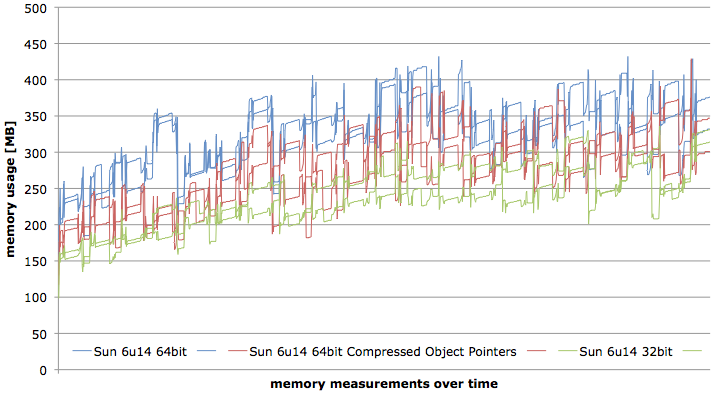
\includegraphics[width=0.75\linewidth]{figures/benchmarks/benchmark_memory}
\caption{Memory usage over iterations.}
\label{fig:Benchmark04}
\end{figure}

It can be clearly seen that the 64-bit JVM uses the largest amount of memory, due to the fact that each object pointer takes up 8 bytes. The 32-bit JVM uses the least memory. The 64-bit JVM with compressed object pointers seems to lie somewhere in between—although I would have expected it to be comparable to the 32-bit JVM, it seems that it still uses a bit more memory for unknown reasons. Anyway, it comes in handy to know that one can load now larger scenarios on a 32GB (or less) machine. The memory savings, compared to a 64-bit JVM without compressed object pointers, should be even bigger the larger the scenario is or the more details the simulated network has, so this feature really looks promising.
 
So, by how much can you improve your MATSim simulation's performance?

\section{Speeding up your own MATSim runs}
There are a few things you can try to speed up your simulation runs. The following hints are not in any specific order.%% {\color{red}(are they?)}.

\subsection{Use an up-to-date Java version}
Java 7 usually performs better than Java 6.

\subsection{Use compressed object pointers in 64-bit JVM}

Since Sun Java 6, Update 14, if you use a 64-bit JVM and use at most 32 GB of RAM, start Sun's Java virtual machine with the argument 
\begin{lstlisting}{language=xml}
-XX:+UseCompressedOops
\end{lstlisting}
This reduces the size of object pointers to 32 bit, making many pointer operations a lot faster than when they were 64 bit long, while still supporting heap sizes larger than 2 GB (what a regular 32-bit JVM would do). See the \href{http://www.oracle.com/technetwork/java/javase/6u14-137039.html}{Java SE 6 Update 14 Release Notes} for more details. In addition, we observed notable speed-ups in the region of 10\% in the run time of MATSim. Since Java SE 6 Update 23 and in Java 7, this option is enabled by default.

\subsection{Parallelization}
When running a MATSim simulation, unused cores can be utilized to make the simulation faster. There are now three ways to improve performance using parallelization, and each can be switched on or off separately.

\subsubsection{Event handling}\label{sec:ParallelEventsHandling}
The event handler which is used by default, is running in the same thread as the simulation. For this reason, you can switch on parallel event handling by adding the \texttt{parallelEventHandling} module to the MATSim \texttt{Config} XML file as follows:
\begin{lstlisting}{language=xml}
<module name="parallelEventHandling">
    <param name="numberOfThreads" value="1" />
</module>
\end{lstlisting}
The only required parameter in this module is \texttt{numberOfThreads}. The value of this parameter specifies how many threads (cores) should be assigned to handling events.

There is an additional optional parameter \texttt{estimatedNumberOfEvents}, which can be optimized to your simulation resulting in slightly faster runs. But its usage requires an estimate of the number of events which will occur in one iteration.
\begin{lstlisting}{language=xml}
<param name="estimatedNumberOfEvents" value="5000000" />
\end{lstlisting}
The following are some hints to consider and pitfalls to avoid:
\begin{itemize}
\item Don't make any  assumptions on the order, in which the handlers are executed (as they are executed in parallel).
\item Don't write the data in one handler and read that data in a different handler. Although this is possible, special care is required as synchronization between threads is needed for this. Furthermore this could lead to a degradation of the speed up.
\item There is no point in using parallel event handling, if you have just one core available on your machine.
\item Always make sure, that one thread is needed for the single cpu simulation. This means, if you have 4 cores, you can set the parameter 'numberOfThreads' to maximum 3.
\item If 2 handlers have been added to the simulation, then there is no point in assigning 3 threads to parameter \texttt{numberOfThreads}, because it won't make the simulation faster (but rather could slow it down in some cases).
\item The number of handlers can be bigger than \texttt{numberOfThreads}. In this case automatically if possible, each thread is assigned the same number of handlers. 
\item If the simulation is quite slow (compared to event handling), you won't be able to make full use of parallel event handling.
\end{itemize} 
The actual speed up you get depends on many factors, especially on those in the aforementioned hints and pitfalls. Experiments on a 16 core machine with different numbers of handlers have shown that the parallel event handler can reduce the simulation time with a very low overhead. Some Java specific implementation aspects of \emph{JDEQSim} and the \texttt{parallelEventHandling} module are described in the paper by Waraich, R., D. Charypar, M. Balmer and K.W. Axhausen (2009) Performance improvements for large scale traffic simulation in MATSim, paper presented at the 9th Swiss Transport Research Conference, Ascona, September 2009. This paper can be downloaded \href{http://www.ivt.ethz.ch/vpl/publications/reports/ab565.pdf}{here}. 

\subsubsection{Mobility simulation}\label{sec:ParallelQsim}
\authorsOfCode{C. Dobler, IVT}
\maintainers{C. Dobler, IVT}

There is a parallel version of the qsim. Analysis of performance and structure of (non parallel) qsim shows:
\begin{itemize}
\item Simulation of movement on links and over nodes is most time consuming.
\item Within a timestep actions on nodes and links can be simulated on parallel threads with low additional synchronization effort.
\end{itemize}

The parallel qsim is based on the existing qsim and can be used by just adding a new parameter to a scenario configuration file (see ). First performance measurements show promising results, and a working paper will be published in Q2 2010. A structural description of the parallel qsim is shown in Figure~\ref{fig:ParallelQsim}.
\begin{figure}[htp]
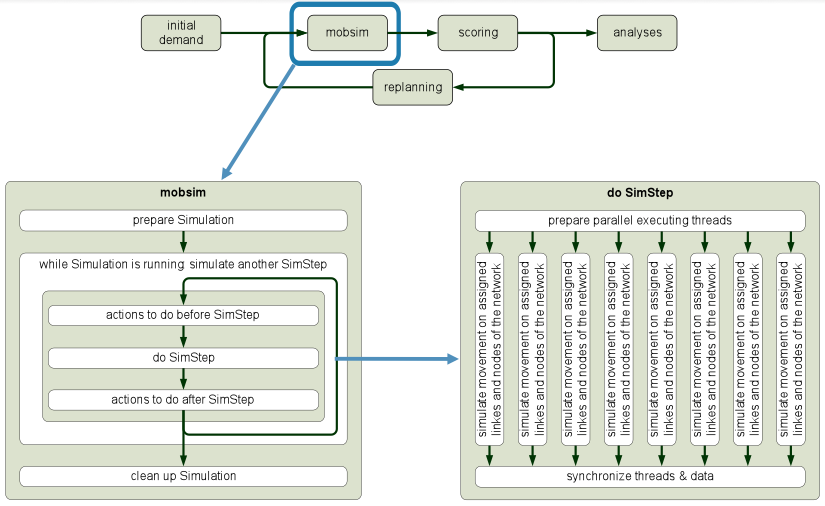
\includegraphics[width=\textwidth]{figures/qsimParallel/parallelqsim.png}
\caption{Design of the parallel qsim.}\label{fig:ParallelQsim}
\end{figure}

To activate it, ensure that a \texttt{qsim} module is added to the config XML file of MATSim, and set the \texttt{numberOfThreads} parameter as follows:
\begin{lstlisting}{language=xml}
<module name="qsim">
   ...
   <param name="numberOfThreads" value="5"/>
</module>
\end{lstlisting}
or however many number of threads you want to use. An unlimited number of threads will \emph{not} make your simulation run infinitely fast. A performance \emph{decrease} can actually occur, depending on the scenario size. Refer to Christoph Dobler's thesis (Chapter 5) for a complete discussing in this regard. Figure~\ref{fig:QsimPerformance} shows an estimation of the (optimal) number of threads required for a given scenario size (expressed as number of events generated).
\begin{figure}[h]
\centering
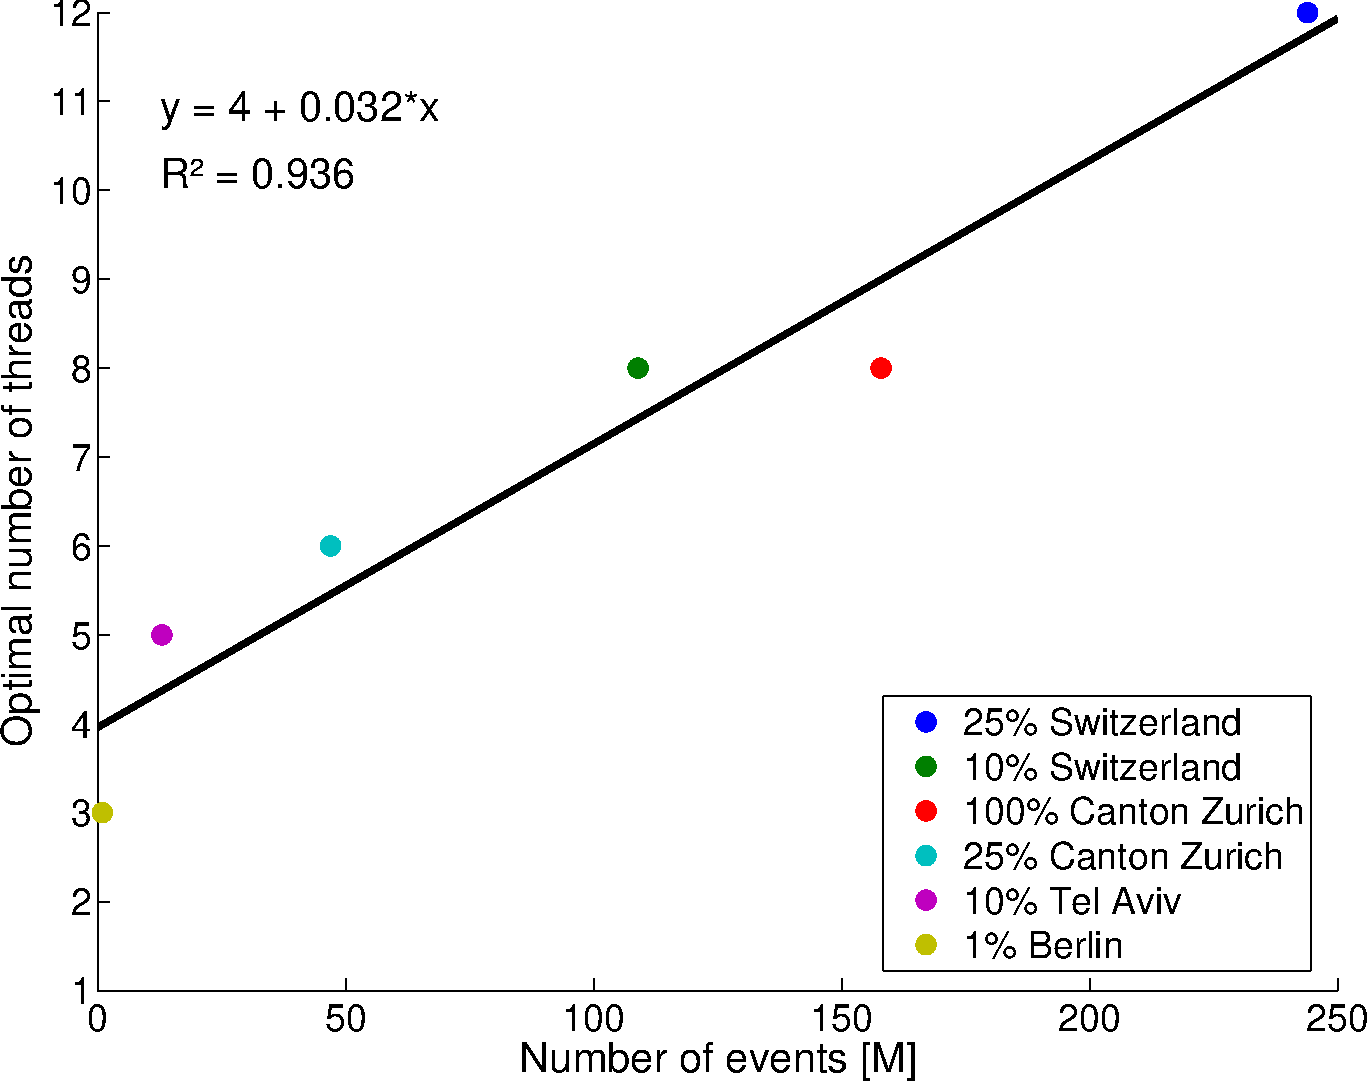
\includegraphics[width=0.6\linewidth]{figures/benchmarks/EventsVsSpeedUp}
\caption{Estimated number of threads to use for a given scenario size.} 
\label{fig:QsimPerformance}
\label{figureLabel}
\end{figure}

Dobler, C. (2013). Travel behaviour modelling for scenarios with exceptional events --- methods and implementations, Dissertation, IVT, ETH Zurich, Zurich. Available online \href{http://e-collection.library.ethz.ch/view/eth:7633}{here}.

\subsubsection{Replanning}
To set the simulation to parallelize the replanning phase, the following parameter must be set the the \texttt{global} module of the config XML file:
\begin{lstlisting}{language=xml}
<module name="global">
  ...
  <param name="numberOfThreads" value="8" />
</module>
\end{lstlisting}

\subsection{Limit the writing of events}
Writing the simulation events to files in each iteration not only consumes a lot of disk space, but also a considerable amount of time. Add the following parameter to your configuration to restrict writing events to certain iterations:
\begin{lstlisting}{language=xml}
<module name="controler">
  ...
  <param name="writeEventsInterval" value="10" />
</module>
\end{lstlisting}

\subsection{Use faster routing algorithms}
By default, MATSim uses a routing algorithm based on Dijkstra's shortest path algorithm. But MATSim also includes a faster routing algorithm, based on the A$^{\star}$ algorithm with landmarks. To use this routing algorithm, add the following configuration parameter to your configuration file:
\begin{lstlisting}{language=xml}
<module name="controler">
  ...
  <param name="routingAlgorithmType" value="AStarLandmarks" />
</module>
\end{lstlisting}

\subsection{Comparing parallelisation options}
The following shows two different benchmarks using jdeqsim (Section~\ref{sec:Jdeqsim}), parallel events handling (Section~\ref{sec:ParallelEventsHandling}), or both. The first benchmark, Figure~\ref{fig:JdeqsimTime}, uses the ivtch-osm network (approximately 60,000 links), while the second one, Figure~\ref{fig:JdeqsimTime-navteq}, uses a navteq network with much more links.

\subsubsection{QueueSim versus JDEQSim using parallel events handling}
Zrh 10\%, ivtch-osm network; computing times per iteration (computer = cluster4 = 2x ``Dual-Core AMD Opteron Processor 2222'', 3.0 GHz, 1000 MHz FSB).  Runs 669, 676, 678, 679
\begin{figure}[h]
\centering
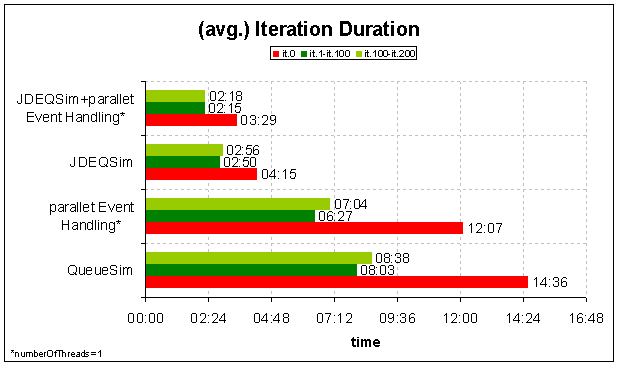
\includegraphics[width=0.75\linewidth]{figures/benchmarks/jdeqsimtime}
\caption{Using the ivtch-osm network.}
\label{fig:JdeqsimTime}
\end{figure}

Computing times per Iterations.  Scenario = navteq network of Switzerland; computer = cluster4 = servers with 2x ``Dual-Core AMD Opteron Processor 2222'', 3.0 GHz, 1000 MHz FSB.
\begin{figure}[h]
\centering
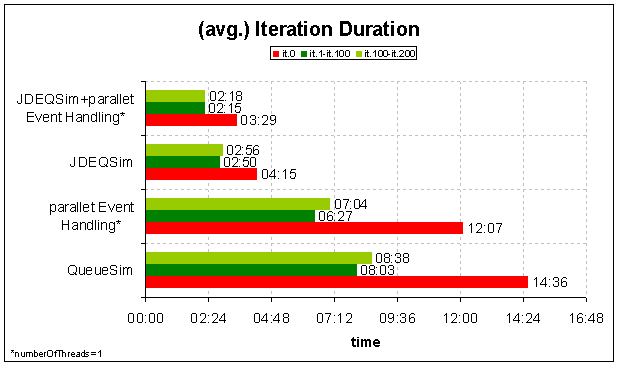
\includegraphics[width=0.75\linewidth]{figures/benchmarks/jdeqsimtime}
\caption{Using the ivtch-osm network.}
\label{fig:JdeqsimTime-navteq}
\end{figure}


\NextFile{PolicyMeasures.html}
\chapter{Policy Measures}

A discussion of policy measures that can be investigated with matsim is under \href{http://matsim.org/policy-measures}{matsim.org/policy-measures}  . It is not in the user section but in the developer section of  the documentation since, at this point, many of those measures need  additional coding. Clearly, something like adding or removing lanes or  links can be investigated without any coding.


% no longer include extensions into user guide, decided at devmtg2013. mr/oct13
%\NextFile{UsingExtensions.html}
\chapter{Using MATSim Extensions}

\subsubsection{Introduction}

The default MATSim releases contain all the functionality typically  used to model agent behavior and simulate traffic. But sometimes, this  just is not enough. The MATSim Extensions provide additional  functionality for specific tasks, and can be used along MATSim. \href{http://www.matsim.org/extensions}{MATSim Extensions}  gives an overview of the currently available extensions. Please note  that these extensions are usually provided and maintained by single  persons from the community, and thus long-term support may vary from the  default MATSim release.

\subsubsection{Downloading Extensions}

All extensions come as a compressed zip-file. You can either download  the last stable release of an extension to be used together with the  stable release of MATSim, or you can download a so-called "nightly  build"—an automatically created, but untested and probably unstable  version of the extension.
\begin{itemize}
	\item You can download the stable releases of extensions from \href{http://sourceforge.net/projects/matsim/files/MATSim/}{SourceForge}.
	\item Likely unstable nightly builds can be downloaded from our \href{http://matsim.org/files/builds/}{nightly builds directory}.
	\item Make sure to also download MATSim itself. The extensions cannot be used without MATSim.
\end{itemize}

\subsubsection{Using Extensions on the Command Line}

Once you've downloaded an extension and MATSim, unzip the extension  and place the extension's directory inside the MATSim directory, next to  the 
\texttt{libs} directory. The file/directory structure should look similar to the following example:
\begin{verbatim}
matsim/
+ MATSim.jar
+ libs/
| + $<$lots of .jar files$>$
+ extension1/
| + extension1.jar
+extension2/
| + extension2.jar
| + libs/       $<$-- not all extensions contain additional libs
| | + $<$one or more .jar files$>$
\end{verbatim}

Then, start your simulation with the extension.jar-file on the classpath along the MATSim jar-file, e.g:
\begin{verbatim}
java -Xmx512m -cp MATSim.jar:extension1/extension1.jar:extension2/extension2.jar org.matsim.run.Controler myConfig.xml


\end{verbatim}

On Windows, use 
\texttt{;} instead of 
\texttt{:} to separate the different jar-files.

\subsubsection{Using Extensions in Eclipse}

Unzip the downloaded extension and place the extension's directory in  your eclipse project. Then, add the extension's jar-file to the 
\texttt{Java Build Path} in Eclipse's 
\texttt{Project Settings}.

\subsubsection{Documentation about Specific Extensions}

Extensions are developed and documented by their maintainers. Not all extensions are listed below; see the \href{http://www.matsim.org/extensions}{list of available} extensions for their description and documentation.



\vfill\eject
\NextFile{GTFS2TransitSchedule.html}
\section{GTFS2TransitSchedule}

This guide whill show you how to convert GTFS data to a MATSim Transit Schedule

\subsubsection{Automatic conversion}
\begin{itemize}
	\item Put the set of GTFS files of each public transport system in a different folder of your file system.
	\item Create a java program that constructs an object of the class
\texttt{GGTFS2MATSimTransitSchedule}in the package 
\texttt{GTFS2PTSchedule} which is part of this extension.For this you need to specify:
\end{itemize}
\begin{enumerate}
	\item An array of folders (
\texttt{File} class) where your public transport system specifications are located.
	\item An array of Strings representing the network modes correspondent to each public transport defined in b) (e. g. “
\texttt{car}” for buses, “
\texttt{rail}” for metro).
	\item The MATSim network object with the nodes in latitude and longitude coordinates (
\texttt{WGS84}).
	\item An array of Strings with the names of the calendar services that are desired (e. g. “
\texttt{weekday}”, “
\texttt{daily}”). Remember that MATSim only simulates one day, but the GTFS files specify routes for many calendar days or dates.
	\item The desired output coordinates system
\end{enumerate}
\begin{itemize}
	\item Call the method 
\texttt{TransitSchedule getTransitSchedule()}.  Then, each route of each given public transit systems will be processed  with the semi-automatic procedure presented in the following figure.
\end{itemize}
\begin{figure}[htp]
	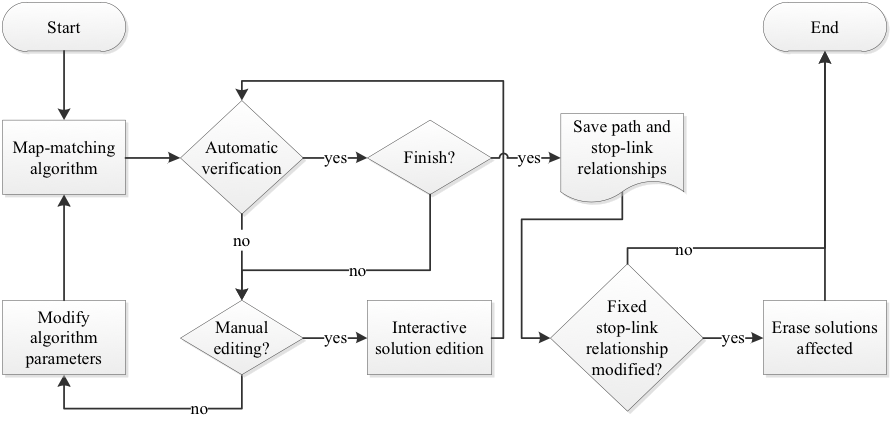
\includegraphics{figures/gtfs2schedule/gtfsAutoConversion.png}
\end{figure}




\subsubsection{Manual correction of automatic conversion}

For the manual editing process one can visualize, edit and verify the solution for each route:
\begin{itemize}
	\item Visualization: A navigation network is displayed, including all  relevant information for working with one single route. This includes  the route’s profile, the given sequence of GPS points and its current  solution (path and stop-link relationships). Selected elements are drawn  in a different color. All is displayed in a bi-dimensional interactive  way with refresh of the cursor location in the working coordinates, and  panning,  zoom and view-all options.
	\item Selection: Different options for selecting elements of the solution  or elements from the network are provided. It is possible to select the  nearest link (solution or network), nearest node (network) or nearest  stop (solution) to a point indicated by the user. When a stop that has a  stop-link relationship already, the corresponding link is selected as  well. If a link of the solution path is selected and it does not have a  subsequent link connected, a new one from the network is selected with  one click; the selected link is the one with the most similar angle than  the line defined by the end node of the initial link and a point  indicated by the user.
	\item Solution modification: The first link of the sequence can be added  selecting any link of the network. If a link of the solution path does  not have a subsequent link connected, it is possible to add one  according to the selection function described in (b). If there are two  subsequent links in the solution that are not connected (a gap), a  subsequence that connects the mentioned links is added, using the  shortest path algorithm, with the current parameters. Furthermore,  selecting one link of the path, it is possible to delete it, or to  delete all the links before or after it. Finally, stop-link  relationships can be modified selecting both elements. If the modified  relationship was fixed, the user  is prevented because the tool erase  the solutions of the routes to which the selected stop belongs.
	\item Network modification: New nodes to the road network can be added. In  addition, with any node selected, it is possible to add a new link  selecting the end node.
\end{itemize}

Hints and interaction details:
\begin{itemize}
	\item It is necessary to pass the verification process (“Is OK”) for saving a route result
	\item The routes are saved in temporal files located in the ./data/paths/ folder relative to the program location.
	\item Panning and zoom functions are provided dragging the mouse and moving the mouse wheel.
	\item View all function is provided typing the “v” key
	\item Up and down keys allow to select the next or previous link of the path.
	\item “$<$” or ”$>$” keys allow to select the previous or next stop 

\begin{figure}[htp]

\end{figure}
	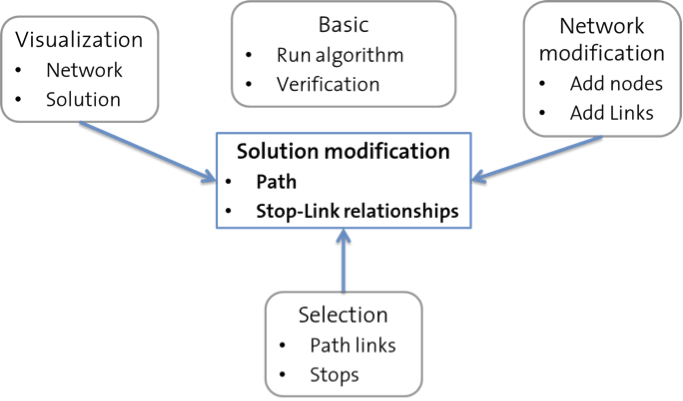
\includegraphics{figures/gtfs2schedule/gtfsManualEdit.png}
\end{itemize}

\subsubsection{Saving the converted data}

Finally, after the semi-automatic process, the Transit Schedule  object is returned and the network object is modified (splitting, new  nodes and links, and modes of the links). One can save in a XML  the 
\texttt{TransitSchedule} object constructing a 
\texttt{TransitScheduleWriter} object, and the modified network with a 
\texttt{NetworkWriter}.


\vfill\eject
\NextFile{MATSim4UrbanSim.html}
\section{MATSim4UrbanSim}

\subsection{Guide on UrbanSim usage of the travel model plug-in}

The current travel model plug-in implementation is applicable for the  Brussels zone, Zurich parcel, PSRC (Puget Sound Region Council) parcel  and Seattle parcel UrbanSim application.

Note that some of the instructions may change since the travel model plug-in is still under development.

\subsubsection{1 Prerequisites}

You must have installed UrbanSim, before getting started with the  travel model plug-in. The following provides an entry point to install  UrbanSim and continues with installation instructions for additional  software packages required by the travel model plug-in.

\subparagraph{Hints for installing UrbanSim}

To install UrbanSim please follow the UrbanSim Downloads and Installation Instructions on \href{http://urbansim.org/Download/}{http://urbansim.org/Download/}.

When installing OPUS and UrbanSim manually you can get the  installation instructions in "Downloading Sample Data and Source Code"  on: \href{http://urbansim.org/Download/DownloadingSampleDataAndSourceCode}{http://urbansim.org/Download/DownloadingSampleDataAndSourceCode}.

Windows users using the installer are getting the source code and data automatically.

Finally make sure that all UrbanSim environment variables, meaning  OPUS\_HOME, OPUS\_DATA\_PATH and PYTHONPATH, are set as described in the  installation instructions, see \href{http://urbansim.org/Download/SixtyFourBitMachines}{http://urbansim.org/Download/SixtyFourBitMachines} for Windows, \href{http://urbansim.org/Download/MacintoshInstallation}{http://urbansim.org/Download/MacintoshInstallation} for Mac or \href{http://urbansim.org/Download/LinuxInstallation}{http://urbansim.org/Download/LinuxInstallation} for Linux.

Note:  For using the travel model plug-in it is sufficient only to install the  required Python packages, i. e. numpy, scipy, lxml, sqlalchemy and  elixir.

\subparagraph{MATSim4UrbanSim prerequisites}

In addition to the UrbanSim installation the MATSim travel model plug-in requires the following software installed:
\begin{itemize}
	\item Java JDK 1.6 or newer: Download and install the newest version  of the Java SE Development Kit (JDK) for your operating system from \href{http://www.oracle.com/technetwork/java/javase/downloads/index.html}{http://www.oracle.com/technetwork/java/javase/downloads/index.html}. Make sure adding Java's /bin directory to the PATH environment variable. Click\href{http://java.com/en/download/testjava.jsp}{here}to test ifjavaisalready installed on your computer.
	\item Python XML Schema Bindings (PyXB): Download the PyXB 1.1.3 distribution file from \href{http://sourceforge.net/projects/pyxb/files/pyxb/1.1.3/}{http://sourceforge.net/projects/pyxb/files/pyxb/1.1.3/}  and extract it to a convenient place. Open a command prompt (Windows)  or a terminal (Mac, Linux). To install PyXB (this may requires  administrator or root privileges) go into the extracted directory and  type
\\


\texttt{python setup.py install}
\end{itemize}

\subsubsection{2 MATSim4UrbanSim installation}

This section describes how to install MATSim4UrbanSim.

\subparagraph{Automatic installation}

Make sure to have the Python lib directory included to the  PYTHONPATH. The Python lib directory is the directory that contains the  site-package directory that is already included in the PYTHONPATH. The  lib directory should be something like


\texttt{C:$\backslash$Python2.6$\backslash$Lib$\backslash$ }for Windows,


\texttt{/Library/Frameworks/Python.framework/Versions/2.6/lib/} for Mac or


\texttt{/usr/lib/python2.6/} for Linux (Ubuntu).

To install MATSim4UrbanSim open command prompt (Windows) or a  terminal (Mac, Linux) and navigate to opus\_matsim/configs in the opus  source directory. Than type


\texttt{python install\_matsim4urbansim.py}

This creates the subdirectories matsim4opus/jar, loads required  MATSim executables and libraries and configures them. After the  installation the file/directory structure should look something like  Figure 1.

To test whether the MATSim4UrbanSim installation was successful follow the instructions described in Section 2.3.

Note: The installer will replace jar-files and libraries from a previous MATSim4UrbanSim installation.

\subparagraph{Manual installation}

In case that the automatic installation does not work follow these instructions:
\begin{itemize}
	\item Create the following directory structure in OPUS\_HOME: OPUS\_HOME/matsim4opus/jar
	\item Download the following files from \href{http://www.matsim.org/files/builds/}{http://www.matsim.org/files/builds/} into the jar directory:   
\begin{itemize}
	\item MATSim\_rXXXXX.jar (where XXXXX refers the current revision)
	\item MATSim\_libs.zip
	\item matsim4urbansim-X.X.X-SNAPSHOT-rXXXXX.zip (where XXXXX refers the current revision)
\end{itemize}
	\item Rename MATSim\_rXXXXX.jar into "matsim.jar".
	\item Extract the zip files MATSim\_libs.zip and matsim4urbansim-X.X.X-SNAPSHOT-rXXXXX.zip. After that the zip files can be removed.
	\item Rename the directory matsim4urbansim-X.X.X-SNAPSHOT-rXXXXX into  "contrib". Than navigate into contrib and rename the jar-file  matsim4urbansim-X.X.X-SNAPSHOT.jar into "matsim4urbansim.jar".
\end{itemize}

Be careful when renaming files or directories (i. e. make sure  that everything is written in lower case and check for spelling errors).  After the installation the file/directory structure in the matsim4opus  directory should look something like Figure 1. To test whether the  MATSim4UrbanSim installation was successful follow the instructions  described in Section 2.3.

\subparagraph{Test your MATSim4UrbanSim installation}

To test your installation open a command prompt (Windows) or a  terminal (Mac, Linux) and navigate to opus\_matsim/tests in the opus  source directory (PYTHONPATH). Then type


\texttt{python travel\_model\_test.py}

This starts a test scenario. If the test completes without errors, your travel model plug-in should be working.

\begin{figure}[htp]
\includegraphics[width=\textwidth]{figures/matsim4urbansim/structure.png}
\caption{After the installation the matsim4opus directory should contain the depicted files and subdirectories.}
\end{figure}

\subsubsection{3 Using MATSim for UrbanSim}

This section aims to explain the MATSim travel model plug-in at the example of the Seattle\_parcel scenario.\textbf{}

\subparagraph{MATSim Data Requirements}

MATSim related input-files are:
\begin{itemize}
	\item a road network in MATSim format (mandatory)
	\item a plans file (optional)
\end{itemize}

These files are not included in the UrbanSim base\_year\_data and  must be added manually. To store these files create the red marked  folder structure as shown in Figure 2. This means store network files in  the "matsim/network" folder and the plans-files in the "matsim/plans"  folder.

For the current Seattle parcel example scenario you can download the zipped matsim folder \href{https://svn.vsp.tu-berlin.de/repos/public-svn/matsim/examples/countries/us/seattle/matsim.zip}{here.}  Unzip it into your OPUS\_DATA/seattle\_parcel/base\_year\_data/2000/  directory. After that your seattle\_parcel base\_year\_data should look  like Figure 2.

\begin{figure}[htp]
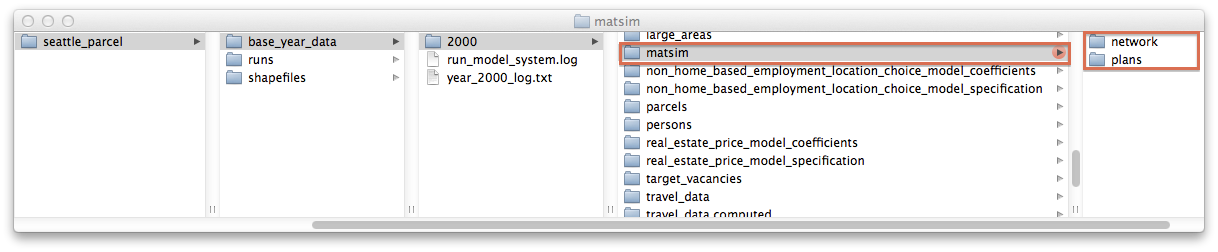
\includegraphics[width=\textwidth]{figures/matsim4urbansim/seattle_parcel_base_year_dir_v2.png}
\caption{Store MATSim related files like road networks and  plans-files directly in the base\_year\_data folder of the corresponding  UrbanSim application.}
\end{figure}

\subparagraph{UrbanSim Data Requirements}

In order to create input data for MATSim UrbanSim requires certain  data sets and attributes to reflect where a person lives and works.

\textbf{For UrbanSim parcel} applications the following data sets and attributes (in parenthesis) are required:
\begin{itemize}
	\item persons (person\_id, household\_id, job\_id)
	\item households (household\_id, building\_id)
	\item jobs (job\_id, building\_id)
	\item buildings (building\_id, parcel\_id)
	\item parcels (parcel\_id, x\_coord\_sp, y\_coord\_sp, zone\_id)
	\item zones (zone\_id)
\end{itemize}

\textbf{For UrbanSim zone} applications the following data sets and attributes (in parenthesis) are required:
\begin{itemize}
	\item persons (person\_id, household\_id, job\_id)
	\item households (household\_id, zone\_id)
	\item jobs (job\_id, zone\_id)
	\item zones (zone\_id, xcoord, ycoord)
\end{itemize}

\subparagraph{Travel Model Configuration Options}

In a recent effort a set of MATSim configuration parameters are  embedded into the travel\_parameter\_configuration section of the UrbanSim  configuration. This allows to configure MATSim in the OPUS GUI under  the Models tab as shown in Figure 3. The travel model conguration  section consists of a few lines of XML code and can be added into  existing UrbanSim configurations. A sample configuration for Seattle  parcel including the travel model configuration section can be  downloaded \href{https://svn.vsp.tu-berlin.de/repos/public-svn/matsim/examples/countries/us/seattle/seattle_parcel.xml}{here}.

\begin{figure}[htp]
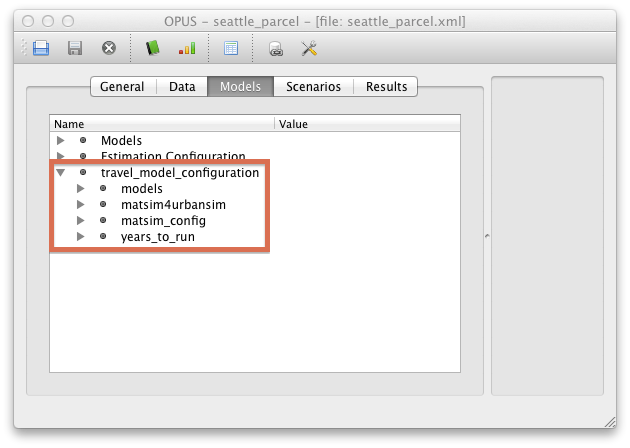
\includegraphics[width=\textwidth]{figures/matsim4urbansim/gui.png}
\caption{MATSim4UrbanSim configuration in OPUS GUI}
\end{figure}

The following explains step by step the MATSim configuration options provided by the OPUS GUI.

Launch the OPUS GUI and open the Seattle\_parcel sample configuration  (download see above). Switch to the Models tab to get to the travel  model configuration section as shown in Figure 4. The following  subsections are available:

\textbf{Models}:

The models section contains five models that couple MATSim with UrbanSim:
\begin{enumerate}
	\item \textbf{get\_cache\_data\_into\_matsim\_parcel} generates the MATSim input for UrbanSim parcel applications
	\item \textbf{get\_cache\_data\_into\_matsim\_zone} generates the MATSim input for UrbanSim zone applications
	\item \textbf{run\_travel\_model\_parcel }executes MATSim for UrbanSim parcel applications.
	\item \textbf{run\_travel\_model\_zone} executes MATSim for UrbanSim zone applications.
	\item \textbf{get\_matsim\_data\_into\_cache} imports the results of the traffic simulation for the next UrbanSim iteration (no distinction between parcel and zone here).
\end{enumerate}

To run MATSim for parcel applications enable the models \textbf{1},\textbf{ 3} and \textbf{5}. For UrbanSim zone applications use the models \textbf{2, 4} and \textbf{5}.

\textbf{MATSim4UrbanSim}:
\begin{itemize}
	\item \textbf{population\_sampling\_rate}: The population  sampling rate determines the percentage of considered travellers for a  MATSim run. For instance 0.01 means that only 1\% of travellers are  considered for the traffic simulation. This option allows to speed up  computations on the MATSim side by using low sampling rates, e.g. for  testing purposes.
\\   Note that low sampling rates cause some peculiarities in terms of  realism. In this situation results are useful for sketch planning only,  not for quantitative analysis. Higher sampling rates need more ram, hard  drive space and computation time.
	\item \textbf{matsim\_controler}: This determines which access-  and accessibility measures to perform in MATSim and accordingly which  UrbanSim data sets and attributes to update. Following options are are  available:   
\begin{itemize}
	\item \textbf{zone\_to\_zone\_impedance}: This returns an  origin-destination-matrix (OD-matrix) compromising car (congested and  free speed), bicycle and walk travel times at the mornig peak hours and  vehicle trips for each pair of zones. The resulting OD-matrix is  imported into the "travel\_data" data set in UrbanSim.
	\item \textbf{agent\_performance}: The agent performance  feedback contains the individual travel performances of MATSim agents  including congested car travel times and travel distances for commuting  from home to work and back.
\\     Note: To update the travel performances of all UrbanSim persons use a  full population\_sample\_rate, i.e. the population\_sampling\_rate must be  1. The resulting values are imported into the "persons" data set in  UrbanSim.
	\item \textbf{zone\_based\_accessibility}: This measures the  accessibility to work places at the zone-level for the modes car (free  speed and congested), bicycle and walk. Such accessibility values are  attached (or updated) to the zones data set in UrbanSim. The resulting  accessibilities are imported into the "zones" data set in UrbanSim.
	\item \textbf{cell\_based\_accessibility: }This measures the  accessibility to work places at the parcel-level for the modes car (free  speed and congested), bicycle and walk. The resulting accessibilities  are imported into the "parcels" data set in UrbanSim.
\end{itemize}
	\item \textbf{controler\_parameter}: This section is for configuring the cell\_based\_accessibility measure:   
\begin{itemize}
	\item \textbf{cell\_size}: This parameter sets the cell size  (in meter) and thus the resolution of the cell\_based\_accessibility  measure, see Figure 4. Short side lengths lead to higher resolutions,  but also to longer computation times.
	\item \textbf{shape\_file} (optional): To speed up accessibility  computation the exact shape, i.e. a boundary like in Figure 4, of the  study area can be provided asshape file(optional). Make sure that the shape-file is consistent with the UrbanSim coordinates.
	\item \textbf{bounding\_box }(optional): To speed up  accessibility computation the study area can be defined by a bounding  box giving the most top, left, right and bottom coordinates (optional).  Make sure that these are consistent with the UrbanSim coordinates.
\\     To use the bounding box enable the "use\_bounding\_box" option and putthe coordinatesinto the correspondingfields, e.g. put the most top coordinate into the "baounding\_box\_top" field.
\end{itemize}
\end{itemize}

By  default neither a shape file nor a bounding box is needed. In this case  MATSim takes the road network to determine the study area, which could  need more ram and computation time for accessibility computation.

\begin{figure}[htp]
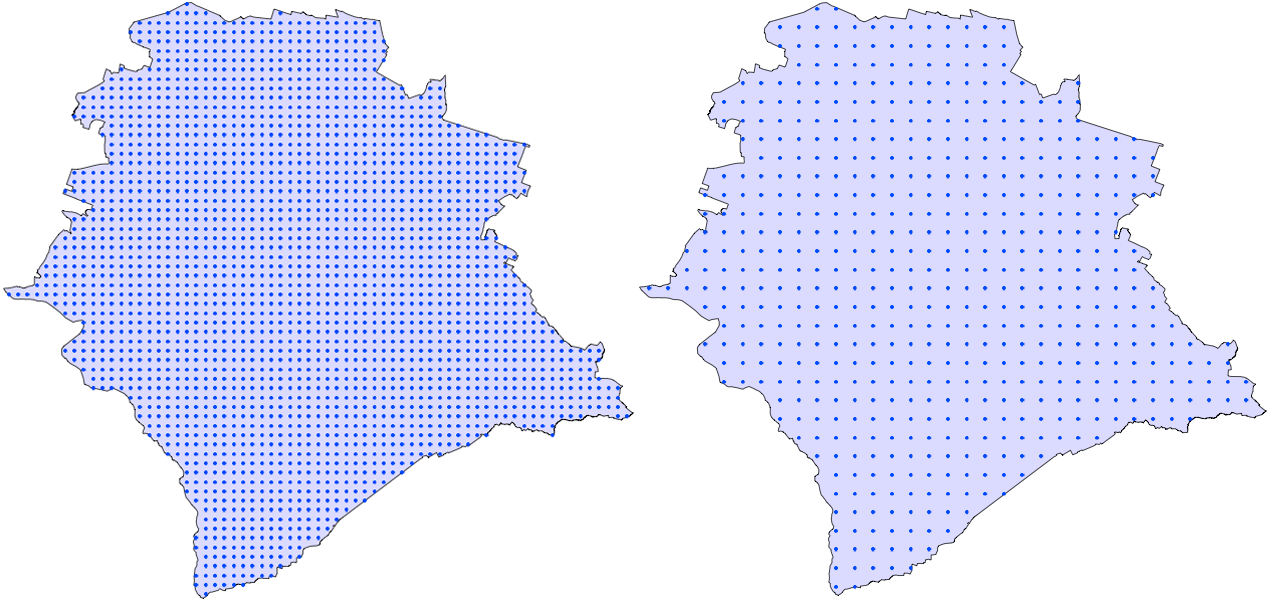
\includegraphics[width=\textwidth]{figures/matsim4urbansim/resolution.png}
\caption{The figure visualizes how the study area (blue area) is  subdivided into cells of configurable size by using the "cell\_size"  parameter. The left illustration has a side length of 200 meter  (cell\_size=200), the right illustration has a side length of 400 meter  (cell\_size=400). The blue dots are the corresponding cell centroids,  which serve as measuring points for the accessibility computation.}
\end{figure}

\begin{itemize}
	\item \textbf{accessibility\_parameter}: At this point the marginal utilities e.g. for different transport modes can be configured (\sout{for calibration instructions see \href{http://www.matsim.org/node/650}{here}} no this has nothing to do with calibration. kn, apr'13]]):   
\begin{itemize}
	\item \textbf{accessibility\_destination\_sampling\_rate}: This  determines the percentage of considered opportunities, currently work  places, for the accessibility computation. A value of 1 is recommended.
	\item \textbf{use\_MATSim\_parameter}: Enables MATSim default settings for the following parameter:     
\begin{itemize}
	\item \textbf{use\_logit\_scale\_parameter\_from\_MATSim}: This sets the logit scale parameter to a MATSim default value (currently this is 1.0)
	\item \textbf{use\_car\_parameter\_from\_MATSim}: This sets the marginal utility for traveling by car (beta$_tt,car$) to a MATSim default value (currently -12 utils/h). Otherwise the car\_parameter settings (see below) are used.
	\item \textbf{use\_walk\_parameter\_from\_MATSim}: This sets the marginal utility for traveling on foot (beta$_tt,walk$) to a MATSim default value (currently -12 utils/h). Otherwise the walk\_parameter settings (see below) are used.
	\item \textbf{use\_raw\_sums\_without\_ln}: If enabeld the summation of the term exp(V$_ik$) is computed, i.e.accessibility is computed as A$_i$:=sum$_k$( exp(V$_ik$) ) for all opportunities k.
\end{itemize}
	\item \sout{\textbf{logit\_scale\_parameter}: Set a custom value for the logit scale parameter. Make sure that "use\_logit\_scale\_parameter\_from\_MATSim" is disabled!}


((this functionality is currently disabled. It is not clear if the  following parameters should refer to the best path computed by matsim  (according to a different utility function), or if they should compute a  new best path according to that new utility function (where, however,  congested would not be equilibrated). kn, apr'13)) 

\sout{\textbf{car\_parameter} and \textbf{walk\_parameter}}: This allows to configure the disutility of traveling V$_ik,mode$ for a given mode (car, bicycle, walk) and thus to configure the accessibility measurement. V$_ik,mode$ is composed as follows:

%%V$_ik,mode$:= V$_ik,tt,mode$ + V$_ik,tt$^2$mode$ + V$_ik,ln(tt),mode$ + V$_ik,td,mode$ + V$_ik,td$^2$mode$ + V$_ik,ln(td),mode$ + V$_ik,m,mode$ + V$_ik,m$^2$mode$ + V$_ik,ln(m),mode$

     where "tt" are travel times, "td" are travel distances and "m" are monetary costs.

     Each summand $V_ik,xx,mode$ consists of the following contributions, see Figure 5:
\begin{enumerate}
	\item \sout{The disutility of travel of reaching the transport network from origin \emph{i}. It is assumed that opprotunities (e.g. work places) can only be reached via the transport network.}
	\item \sout{The disutiliy of travel on the network towards opportunity \emph{k}}
	\item \sout{The disutility of travel reaching opportunity \emph{k} from the transport network}
\end{enumerate}
\end{itemize}
\end{itemize}

\sout{As a result the disutility V$_ik,xx,mode$ is composed as follows:}

\sout{V$_ik,xx,mode$:= beta$_xx,wlk$* xx$_wlk,gap,i $+ beta$_xx,mode$ * XX$_mode$ + beta$_xx,wlk$ * xx$_wlk,gap,k$
\\
\\  where xx refers to the travel costs (tt, tt$^2$,ln(tt), td, td$^2$,ln(td), m, m$^2$,ln(m)) and beta$_xx,wlk$ and beta,$_xx,mode $are marginal utilities that convert the given travel cost into utils.
\\
\\  Setting the marginal utility beta$_xx$ to zero removes the corresponding summand from the equation. In order to use your own V$_ik,mode$  make sure that the corresponding switches  ("use\_car\_parameter\_from\_MATSim" and/or  "use\_walk\_parameter\_from\_MATSim") are disabled.}

\begin{figure}[htp]
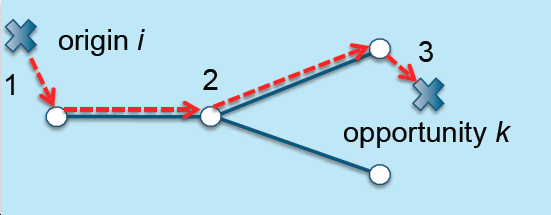
\includegraphics[width=.5\textwidth]{figures/matsim4urbansim/vik.png}
\caption{The composition of the disutility V$_ik,xx,mode $consists  of three parts: the cost (1) to reach network from i, (2) the cost on  the network and (3) the costs to reach the opportunity \emph{k} from the network.}
\end{figure}

\begin{itemize}
	\item \textbf{random\_location\_distribution\_radius\_for urbansim\_zone}:  This option is only relevant for UrbanSim zone applications. It  randomly distributes persons living in a certain zone within a given  radius (in meter) around the zone centroid. See also section 4  "Additional MATSim4UrbanSim Parameters" for an alternative distribution  of persons.
\end{itemize}

\begin{figure}[htp]
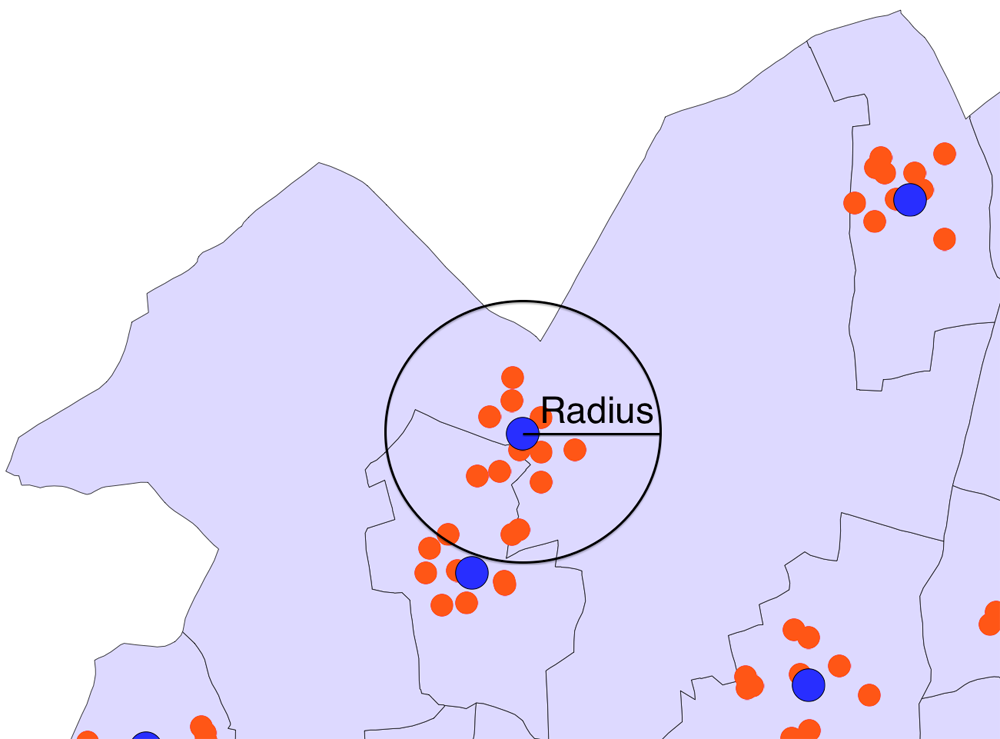
\includegraphics[width=\textwidth]{figures/matsim4urbansim/radius.png}
\caption{The random\_location\_distribution\_radius\_ for\_urbansim\_zone  parameter randomly distributes persons (red dots) living in a certain  zone within a given radius around the zone centroid (blue dot).}
\end{figure}


\textbf{MATSim Config}:

Thissectioncontainsparametersfor theconfigurationof thetrafficmodel.
\begin{itemize}
	\item \textbf{common}: The common subsection provides some basic configuration options for MATSim   
\begin{itemize}
	\item \textbf{external\_MATSim\_config}: This allowsto integratean external MATSim configuration for a specified UrbanSim year by setting the relative path to the separate configuration file, which must be located in the OPUS HOME directory.
\\Note  that overlapping parameter settings are overwritten by the external  configuration such as the population sampling rate, network, last  iteration, input plans file, plan calc score and strategy parameters (if  defined in both, the MATSim4UrbanSim and external MATSim config).
\\     Previously, parameter settings made in the external conguration were overwritten.
\\
\\     In order to set an external configuration file add the following  lines in the "travel\_model\_configuration $>$ matsim\_config $>$ common"  section:
\\
\begin{verbatim}
<external_matsim_config type="dictionary">
  <matsim_config name="2001" type="file">relative_path/to/external_matsim_config.xml</matsim_config>
</external_matsim_config>}
\end{verbatim}
	\item \textbf{matsim\_network\_file}: This points, as the name  implies, to a road network in MATSim format. A relative path (located in  the OPUS\_HOME directory) to the network file is expected.
	\item \textbf{last\_iteration}: This gives the number of MATSim iterations to perform. In MATSim iterations start at zero.
	\item \textbf{input\_start\_plans\_file}: This gives the path to a  “relaxed” plans file from which MATSim starts ("warm start"). It allows  MATSim to recycle agent decisions like route and departure times from a  previous run to speed up computing time. If this is not set, MATSim  will construct its initial plans file purely from UrbanSim input, and  take much longer to relax ("cold start"). See below (section 5) how to  create a plans file.
	\item \textbf{hot\_start\_plans\_file}: To speed up computing  times for traffic simulation it would be desireable to reuse the output  plans file of one MATSim run for one UbanSim year as input for a MATSim  run of a following UrbanSim year. This describes "hot start" (as opposed  to "warm start") in MATSim. At this point one can specify a location  where MATSim should store the plans file. If no location is  provided but an "input\_start\_plans\_file" is given MATSim has "warm  start", otherwise MATSim has a "cold start".
	\item \textbf{backup}: If enabled the following files are saved  after each MATSim run: the MATSim configuration, the final plans file,  the MATSim input files for UrbanSim and some output files to visualize  accessibility via R. These files are stored using the follwing folder  structure: OPUS\_HOME/matsim4opus/backup/runXXXX, where XXXX refers to  the current UrbanSim simulation year.
\end{itemize}
	\item \textbf{plan\_calc\_score}: This specifies the following activity constraints:   
\begin{itemize}
	\item \textbf{home\_activity\_typical\_duration}: Typical home activity duration (in seconds)
	\item \textbf{work\_activity\_typical\_duration}: Typical work activity duration (in seconds)
	\item \textbf{work\_activity\_opening\_time}: The earliest time where a work activity can be started (in seconds)in seconds
	\item \textbf{work\_activity\_latest\_start\_time}: The latest time to start a work activity (in seconds)
\end{itemize}
	\item \textbf{strategy}:   
\begin{itemize}
	\item \textbf{max\_agent\_plan\_memory\_size}: This gives the number of plans per agent, where 0 means infinity. A plans size of 5 is recommended.
	\item \textbf{time\_allocation\_mutator\_probability}: Probability$^*$ thatan agent obtains new activity starting and end times
	\item \textbf{reroute\_dijkstra\_probability}: Probability$^*$ that an agent obtains a new route
	\item \textbf{change\_exp\_beta}\textbf{\_probability}: Probability$^*$ that an agent switches between existing plans
\end{itemize}
\end{itemize}

*) despite its name, this really is a "weight"

\textbf{Years\_To\_Run}:

This defines the years in which the travel model should run. In order  to add additional years add the following lines in the  "travel\_model\_configuration $>$ years\_to\_run" section:
\begin{verbatim}

<run_description type="directory">
    <year type="integer">2002</year>
</run_description>
\end{verbatim}

\subsubsection{4 Additional MATSim4UrbanSim Parameters}

Some MATSim4UrbanSim configuration parameters are only availabe via the standard MATSim configuration, see Figure 7. A sample MATSim configuration containing olny these relevantparameters forMATSim4UrbanSim can be downloaded \href{https://svn.vsp.tu-berlin.de/repos/public-svn/matsim/examples/countries/us/seattle/external_matsim_config_with_matsim4urbansim_settings.xml}{here}. The following modules and parameters are available:

\textbf{MATSim4UrbanSimParameter}:

This module provides the following parameter:
\begin{itemize}
	\item \textbf{timeOfDay}: Specify the time of day (in seconds)  for which the zone2zone impedance matrix and accessibilites should be  calculated be calculated. By default this is set to 8am (28800 sec).
	\item \textbf{urbanSimZoneShapefileLocationDistribution}: This  option is only relevant for UrbanSim zone applications. This randomly  distributes persons living in a certain zone within the zone boundaries  provided by zone shape file, see Figure 8. Enter the path to a zones  shape file here. Note: This deactivates random\_location\_distribution\_radius\_for urbansim\_zone (see above).
	\item \textbf{usePtStops}: This is a switch to enable a  MATSim4UrbanSim specific pseudo pt based on a given csv input file  provided at the 'ptStops' parameter (see next).
	\item \textbf{ptStops}: This parameter expects a csv input file  providing a pt stop id and a x and y coordinate. The csv files needs a  header indicating the cooresponding columns by "id" (for the pt stop  id), "x" and "y" for the coordinates. A sample file to illustrate the  format can be found \href{https://svn.vsp.tu-berlin.de/repos/public-svn/matsim/examples/countries/us/seattle/ptStops.csv}{here}.
	\item \textbf{useTravelTimesAndDistances}: This is a switch to  initialize the MASim4UrbanSim specific pseudo pt by the given pt travel  times and distances provided at the parameters 'ptTravelTimes' and  'ptTravelDistances' (see next). This requires the 'usePtStops' to be TRUE and a ptStop input file provided at 'ptStops' parameter.
	\item \textbf{ptTravelTimes}: This parameter expects an input  file providing an origin and destination ptStop id, which is consistent  with the ptStop id provided at 'ptStops', and the corrosponding travel  time in minutes. The input file can be in VISUM format (e.g. *.JRT) or  just a text file (*.txt) with space separated values in the following  order: origin ptStop id, destination ptStop id and travel times in  minutes. A sample file illustrating format can be found \href{https://svn.vsp.tu-berlin.de/repos/public-svn/matsim/examples/countries/us/seattle/sampleTravelTimes.jrt}{here}.
	\item \textbf{ptTravelDistances}: This parameter expects an input  file providing an origin and destination ptStop id, which is consistent  with the ptStop id provided at 'ptStops', and the corrosponding travel  distances in meter. The input file can be in VISUM format (e.g. *.JRD)  or just a text file (*.txt) with space separated values in the following  order: origin ptStop id, destination ptStop id and travel distances in  meter. A sample file illustrating format can be found \href{https://svn.vsp.tu-berlin.de/repos/public-svn/matsim/examples/countries/us/seattle/sampleTravelTimes.jrt}{here}.
\end{itemize}

%%\textbf{Please do not use the following parameter anymore}.  It was decided to disable the custom parameter settings for the beta  values. This concerns the beta parameters in the UrbanSim GUI (car and  walk) and the external MATSim config file (bike and pt).
%%\begin{itemize}
%%	\item \sout{\textbf{betaBikeXXX parameter}: This allows to  configure the disutility of traveling for travelling by bicycle. For  more information see ``car\_parameter and walk\_parameter'' above\textbf{. }}
%%	\item \sout{\textbf{betaPtXXX parameter}: This allows to  configure the disutility of traveling for travelling by pseudo pt. For  more information see ``car\_parameter and walk\_parameter'' above\textbf{.}}
%%\end{itemize}

\textbf{ChangeLegMode and Strategy}:

A full description for the changeLegMode module is given \href{http://www.matsim.org/node/387}{here}.  Basically the changeLegMode module defines the transport modes that can  be used by MATSim agents. Currently MATSim4UrbanSim supports car, pt,  bike (bicycle) and walk. In order to allow MATSim agents to switch  between these modes either the "ChangeLegMode" or "ChangeSingleLegMode"  module must be set in the strategy module, a comprehensive description  is given \href{http://www.matsim.org/node/617}{here}.

Note: When using MATSim4UrbanSim  make sure that any strategy defined in the standard MATSim  configuration has an "index" $>$= 4 (ModuleProbability\_index,  Module\_index). Otherwise these strategies are overwritten by the  strategies that are configurable via the OPUS GUI, see above "strategy".

\begin{figure}[htp]
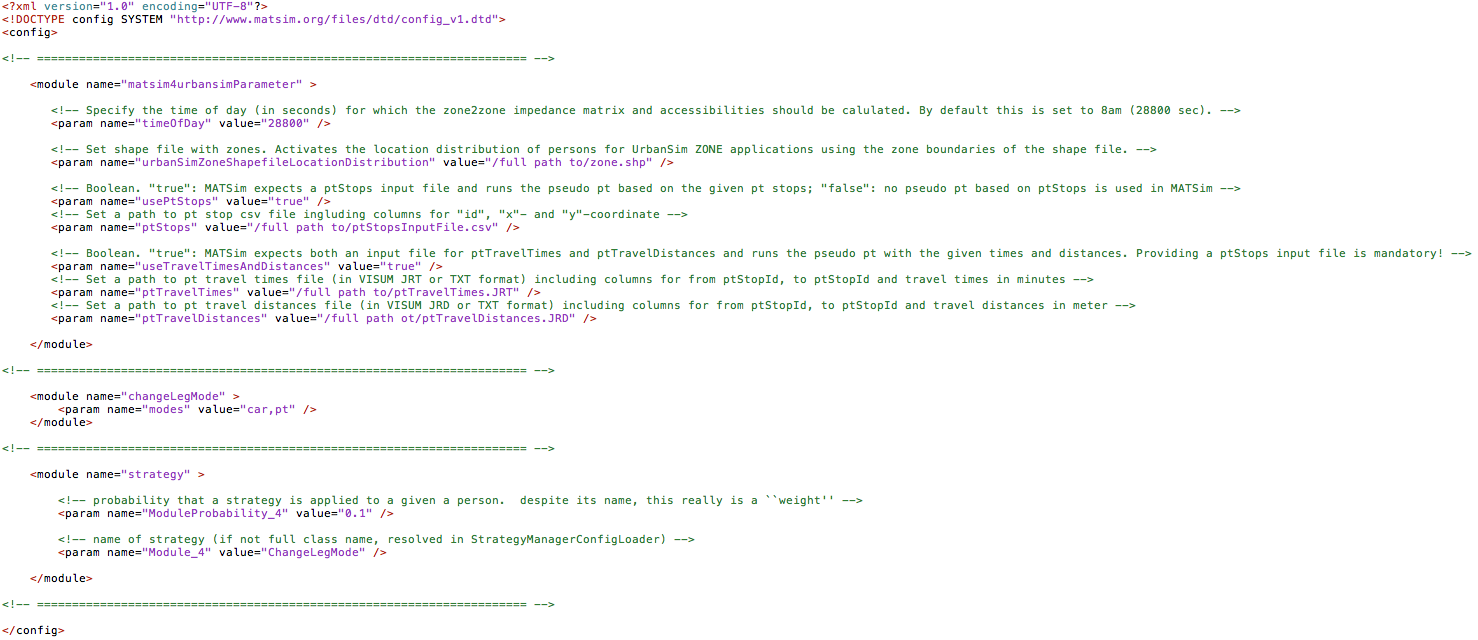
\includegraphics[width=\textwidth]{figures/matsim4urbansim/external_matsim_config_1.png}
\caption{Some addidional configuration settings for MATSim4UrbanSim  are only available/configurable via the standard MATSim configuration,  which are depicted in this illustration.}
\end{figure}

\begin{figure}[htp]
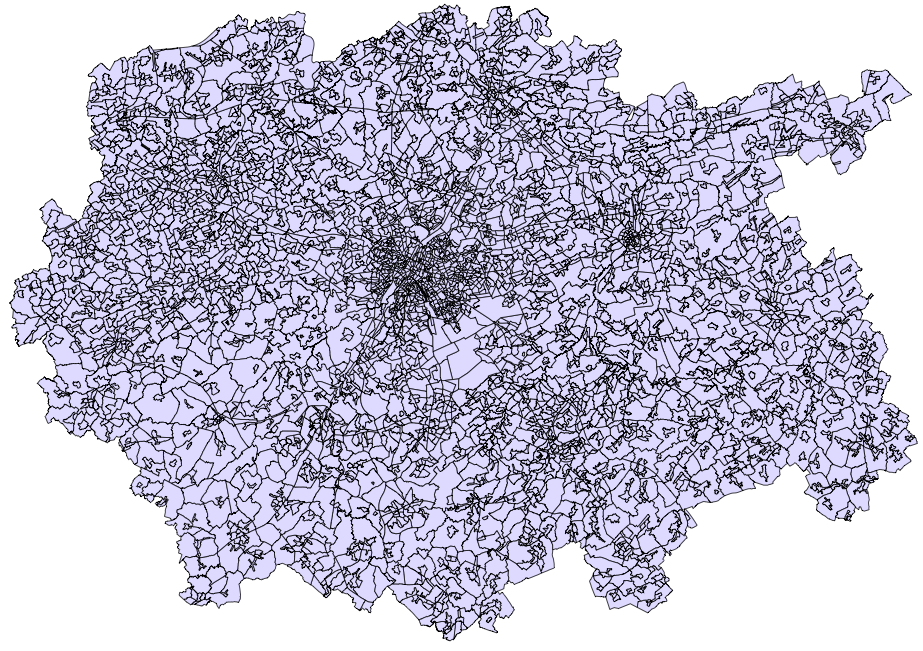
\includegraphics[width=\textwidth]{figures/matsim4urbansim/brussel_zone_shapefile.png}
\caption{A zone shape file at the example of the greater Brussels area.}
\end{figure}

\subsubsection{5 Create An Initial Plans File}

This section describes how to generate an initial plans file for warm  start. This example based on the Seattle parcel configuration, which  can be downloaded in section 3.
\begin{enumerate}
	\item Launch the OPUS GUI and open the sample Seattle parcel configuration.
	\item Switch to the Models tab and set the last iteration to 100" or higher
	\item Note: Leaving the population sample rate at 0.01 will generate a 1\% plans file
	\item Switch to the Scenarios tab and right-click on "Seattle\_baseline" and then on "Run this Scenario" to start the simulation
	\item When the simulation finished find the plans file at  "OPUS\_HOME/matsim4opus/output/ITERS/it.100/100.plans.xml.gz" and move it  to a convenient place, e.g. into  "OPUS\_HOME/data/seattle\_parcel/base\_year\_data/2000/matsim/plans"
	\item Finally enter the relative path to the plans-file, i.e.  data/seattle\_parcel/base\_year\_data/2000/matsim/plans/100.plans.xml.gz,  into the \textbf{input\_start\_plans\_file }field in the OPUS GUI  under "travel model conguration $>$ matsim\_config $>$ common" to start  MATSim in warm start mode next time.
\end{enumerate}

\subsubsection{6 Travel Model Visualization}

There are at least two options to visualize the traffic in MATSim see \href{http://matsim.org/node/741}{here}.

\subsubsection{7 Limitations}

The Java virtual machine (VM) can't allocate more than 1.5 GB on  32bit Windows systems, no matter how much RAM is available in your  computer. For this reason the travel model plug-in runs MATSim with 1.5  GB on Windows (32bit and 64bit) and with 4 GB on Mac and Linux systems  by default. This may cause longer computing times on Windows  computers.

%%\vfill\eject
%%\subsection{MATSim4UrbanSim (Frist Release)}

%%\subsubsection{The current user guide can be found \href{http://matsim.org/docs/extensions/matism4urbansim}{here} !!!}



%%\subsubsection{Guide on UrbanSim usage of the travel model plug-in}

%%The current travel model plug-in implementation is applicable for  PSRC (Puget Sound Region Council) parcel, Seattle parcel and Zurich  parcel scenario.

%%Note that some of the instructions may change since the travel model plug-in is still under development.

%%\subsubsection{1 Prerequisites}

%%You must have installed UrbanSim, before getting started with the  travel model plug-in. The following provides an entry point to install  UrbanSim and continues with installation instructions for additional  software packages required by the travel model plug-in.

%%\subparagraph{Hints for installing UrbanSim}

%%To install UrbanSim please follow the UrbanSim Downloads and Installation Instructions on \href{http://urbansim.org/Download/}{http://urbansim.org/Download/}.

%%When installing OPUS and UrbanSim manually (Windows users may require  an additional svn client, e. g. totoisesvn, which is available for free  at \href{http://tortoisesvn.tigris.org/}{http://tortoisesvn.tigris.org/})  please make sure to get the source code for the stable release or the  latest development version as described in Downloading Sample Data and  Source Code on: \href{http://urbansim.org/Download/DownloadingSampleDataAndSourceCode}{http://urbansim.org/Download/DownloadingSampleDataAndSourceCode}.

%%Windows users using the installer are getting the source code and data automatically.

%%Finally make sure that all UrbanSim environment variables, meaning  OPUS\_HOME, OPUS\_DATA\_PATH and PYTHONPATH, are set as described in the  installation instructions, see \href{http://urbansim.org/Download/SixtyFourBitMachines}{http://urbansim.org/Download/SixtyFourBitMachines} for Windows, \href{http://urbansim.org/Download/MacintoshInstallation}{http://urbansim.org/Download/MacintoshInstallation} for Mac or \href{http://urbansim.org/Download/LinuxInstallation}{http://urbansim.org/Download/LinuxInstallation} for Linux.

%%Note:  For using the travel model plug-in it is sufficient only to install the  required Python packages, i. e. numpy, scipy, lxml, sqlalchemy and  elixir.

%%\subparagraph{MATSim4UrbanSim prerequisites}

%%In addition to the UrbanSim installation the MATSim travel model plug-in requires the following software installed:
%%\begin{itemize}
%%	\item Java JDK 1.6 or newer: Download and install the newest version  of the Java SE Development Kit (JDK) for your operating system from \href{http://www.oracle.com/technetwork/java/javase/downloads/index.html}{http://www.oracle.com/technetwork/java/javase/downloads/index.html}. Make sure adding Java's /bin directory to the PATH environment variable. Click\href{http://java.com/en/download/testjava.jsp}{here}to test ifjavaisalready installed on your computer.
%%	\item Python XML Schema Bindings (PyXB): Download the PyXB distribution file from \href{http://sourceforge.net/projects/pyxb/}{http://sourceforge.net/projects/pyxb/} and extract it to a convenient place. Windows users may use Win-Rar to extract tar or gz files, which is available for free at \href{http://www.win-rar.com/}{www.win-rar.com}.
%%\\
%%\\   Open a command prompt (Windows) or a terminal (Mac, Linux). To install  PyXB (this may requires administrator or root privileges) go into  the extracted directory and type
%%\\


%%\texttt{python setup.py install}
%%\end{itemize}

%%\subsubsection{2 MATSim4UrbanSim installation}

%%This section describes how to install MATSim4UrbanSim.

%%\subparagraph{Automatic installation}

%%Make sure to have the Python lib directory included to the  PYTHONPATH. This is the directory that contains the site-package  directory that is already included in the PYTHONPATH. The lib directory  should be something like


%%\texttt{C:$\backslash$Python2.6$\backslash$Lib$\backslash$ }for Windows,


%%\texttt{/Library/Frameworks/Python.framework/Versions/2.6/lib/} for Mac or


%%\texttt{/usr/lib/python2.6/} for Linux (Ubuntu).

%%To install MATSim4UrbanSim open command prompt (Windows) or a  terminal (Mac, Linux) and navigate to opus\_matsim/configs in the opus  source directory. Than type


%%\texttt{python install\_matsim4urbansim.py}

%%This creates the subdirectories matsim4opus/jar, loads required  MATSim executables and libraries and configures them. After the  installation the file/directory structure should look something like  Figure 1.

%%To test whether the MATSim4UrbanSim installation was successful follow the instructions described in Section 2.3.

%%Note: The installer will replace jar-files and libraries from a previous MATSim4UrbanSim installation.

%%\subparagraph{Manual installation}

%%In case that the automatic installation does not work follow these instructions:
%%\begin{itemize}
%%	\item Create the following directory structure in OPUS\_HOME: OPUS\_HOME/matsim4opus/jar
%%	\item Download the following files from \href{http://www.matsim.org/files/builds/}{http://www.matsim.org/files/builds/} into the jar directory:   
%%\begin{itemize}
%%	\item MATSim\_rXXXXX.jar (where XXXXX refers the current revision)
%%	\item MATSim\_libs.zip
%%	\item matsim4urbansim-X.X.X-SNAPSHOT-rXXXXX.zip (where XXXXX refers the current revision)
%%\end{itemize}
%%	\item Rename MATSim\_rXXXXX.jar into "matsim.jar".
%%	\item Extract the zip files MATSim\_libs.zip and matsim4urbansim-X.X.X-SNAPSHOT-rXXXXX.zip. After that the zip files can be removed.
%%	\item Rename the directory matsim4urbansim-X.X.X-SNAPSHOT-rXXXXX into  "contrib". Than navigate into contrib and rename the jar-file  matsim4urbansim-X.X.X-SNAPSHOT.jar into "matsim4urbansim.jar".
%%\end{itemize}

%%Be careful when renaming files or directories (i. e. make sure  that everything is written in lower case and check for spelling errors).  After the installation the file/directory structure in the matsim4opus  directory should look something like Figure 1. To test whether the  MATSim4UrbanSim installation was successful follow the instructions  described in Section 2.3.

%%\subparagraph{Test your MATSim4UrbanSim installation}

%%To test your installation open a command prompt (Windows) or a  terminal (Mac, Linux) and navigate to opus\_matsim/tests in the opus  source directory (PYTHONPATH). Then type


%%\texttt{python travel\_model\_test.py}

%%This starts a test scenario. If the test completes without errors, your travel model plug-in should be working.


%%%\includegraphics{User%27s%20Guide_files/structure.png}Figure 1: After the installation the matsim4opus directory should contain the depicted files and subdirectories.

%%\subsubsection{3 Using MATSim for UrbanSim}

%%This section aims to explain the MATSim travel model plug-in at the example of the Seattle\_parcel scenario.\textbf{ In order to run Seattle parcel with MATSim the following steps are necessary:} Download the\href{https://svn.vsp.tu-berlin.de/repos/public-svn/matsim/examples/countries/us/seattle/matsim.zip}{ matsim\_seattle.zip}  and unzip the file into your OPUS\_DATA/seattle\_parcel/base\_year/2000/  directory. After that your seattle\_parcel base year cache should look  like Figure 2. The zip-file contains a road network and a plans-file,  used by MATSim. Thesestepsalso apply for the PSRC scenario using\href{http://matsim.org/uploads/matsim_psrc.zip}{matsim\_psrc.zip} file.


%%%\includegraphics{User%27s%20Guide_files/seattle_parcel_base_year_dir.png}Figure  2: Put the unzipped "matsim" directory, including a road network and a  plans-file, into your seattle\_parcel base year cache in order to run  MATSim as a travel model for the Seattle\_parcel scenario.

%%In a recent effort the MATSim configuration is embedded into  UrbanSim. This enables the MATSim (travel model) plug-in in UrbanSim and  provides all necessary or basic options to run MATSim via the OPUS GUI.  To enable the MATSim plug-in requires the travel model configuration  section in the UrbanSim configuration as depicted in Figure 3.

%%Sample configurations, including the travel model configuration  section, can be found for the Seattle\_parcel (seattle\_parcel.xml) and  PSRC\_parcel (psrc\_parcel.xml) scenario in the opus source directory at  opus\_matsim/configs.

%%Windowsuserswill need to replaceslashesinpathsbybackslashes, e.g. replace "data/seattle\_parcel/base\_year\_data/2000/matsim/network/psrc.xml.gz" by "data$\backslash$seattle\_parcel$\backslash$base\_year\_data$\backslash$2000$\backslash$matsim$\backslash$network$\backslash$psrc.xml.gz".


%%%\includegraphics{User%27s%20Guide_files/configuration.png}Figure  3: Adding the travel\_model\_configuration section into an UrbanSim  configuration enables the MATSim plug-in and configuration options  within OPUS GUI.

%%\subparagraph{Travel Model configuration options}

%%This sections explains step by step the MATSim configuration options provided by the travel model plug-in.

%%Launch the OPUS GUI and open the Seattle\_parcel sample configuration  located at opus\_matsim/config/seattle\_parcel.xml in opus source  directory. Switch to the Models tab to get to the travel model  configuration section as shown in Figure 4. The following options are  available:
%%\begin{itemize}
%%	\item \textbf{Models}: The models section contains three models integrating MATSim into UrbanSim:   
%%\begin{itemize}
%%	\item Get\_cache\_data\_into\_matsim generates input data for MATSim and stores it a specified location.
%%	\item Run\_travel\_model executes MATSim.
%%	\item Get\_matsim\_data\_into\_cache imports the results of the traffic simulation for the next UrbanSim iteration.
%%	\item By default all models are enabled. Only disable models if you know what you are doing.
%%\end{itemize}
%%\end{itemize}
%%\begin{itemize}
%%	\item \textbf{MATSim4UrbanSim}: This section contains options concerning the interaction of both simulation models MATSim and UrbanSim.   
%%\begin{itemize}
%%	\item The sampling\_rate determines the percentage of considered  travellers for a MATSim run. 0.01 means that only one percent of  travelers are considered for the traffic simulation. This option allows  to speed up computations on the MATSim side, e. g. during testing a  scenario.
%%	\item Note that low sampling rates cause some peculiarities in terms of  realism. In this situation results are useful for sketch planning only,  not for quantitative analysis. Higher sampling rates need more ram and  hard drive space.
%%\end{itemize}
%%	\item \textbf{MATSim Config}: The common subsection provides some basic configuration option for MATSim.   
%%\begin{itemize}
%%	\item The matsim\_network\_file points, as the name implies, to a road  network in MATSim format. This expects a relative path to the network  file located in the OPUS\_HOME directory.
%%	\item Determine the number of MATSim iterations with the item last iteration. In MATSim iterations start at zero.
%%\end{itemize}
%%\end{itemize}
%%\begin{itemize}
%%	\item \textbf{Years\_To\_Run}: This defines the years in which the travel model should run.
%%\\
%%\\   Adding additional years requires to edit the configuration file  directly, e. g. with a xml editor, within the year\_to\_run section in the  travel\_model\_configuration. Make sure that each year you are adding is  surrounded by the run\_description tags like this:
%%\end{itemize}


%%\texttt{ $<$run\_description type="directory"$>$}


%%\texttt{  $<$year type="integer"$>$2002$<$/year$>$}


%%\texttt{ $<$/run\_description$>$}

%%All configuration options can be easily edited in the OPUS GUI by clicking on the value or check box on the right hand side.


%%%\includegraphics{User%27s%20Guide_files/opus_gui.png}Figure 4: Configuring MATSim via the travel model configuration section in OPUS GUI.

%%\subsubsection{4 Travel Model Visualization}

%%There are at least two options to visualize the traffic in MATSim:
%%\begin{enumerate}
%%	\item \href{http://matsim.org/docs/extensions/otfvis}{OTFVis}
%%	\item \href{http://senozon.com/products/via}{Senozon via}
%%\end{enumerate}

%%\subsubsection{5 Limitations}

%%\subsubsection{The Java virtual machine (VM) can't allocate more  than 1.5 GB on Windows systems, no matter how much RAM is available in  your computer. For this reason the travel model plug-in runs MATSim with  1.5 GB on Windows and with 2 GB on Mac and Linux systems by default.  This may cause longer computing times on Windows computers.}

%%\vfill\eject
\subsection{The MATSim network for the Brussels application}

\subsubsection{Note:}

The current MATSim network for the Brussels case study can be downloaded \href{https://svn.vsp.tu-berlin.de/repos/public-svn/matsim/examples/countries/be/brussels/network/belgium_incl_borderArea_hierarchylayer4_clean_simple.xml.gz}{here}! In the following it is described step by step how this network is created by using Open Street Map (OSM).

\subsubsection{Step 1:}

The network for the Brussels case study is composed of separate OSM  networks for Belgium and its bordering regions in the Netherlands,  Germany, Luxembourg and France. The following OSM files are used, which  are available at \href{http://download.geofabrik.de/osm/europe/}{http://download.geofabrik.de/osm/europe/}:
\begin{itemize}
	\item  alsace.osm.bz2
	\item  belgium.osm.bz2
	\item  champagne-ardenne.osm.bz2
	\item  lorraine.osm.bz2
	\item  luxembourg.osm.bz2
	\item  netherlands.osm.bz2
	\item  nord-pas-de-calais.osm.bz2
	\item  nordrhein-westfalen.osm.bz2
	\item  picardie.osm.bz2
	\item  rheinland-pfalz.osm.bz2
	\item  saarland.osm.bz2
\end{itemize}

\subsubsection{Step 2:}

These OSM files are now merged to a coherent OSM network in a two  step process using the java command line application Osmosis. A deteiled  manual for Osmosis can be found at \href{http://wiki.openstreetmap.org/wiki/Osmosis}{http://wiki.openstreetmap.org/wiki/Osmosis}.
\begin{itemize}
	\item In the first step each OSM network is treated separately on the command line as follows:
\end{itemize}
\begin{verbatim}
osmosis --rx xxx.osm.bz2 --lp interval=60 --bb top=51.671 left=2.177 \
    bottom=49.402 right=6.764 completeWays=yes --tf accept-ways \
    highway= motorway,motorway_link,trunk,trunk_link,primary,primary_link,secondary,\
    tertiary,minor,unclassified,residential,living_street --tf reject-relations \
    --used-node --wx xxx_filtered.osm.bz2
\end{verbatim}

This modifies each network file as follows:
\begin{itemize}
	\item The network links and nodes that are  located in the area of interest are extracted. This area, defined by a  rectangle containing Belgium and its bordering regions.
	\item Links and nodes that do not correspond  to one of the following road types in OSM, for instance links and nodes  belonging railways, are removed: motorway, trunk, primary, secondary,  tertiary, minor, unclassified, residential and living street.
\end{itemize}
\begin{itemize}
	\item In the second step, the modified networks are merged on the command line as follows:
\end{itemize}
\begin{verbatim}
osmosis --rx xxx_filtered.osm.bz2 --lp interval=30 --m --wx belgium_incl_borderArea.osm
\end{verbatim}

At this point we have one merged OSM network "belgium\_incl\_borderArea.osm" for our area of interest.

\subsubsection{Step 3:}

The merged OSM network is converted into MATSim format. To be  consistent with the UrbanSim coordinates in the Brussels case study the  MATSim default network coordinates are transformed using the \emph{Belge Lambert 72}  projection. One hierarchy level is used to avoid side effects of having  different network densities within and around the study area. The used  hierachy level includes, in OSM terms, links and nodes of secondary  roads or greater.

Finally the MATSim network is “cleaned” and “simplified”. Cleaning  means, that only links that can be reached by other links are kept in  the network. Simplifying means, that a set of links that belong to a  road are merged into one single link. The resulting network is depicted  below, where the study area is highlighted in blue.

The Java code for the conversion is given in here:
\begin{lstlisting}{language=Java}
Scenario sc = ScenarioUtils.createScenario(ConfigUtils.createConfig());
// creating an empty matsim network
Network network = sc.getNetwork();
// using the Belge Lambert 72 projection for the matsim network
CoordinateTransformation ct = TransformationFactory
        .getCoordinateTransformation(TransformationFactory.WGS84, "EPSG:31300");
OsmNetworkReader osmReader = new OsmNetworkReader(network, ct);

osmReader.setKeepPaths(false);
osmReader.setScaleMaxSpeed(true);

// this layer covers the whole area, Belgium and bordering areas
// including OSM secondary roads or greater
osmReader.setHierarchyLayer(51.671, 2.177, 49.402, 6.764, 4);

// converting the merged OSM network into matsim format
osmReader.parse(INFILE);
new NetworkWriter(network).write(OUTFILE);
// writing out a cleaned matsim network and loading it
// into the scenario
new NetworkCleaner().run(OUTFILE, OUTFILE.split(".xml")[0] + "_clean.xml.gz");
Scenario scenario = (ScenarioImpl) ScenarioUtils
        .createScenario(ConfigUtils.createConfig());
new MatsimNetworkReader(scenario).readFile(OUTFILE.split(".xml")[0] + "_clean.xml.gz");
network = (NetworkImpl) scenario.getNetwork();

// simplifying the cleaned network
NetworkSimplifier simplifier = new NetworkSimplifier();
Set<Integer> nodeTypess2merge = new HashSet<Integer>();
nodeTypess2merge.add(new Integer(4));
nodeTypess2merge.add(new Integer(5));
simplifier.setNodesToMerge(nodeTypess2merge);
simplifier.run(network);
new NetworkWriter(network).write(OUTFILE.split(".xml")[0] + "_clean_simple.xml.gz");
\end{lstlisting}




%\includegraphics{User%27s%20Guide_files/belgium_incl_borderArea_hierarchylayer4_clean_simple.png}


\vfill\eject
\NextFile{OTFVis.html}
\section{OTFVis}

OTFVis  is a visualizer for MATSim. It can be used to replay snapshots of  simulations, or run a simulation and interact with it. The visualizer  makes use of hardware acceleration (OpenGL) and is thus also suitable  for visualizing large scenarios. If you have problems running OTFVis,  make sure to \href{http://www.matsim.org/docs/extensions/otfvis/opengl}{check your Graphics Card is able to support OTFVis}.

\subsection{Download / Requirements}

To use OTFVis, you need MATSim as well as the OTFVis extension. The  OTFVis extension is not yet available as an official release, so the  following documentation will use a nightly build of it.
\begin{itemize}
	\item Download a current nightly build of MATSim, the MATSim libraries and OTFVis from our \href{http://www.matsim.org/files/builds}{nightly build download page}.
	\item Unzip the MATSim libs
	\item Unzip the OTFVis Extension
\end{itemize}

You should now have: the MATSim jar, the libs directory, and the otfvis directory next to each other.

\subsection{Starting the Visualizer}

The main class for the visualizer is 
\texttt{org.matsim.contrib.otfvis.OTFVis}. The different ways to start OTFVis will be described in more details below.

The visualizer may require a lot of memory, it is thus advised to start it with the corresponding Java options, e.g. with 500MB:
\begin{verbatim}
java -Xmx500m-cp MATSim.jar:otfvis/otfvis.jarorg.matsim.contrib.otfvis.OTFVis arguments
\end{verbatim}

If you're on Windows, use 
\texttt{;} instead of 
\texttt{:} to  separate the jar files from each other. Also, depending on the version  you downloaded, you might have to adapt the file and directory names a  little bit.  

\subsection{Creating snapshots (mvi-files) from Events}

Use the following arguments:
\begin{verbatim}
-convert event-file network-file mvi-file [snapshot-period]
\end{verbatim}

to record a snapshot of all vehicles' positions every snapshot-period  seconds, based on the events and network given in the corresponding  files.

Example call:
\begin{verbatim}
java -cp MATSim.jar:otfvis/otfvis.jarorg.matsim.contrib.otfvis.OTFVis -convert output/50.events.txt.gz input/network.xml.gz output/50.visualization.mvi 300


\end{verbatim}

This will create a snapshot of every 5th minute and store it in the file 
\texttt{output/50.visualization.mvi}.

\subsection{Displaying MATSim Visualization Snapshots (mvi-files)}

Just pass the file as first argument. Example call:
\begin{verbatim}
java -cp MATSim.jar:otfvis/otfvis.jarorg.matsim.contrib.otfvis.OTFVis output/0.visualization.mvi
\end{verbatim}

\subsection{Displaying TRANSIMS Vehicle files}

For reasons of backward compatibility, OTFVis can display vehicles  files traditionally generated by TRANSIMS. As the vehicle file does not  include any network information, the network must be passed as well.  Example call:
\begin{verbatim}
java -cp MATSim.jar:otfvis/otfvis.jarorg.matsim.contrib.otfvis.OTFVis output/0.T.veh input/network.xml.gz
\end{verbatim}

\subsection{Displaying MATSim Network files}

OTFVis can display just a network. This is useful when building a  scenario, and a network converted from other data must be inspected.  Example call:
\begin{verbatim}
java -cp MATSim.jar:otfvis/otfvis.jarorg.matsim.contrib.otfvis.OTFVis input/network.xml.gz
\end{verbatim}

(Note: Currently only available in Nightly Builds since revision r5821)

\subsection{Start Interactive Simulation}

OTFVis can directly start a simulation and visualize it in real time.  As in that case, all data (esp. the population) is loaded into memory,  interactive queries about agents and link states can be issued from the  visualizer. To start OTFVis in this interactive, live mode, just pass it  the config-file you would otherwise pass to the Controler:
\begin{verbatim}
java -cp MATSim.jar:otfvis/otfvis.jar org.matsim.contrib.otfvis.OTFVis input/config.xml
\end{verbatim}

Please note that this will require even more resources (memory, cpu-speed) than only running the simulation with the Controler.

\subsection{Running OTFVis from within a windows systems}

As shown by the \href{http://www.matsim.org/downloads/nightly}{Nightly Builds}  tutorial OTFVis and other classes can be run by using the command line  or a shell script respectively. As the Unix based way is already  described by the tutorial, this is about the windows user.

The windows command line call looks similiar to the Unix based one. Finally, you should end with something like that
\begin{verbatim}
java -Xmx1500m -cp MATSim.jar:otfvis/otfvis.jarorg.matsim.contrib.otfvis.OTFVis %*
\end{verbatim}

which can be saved as a *.bat file, e.g. otfvis.bat. Please note that  the example is based on the assumption that otfvis.bat is saved in the  same folder as the matsim.jar and the libs folder. The placeholder \%*  will be substitued by the parameters you've specified when calling  otfvis.bat from the command line, e.g.
\begin{verbatim}
otfvis.bat -convert event-file network-file mvi-file
\end{verbatim}

To call the OTFVis from any folder, put the otfvis.bat into your PATH environment.

If your are more familiar with the point and click behaviour of win  systems, you can create a shortcut pointing to your otfvis.bat.
\begin{enumerate}

	\item By putting it on your desktop, you can drop any file on it, to call OTFVis with the file dropped, e.g. a network.

	\item 
Move  the shortcut to your SendTo folder and rename it to something like  OTFVis.lnk. Depending on the system you use, the SendTo folder should be  located in your home directory. Now you can start the OTFVis by  rightclicking at any file within your system, e.g. rightclick a  mvi-file, from the context menu select SendTo -$>$ OTFVis.

%\includegraphics{User%27s%20Guide_files/moz-screenshot.jpg}

\end{enumerate}



\vfill\eject
\subsection{OpenGL Requirements}

For  the hardware acceleration to work, (i) the OpenGL graphic card driver  installed on your machine must be at least of version 2.0 and (ii)  native libraries are required, which must be correctly set up.

\subsubsection{Check and Update Graphic Card Driver}

Either you use check and update mechanims / software already  installed (e.g. NVIDIA software, ATI update manager, etc...) or download  and install \href{http://www.realtech-vr.com/glview}{OpenGL Extension Viewer}.  After starting this little tool, it show all necessary information  abour your graphic card including OpenGL version. Please be sure that at  least \textbf{OpenGL version 2.0} is installed. Otherwise try  to find approriate driver updates of your graphic card (the read circles  in the Figure below shows the important featrues / information).


%\includegraphics{User%27s%20Guide_files/openglextensionviewer_png_4b5038ca1c.html}


\vfill\eject
\NextFile{TransEnergySim.html}
\section{Transportation Energy Simulation Framework (transEnergySim)}

\subsection{[module is still under construction]}

In this MATSim contribution a framework to simulate a whole range  oftranportation related energy scenarios is implemented. The focus  is on electric and plug-in hybrid electric vehicles. This contributio  is being built and updated as part of the PhD ofRashid A. Waraich  (waraich at ivt.baug.ethz.ch). As this is an open source project, which  encourages contribution by others, there are also modules, which have  been contriubted by the following people: Dr. Matthias D. Galus, Gil  Georges ?, Marina ?, Zain?, Raffaela?, etc.?


The following modules should be available soon/ are planned:
\begin{itemize}
	\item Inductive charging along roads
	\item Charging at activity location
	\item Several charging schemes including smart charging ("smart grid")
	\item V2G
	\item General energy flow model
	\item buy/sell of electricity price over market
\end{itemize}

These features require several basic constructs, which willalso be documented soon here:
\begin{itemize}
	\item vehicle fleet definition model
	\item vehicle energy consumption model
	\item charging infrastructure definition model
	\item output modules
	\item more to come here...
\end{itemize}

If you want to contribute with a new module to the framework  (e.g. for charging, energy consumption, emissions, etc.), please contact  Rashid A. Waraich (waraich at ivt.baug.ethz.ch).

\subsection{Applications}

TODO: Describe ARTEMIS and THELMA project here with figures and references.



TODO: also add work of stella, zain, raffaela, marina, etc. here.

\subsection{Emissions}

Modules for green house gas and other emissions coming soon here.

\subsection{Hints and Pitfalls}

ParallelEventHandling

Many of the modules for keeping track of charging and energy  consumption are based on event handlers. In order to avoid  raceconditions and accessing the same data unsynchronized (e.g. vehicle  trying to charge before the energy consumption is updated), we advise to  use the EventHandlerGroup class (or inherit from it, if needed). Using  this class, you can clearly control, which thing happens first, e.g.  energy consumption updated first and trying to charge happening  afterwards (also important for road charging). For an example, see the  InductiveChargingController.

At the moment, the it does not seem to be a performance issue, to  group several modules together (forming effectivly one event handler).  But if there are concerns about this, a synchronized version could be  provided in future.

\subsection{Inductive Charging}

Charging along Roads

For Inductive charging along roads the InductiveStreetCharger Module  can be used, which is based on event handlers. An example controller,  which allows both stationary charging at activitiy locations and  charging at roads is calledInductiveChargingController. General  help regarding how to configure the controller, can be found in a test  of the controller and the documentation of the different modules, which  are used in that controller.

(TODO: add links to the code/test cases)



Stationary Inductive Charging

This is currently not distinguished separatly from stationary charging with a plug, although it might be in future.

\subsection{Stationary Charging}

For stationary charing, at the moment the following modules are available:

ChargingUponArrival: Vehicles with a state of charge (SOC) smaller  than the "usable battery size" start charging immediatly opon arrival at  a location. TODO: descibe, how to filter the location, where vehicle  can be charged.

\subsection{Vehicle Energy Consumption Models}

Each  vehicle in the vehicle has an Energy consumption model attached to it,  based on which vehicle energy consumption is logged for each street.  Furthermore for electric and plug-in hybrid electric vehicles (EV/PHEV),  this module also updates the state of charge (SOC) of the vehicles.

A couple of models are available for use, of which many have been  contributed by the respective authors of the models. If you want to  contribute a new model, please drop an email to  waraich@ivt.baug.ethz.ch.

Electric Vehicle



PHEV

Galus Model

TODO: also show shape of curve!



Conventional Vehicle

(no model available at the moment)

\subsection{Visualizations}

TODO: emissions map, charging acts, power load per link, etc.




%\appendix
%\chapter*{Appendices}
%\addcontentsline{toc}{chapter}{Appendices}
%\markboth{Appendices}{}%fix headers



%%%%%%%%%%%%%%%%%%%%%%%%%%%%%%%%%%%%%%%%%%%%
%%%%%%%%%%%%%%%%%%%%%%%%%%%%%%%%%%%%%%%%%%%%


\umbruch
%%%%%%%%%%%%%%%%%%%%%%%%%%%%%%%%%%%%%%%%%%%%
%%%%%%%%%%%%%%%%%%%%%%%%%%%%%%%%%%%%%%%%%%%%
%%%%%%%%%%%%%%%%%%%%%%%%%%%%%%%%%%%%%%%%%%%%
%%%%%%%%%%%%%%%%%%%%%%%%%%%%%%%%%%%%%%%%%%%%
\end{document}



% Local Variables:
% mode: latex
% mode: reftex
% mode: visual-line
% comment-padding: 1
% fill-column: 999
% End: 
